\documentclass[review]{elsarticle}

\usepackage{lineno,hyperref,amsmath,amsfonts,subcaption}
\modulolinenumbers[5]

\journal{Spatial Statistics}

%%%%%%%%%%%%%%%%%%%%%%%
%% Elsevier bibliography styles
%%%%%%%%%%%%%%%%%%%%%%%
%% To change the style, put a % in front of the second line of the current style and
%% remove the % from the second line of the style you would like to use.
%%%%%%%%%%%%%%%%%%%%%%%

%% Numbered
%\bibliographystyle{model1-num-names}

%% Numbered without titles
%\bibliographystyle{model1a-num-names}

%% Harvard
\bibliographystyle{model2-names.bst}\biboptions{authoryear}

%% Vancouver numbered
%\usepackage{numcompress}\bibliographystyle{model3-num-names}

%% Vancouver name/year
%\usepackage{numcompress}\bibliographystyle{model4-names}\biboptions{authoryear}

%% APA style
%\bibliographystyle{model5-names}\biboptions{authoryear}

%% AMA style
%\usepackage{numcompress}\bibliographystyle{model6-num-names}

%% `Elsevier LaTeX' style
%\bibliographystyle{elsarticle-num}
%%%%%%%%%%%%%%%%%%%%%%%

\begin{document}

\begin{frontmatter}

\title{Spatial log-Gaussian Cox process models and sampling paths: Toward optimal design}

%% Group authors per affiliation:
\author[msuaddr]{Kenneth Flagg\corref{mycorrespondingauthor}}
\cortext[mycorrespondingauthor]{Corresponding author}
\ead{kenneth.flagg@montana.edu}

\author[msuaddr]{John Borkowski}
\author[msuaddr]{Andrew Hoegh}

\address[msuaddr]{Department of Mathematical Sciences, Montana State University, Bozeman, MT 59717}

\begin{abstract}

The log-Gaussian Cox (LGCP) process model is becoming the go-to model for
spatial point pattern data as fast Bayesian computing methods are removing the
barriers to its use. In many applications, such as unexploded ordnance
remediation and species distribution studies, a sampling procedure is used in
which only events near a one-dimensional path are observed. Very little work
has been done regarding optimal design of these paths. We present a variety of
path designs and user simulations to compare them in terms of model-based
spatial prediction criteria. We also define a spatial coverage statistic for
path designs, the average distance-to-path. We show that, when total length is
limited, paths with regular spacing and direction changes provide small errors
and low posterior variance while being relatively robust against computational
artifacts. For longer paths, systematic line-transect designs perform well.

\end{abstract}

\begin{keyword}
spatial point process\sep log-Gaussian Cox process\sep optimal sampling\sep model-based design\sep spatial sampling design
%\MSC[2010] 00-01\sep  99-00
\end{keyword}

\end{frontmatter}

\linenumbers

% Can name paragraphs with \paragraph{Title}


\section{Introduction}
% State the objectives of the work and provide an adequate background, avoiding a detailed literature survey or a summary of the results.

Spatial point process models have generally been infeasible because of their
computational demands, but recent advances in Bayesian computing have made the
Log-Gaussian Cox process (LGCP) an attainable model in
practice~\citep{rueetal,lindgrenetal,illianetal,simpsonetal}. These advances
make it possible to fit LGCP models easily and quickly, without time-consuming
Monte Carlo methods.

In some spatial point process applications, the entire point pattern is not
fully observed due to variable sampling effort. This is referred to as a
partial or degraded point pattern~\citep{chakrabortyetal}. It is relatively
simple to accommodate variable sampling effort in these models using modern
Bayesian computing tools~\citep{yuanetal}. However, the literature on optimal
sampling for spatial point process models is in its
infancy~\citep{liuvanhatalo}.

Point pattern data are routinely collected in species distribution studies and
ordnance response projects. The data consist of the locations of events in some
spatial region. In many cases it is too costly to observe the entire study
region, so a sampling procedure is employed. These applications may use quadrat
sampling or line-transect sampling, with transect sampling being more common.
Software is now available to fit spatial point process models to data acquired
via distance sampling and simultaneously estimate the detection
function~\citep{dspat,baser}. Various spatial mapping procedures have been used
to map where events occur in space. However, these have traditionally involved
aggregating the data to grid cell counts or computing moving averages.
Aggregation has the downside of introducing arbitrary structure into the data
by the choice of grid scheme or averaging window, and requires unnecessary
computation effort~\citep{simpsonetal}.
% Recent example of aggregation: https://link-springer-com.proxybz.lib.montana.edu/content/pdf/10.1007/s13253-020-00386-3.pdf

In ecological settings, sampling plans are often designed around the goal of
estimating total abundance. Ordnance response surveys are typically designed
to provide enough data to detect (but not necessarily map) intensity
hotspots~\citep{em200-1-15,flaggetal}. However, %to our knowledge,
there has been very little work done in deciding \emph{where} to collect data
when the goal is to map the intensity using a spatial point process model.
While some ideas about the characteristics of a good point design apply to
paths, creating an optimal path design is not as simple as connecting the
points of a point design with line segments. There are many ways to connect
points into a path, so optimal design criteria must apply to the whole path and
not only to the waypoints.

In this paper, we develop a space-filling criterion for path designs, present
a variety of designs, and assess their utility for spatial prediction using
LGCP model fitting in terms of robustness to computational issues and
model-based criteria.


\subsection{Log-Gaussian Cox process}

The log-Gaussian Cox process (LGCP) is an inhomogeneous Poisson process where
the logarithm of the intensity function is a Gaussian process (GP;
\citealt{moelleretal}). The LGCP model provides a flexible model for mapping event
intensity over space using few parameters. Efficient Bayesian computation tools
are available using INLA to approximate the posterior marginal distributions
\citep{rueetal}, a finite element approach to represent the GP
\citep{lindgrenetal}, and pseudodata to approximate the point process
likelihood \citep{simpsonetal}.
% Add some example applications.


\subsection{Spatial design}

Most classical sampling and design work has been done for points, or for small
quadrats approximated as points, rather than for paths. In two-dimensional
geostatistical model-based design, regular spacing is optimal for spatial
prediction but randomness and a variety of interpoint distances are best for
parameter estimation~\citep{diggle}. Inhibitory plus close pairs designs are a
good compromise when estimation and prediction are both
important~\citep{chipetaetal2017}.

Design-based approaches exist to spread points through high-dimensional design
spaces~\citep{borkowskipiepel}, and Latin hypercube sampling has space-filling
characteristics~\citep{mckayetal,husslageetal}. Minimax and maximin distance
are popular criteria for ensuring deign points represent the entirety of a
large (or high-dimensional) design space~\citep{johnson}. These criteria
are calculated from the distances between design points and arbitrary
points in the design space, explicitly ensuring coverage by minimizing the
maximum distance between the design space and the design (minimax) or
maximizing the minimum distance between pairs of design points (maximin).


\subsection{Space-filling curves}

A relevant area of mathematical research is in deterministic space-filling
curves. These have been used in the design of dense or stretchable
circuits~\citep{ogorzalek,mazhang} and high-dimensional data visualization
in bioinformatics~\citep{hilbertvis}. They are appealing as path designs
because, given enough length, the path will visit every part of the study site.

Example space-filling curves include the Hilbert curve, which is simple to
construct, and the Peano curve, which is very flexible for filling irregular
shapes \citep{fanetal}. Space-filling curves are one-dimensional paths
constructed iteratively; as the number of iterations goes to infinity, the
limiting path has nonzero area and actually fills the space~\citep{sagan}. For
applications we stop after a finite number of iterations.


\subsection{Paths as sampling designs}

The small body of literature on spatial sampling design for point pattern
data has focused on line transects. \citet{pollard} began with line transects
and adaptively added zigzags in a species abundance survey. The Visual Sample
Plan software, commonly used for design and data analysis in ordnance
remediation projects, includes features to create systematic transect plans
and augment plans with additional transects in regions lacking spatial
coverage~\citep{vspguide}. It helps the user choose the transect spacing to
maximize the probability of detecting the presence of a hotspot of specified
size and intensity. However, it does not employ criteria to optimize spatial
prediction. \citet{liuvanhatalo} provided one of the first explicit discussions
of design in the context of spatial LGCP models. The study used narrow quadrats
(swaths along line-transects) as the sampling units. The transects were short
relative to the size of the study region and not connected into a path, so they
were treated as disconnected points for the purposes of design construction.


\subsection{Goals of this paper}

We have two broad goals for this paper. First, we will illuminate the current
state of practical computing for LGCP models fit to degraded point patterns
observed via survey sampling. Second, we open discussion of path design for
LGCP models by identifying design schemes that are promising for field use.

We accomplish these goals via a simulation study, using many designs each
applied to the same simulated datasets. The simulated data collection procedure
is based upon geomagnetic surveys for unexploded ordnance, where metal
detectors traverse a path and detect events under their footprint, i.e. within
a fixed, and assumed known, width centered on the path. The paths are long
enough that they cannot be approximated by discrete design points.


\section{Materials and methods}
% Provide sufficient details to allow the work to be reproduced by an independent researcher. Methods that are already published should be summarized, and indicated by a reference. If quoting directly from a previously published method, use quotation marks and also cite the source. Any modifications to existing methods should also be described.

%Kenny's heuristics of a good path design:
%\begin{itemize}
%\item Should start with a sparse design with regular spacing, then refine with
%infill
%\begin{itemize}
%\item Provides good spatial coverage even if aborted early
%\item Imagine downloading a high-resolution intensity jpeg over 56k
%\end{itemize}
%\item Path should avoid sharp turns but is allowed to cross itself
%\item One option is to generate two segments at a time, first a short-to-medium
%length segment to get to the start of the next transect, then a  medium-to-long
%segment for the transect
%\item Could have new segment length be negatively correlated with the previous
%segment length
%\end{itemize}

With an eye toward practical considerations of data collection, we present
criteria to compare sampling strategies that impact LGCP model fitting and
posterior inferences. We compare plans with (approximately) fixed path lengths,
most of which avoid sharp turns. Data collection equipment (e.g. vehicle-towed
metal detectors) may have limited maneuverability, requiring minimizing the
number or angle of turns. This section describes the designs in detail, then
introduces notation and design criteria, and finally summarizes the
computational model-fitting approach.


\subsection{Sampling design schemes}
\label{methodschemes}

In this section, we present three variations of parallel line transect designs
and three schemes that produce more complex designs. To clarify terminology, a
\emph{path} or \emph{design} is a realized set of one or more connected
components with length but not area. The paths considered in this work are
constructed as sequences of line segments. A \emph{design scheme}, or simply
\emph{scheme}, is a procedure for generating designs with some shared
characteristics. Figure~\ref{plancomparison} illustrates a selection of designs
from these schemes.


\subsubsection{Parallel line transects}

Parallel straight-line transects are common in ordnance response studies and in
ecological studies using distance sampling. Systematic designs are popular
because they provide good spatial coverage in the sense that any point in the
study site has an a priori known maximum distance from the path. For point
designs, systematic designs are preferred for prediction, simple random samples
are good for estimation, and inhibitory with close pairs designs are becoming a
popular compromise~\citep{chipetaetal2017}. We adapt all three of these to the
parallel line transect setting. We use line transects running north-south, with
three methods of choosing the horizontal coordinate: simple random sample
(SRS), systematic with a random starting point and fixed spacing, and
inhibitory plus close pairs. Figure~\ref{plancomparison} (left column) shows an
example of each scheme with 25 transects. Additional examples appear in
Appendix~\ref{moreplots}.

%We should note that we will be using an isotropic covariance function in
%the model. If an anisotropic model is used, parallel transects may need to be
%augmented with perpendicular transects so that the observed data provide the
%full range of pairwise distances in other directions.

\begin{figure}

\begin{subfigure}{2.5in}
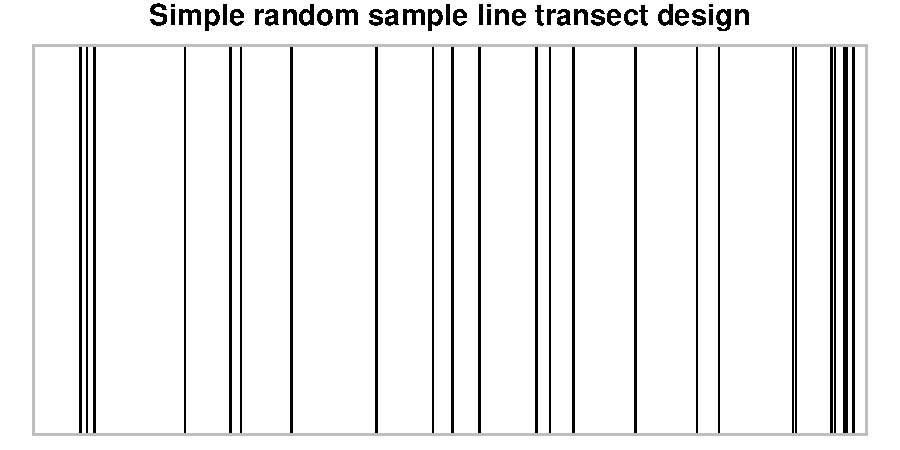
\includegraphics[width=2.5in]{../graphics/SRS000176.pdf}
\caption{SRS of 25 parallel transects}
\label{srs000176}
\end{subfigure}
\begin{subfigure}{2.5in}
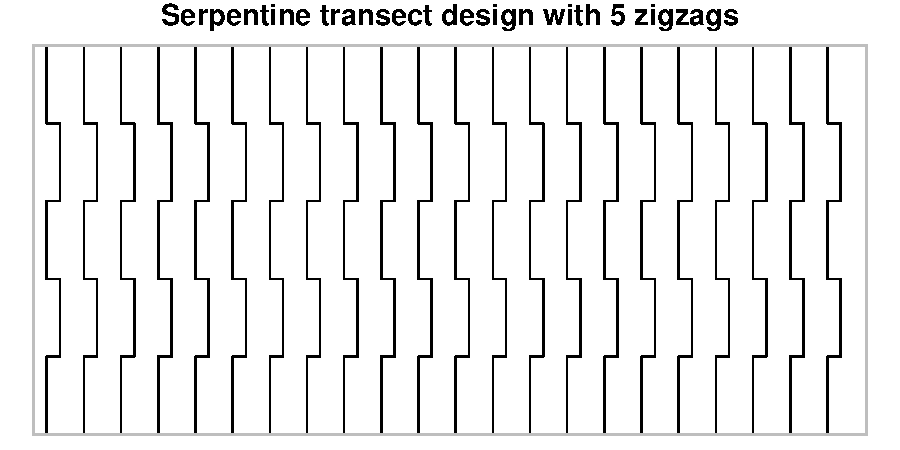
\includegraphics[width=2.5in]{../graphics/Serp000124.pdf}
\caption{Serpentine design with fewer corners}
\label{serp000124}
\end{subfigure}

\begin{subfigure}{2.5in}
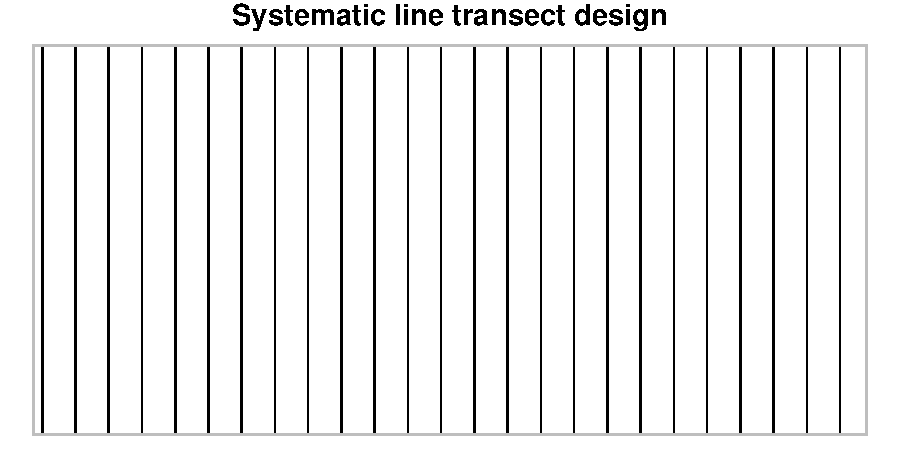
\includegraphics[width=2.5in]{../graphics/Sys000141.pdf}
\caption{Systematic design of 25 parallel transects}
\label{sys000141}
\end{subfigure}
\begin{subfigure}{2.5in}
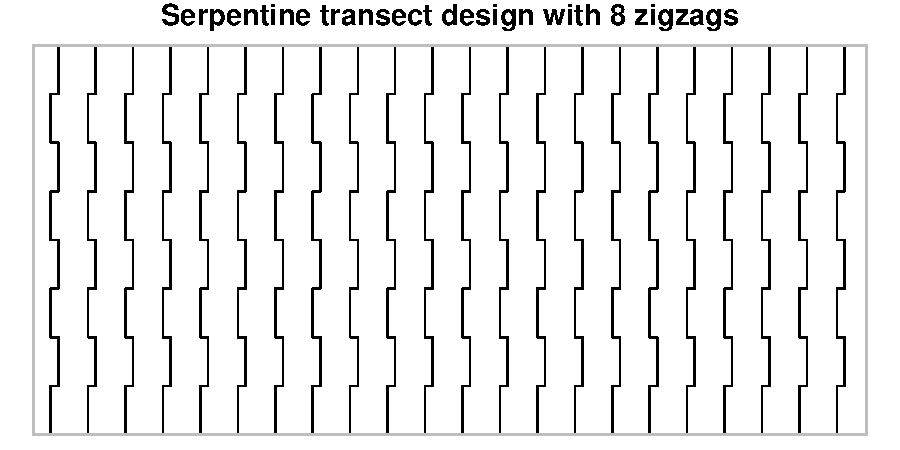
\includegraphics[width=2.5in]{../graphics/Serp000539.pdf}
\caption{Serpentine design with more corners}
\label{serp000539}
\end{subfigure}

\begin{subfigure}{2.5in}
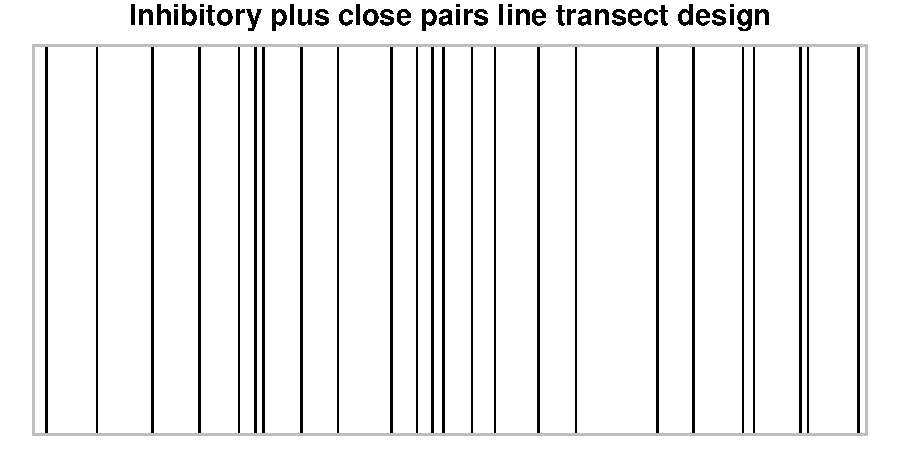
\includegraphics[width=2.5in]{../graphics/Inhib000171.pdf}
\caption{Inhibitory/pairs design with 25 transects}
\label{inhib000171}
\end{subfigure}
\begin{subfigure}{2.5in}
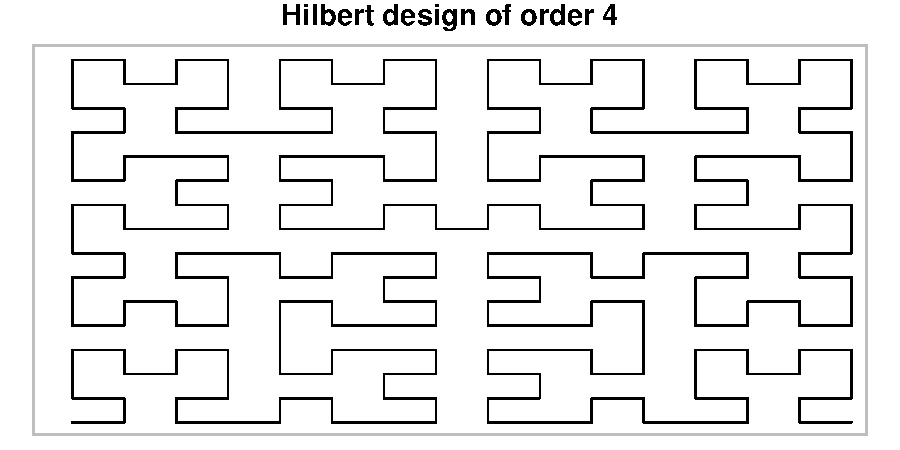
\includegraphics[width=2.5in]{../graphics/Hilbert000180.pdf}
\caption{Space-filling Hilbert design, less refined}
\label{hilbert000180}
\end{subfigure}

\begin{subfigure}{2.5in}
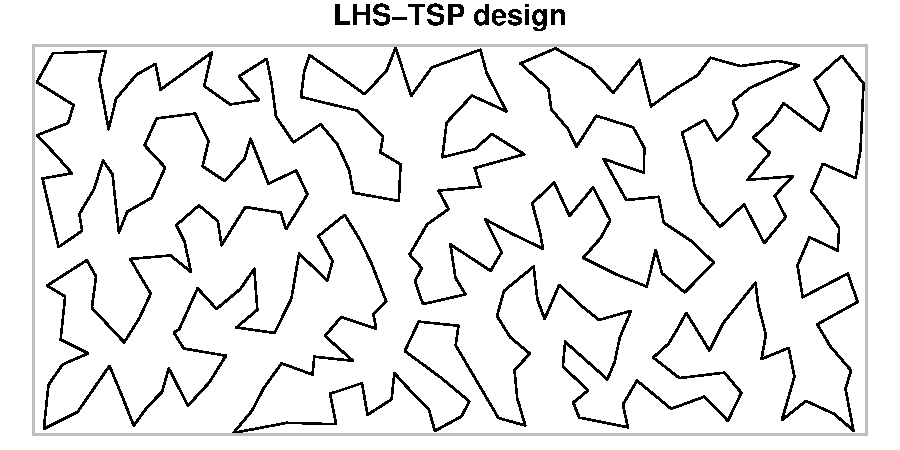
\includegraphics[width=2.5in]{../graphics/LHS-TSP000161.pdf}
\caption{Shortest path through a LHS design}
\label{lhstsp000161}
\end{subfigure}
\begin{subfigure}{2.5in}
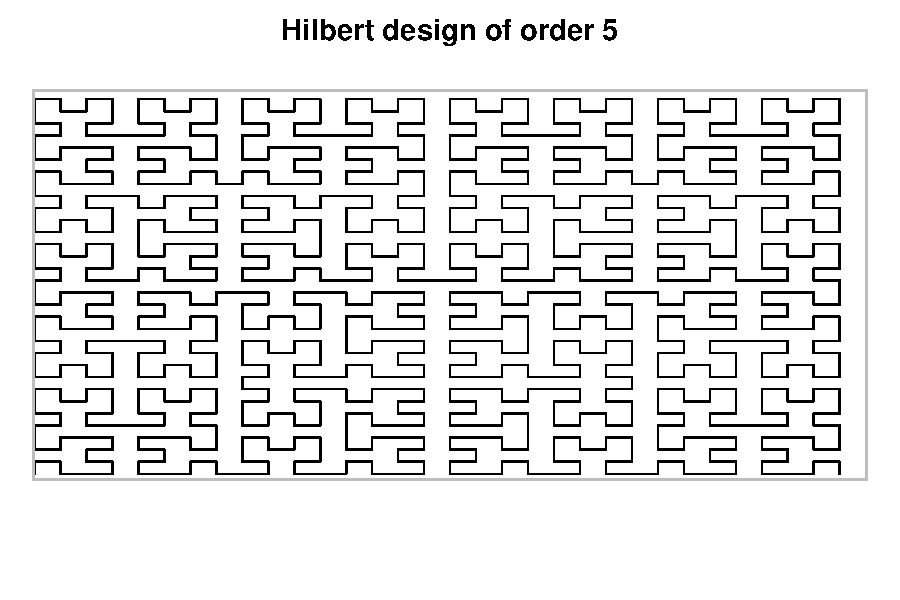
\includegraphics[width=2.5in]{../graphics/Hilbert000237.pdf}
\caption{Space-filling Hilbert design, more refined}
\label{hilbert000237}
\end{subfigure}

\caption{Examples of plans from six design schemes. Except for the Hilbert
curve of order 5, all of these plans have approximately the same total length.}
\label{plancomparison}
\end{figure}


\subsubsection{Parallel serpentine transects}

One simple way to observe a greater variety of locations and different
directions is to add lateral ``zigzags'' to line transects. We include
alternate right and left turns at right angles to create serpentine transects.
This could decrease prediction variance because more of the path will be close
to each point in the study area than would be under a line transect design with
similar total distance. They will also improve estimation of the covariance
function in the presence of anisotropy. Figure~\ref{plancomparison}, top right,
shows two examples.
% Note: Serp has higher average and max distance from path than Sys but lower
% than SRS and Inhib.

% What to do with the comments about anisotropy? Consolidate them and put them
% in one spot? Anisotropic models are rarely used (underused) and we are
% simulating from isotropic models, but "go in more than one direction if you
% have anisotropic data" is advice worth spending a paragraph on.


\subsubsection{Latin hypercube sampling}

Random Latin hypercube sampling (LHS) produces a design that spreads discrete
points through a (potentially high-dimensional) design space, ensuring that
the full range of each dimension is included while remaining balanced and
keeping the number of points small~\citep{mckayetal}. This is done by
partitioning each dimension into a specified number \(k\) of intervals (thus
stratifying a \(d\)-dimensional design space into \(k^{d}\) cells), selecting
a Latin hypercube design to determine which \(k\) cells will contain a design
point, and then drawing each design point from a uniform distribution over its
cell. In two dimensions, this scheme produces point designs with good spatial
coverage properties. We use the LHS design as waypoints for a path. Because
longer distance typically brings increased costs, we treat this as a traveling
salesperson problem (TSP) and use the shortest path through the waypoints as
our design. This LHS-TSP scheme produces paths that have many sharp corners but
leaves few large voids (example in Figure~\ref{plancomparison}, bottom left).
Waypoints are generated by the \texttt{lhs} R package~\citep{lhs} and connected
into a shortest path by the \texttt{TSP} package~\citep{tsp}. A downside of
this design scheme is that the length cannot be specified directly, and only
certain distances are possible depending on the number of bins used.


\subsubsection{Space-filling curves}

As a representative of space-filling curves, we use the Hilbert curve scaled
to fit the study site. These designs have many short segments meeting at right
angles. The only parameter of this design scheme is the order, or number of
iterations used in refining the curve. Each iteration increases the length and
complexity of the design. This is produces a deterministic design, so a random
offset is added to vary which locations are visited. The Hilbert curve is
generated by the \texttt{HilbertVis} R package~\citep{hilbertvis}.

%\paragraph{Particle movement model}
%Models the way data are actually collected. Waypoints generated sequentially by
%generating a jump distance and a direction. The jump distance is generated from
%a scaled beta distribution, and negatively correlated with previous jump
%distance. This behavior should approximately alternate between a short
%``transition'' and a long transect. The negative correlation was achieved by
%applying a \(1 - x\) transformation to a beta autoregressive
%process~\citep{mckenzie}. The direction angle is drawn from a bimodal
%distribution that is symmetric around 0 (a normal distribution reflected about
%0). {\it explain the Strauss part}

%{\it set up to think about adaptive sampling (adding a transect at a time or
%stopping early but don't actually do it here)}


\subsubsection{Spatial coverage criterion}

One critically important characteristic of a spatial design is the concept of
spatial coverage, or how well the design represents the study site in the sense
that all points in the site are close to observed locations. The criterion we
propose to measure this is the average distance to the path. We define the
distance between a point and the path as the distance between that point and
the nearest point on the path, then take the average over all points in the
study region. This can be roughly understood as the radius of a typical
unsurveyed void.


\subsection{LGCP model and notation}

The full point process is denoted \(\mathbf{X}\) and operates over the entire
study site \(\mathcal{R}\). The full realized point pattern is denoted
\(\mathbf{x}\) and is a finite (countable) subset of \(\mathbf{R}\). However,
only a subregion of \(\mathcal{R}\) is surveyed. This subregion is
\(\mathcal{S}\), the set of all points within a specified radius of the survey
path. The observed point pattern is defined as
\(\mathbf{x}_{\mathcal{S}} = \mathbf{x} \cap \mathcal{S}\).

In the LGCP model, \(\mathbf{X}\) is a Poisson process with intensity
function \(\lambda(u)\), \(u \in \mathcal{R}\). This intensity function is
itself a stochastic process, modeled on the natural logarithm scale as
\begin{equation}
\log[\lambda(u)] = \mu + \mathbf{e}(u),
\end{equation}
with an intercept \(\mu\) and spatial error term \(\mathbf{e}(u)\). The error
term is a Gaussian process with mean 0 and covariance function \(C(u, v)\).
In our simulation study, \(C\) is a stationary and isotropic Mat\'{e}rn
covariance function with smoothness parameter \(\nu\), spatial scale \(\rho\),
and variance \(\sigma^{2}\).


\subsubsection{Model-based criteria}

For model-based comparisons, we compare the posterior distribution of the
intercept \(\mu\) to the realized mean of the simulated GP, and evaluate two
spatial prediction criteria. For the intercept, we simply record whether the
95\% central interval captures the realized mean. This is aggregated into the
capture rate for the design scheme.

The spatial prediction criteria that we evaluate are the mean squared
prediction error (MSPE) of the log intensity surface,
\begin{equation}
\mathrm{E}[(\mu + \mathbf{e}(u) - \log[\lambda(u)]^{2}|\mathbf{x}_{\mathcal{S}}],
\end{equation}
and the average prediction variance (APV) of the latent Gaussian process,
\begin{equation}
\mathrm{Var}[\mathbf{e}(u)|\mathbf{x}_{\mathcal{S}}].
\end{equation}
In the above notation, \(\lambda\) is the true realized intensity function,
which is known in the simulations.

The capture rate of the mean describes accuracy in the overall scale of the
intensity surface. Inaccuracy in the mean implies that that model will predict
overall too many or too few events. The other criteria reflect two important
characteristics of a useful spatial prediction. First, deviation from the true
surface should be low, and is indicated by low MSPE. Second, the model's own
assessment of prediction uncertainty will be used in practice to build trust in
the inferences, so low APV is desirable. 


\subsubsection{Model fitting}

We fit the spatial LGCP model using nested integrated Laplace approximations
and the R-INLA package~\citep{rueetal,rinla}. We use the \texttt{inla()}
function with its default optimizer parameters. The Gaussian process is
approximated using a finite element approach \citep{lindgrenetal}. The finite
element approach models the GP at a finite set of nodes in a mesh, and requires
an assumption that the realized GP surface is approximately linear between the
nodes. The data analyst must choose the nodes so that this assumption holds.
Then, the point pattern is modeled by pseudodata placed at the events and the
finite element nodes~\citep{simpsonetal}. When using an adequate finite element
mesh, this procedure allows fast and accurate approximation of the posterior
distribution.%~\citep{flagghoegh}.


\section{Simulation study}

We compare the design schemes by applying multiple designs from each scheme
to the same simulated datasets. There are two data-generating models and five
datasets generated from each, for a total of ten datasets
(Section \ref{simsite}). We will focus on two illustrative datasets when
presenting the results. We use 8 schemes at four levels of survey effort, and
100 designs generated from each scheme at each effort level
(Section \ref{simschemes}). All events within a 2 unit radius of the path are
observed. The same model is fit to each observed point pattern
(Section \ref{simmodel}).



\subsection{Study site}
\label{simsite}

\begin{figure}

\begin{subfigure}{5in}
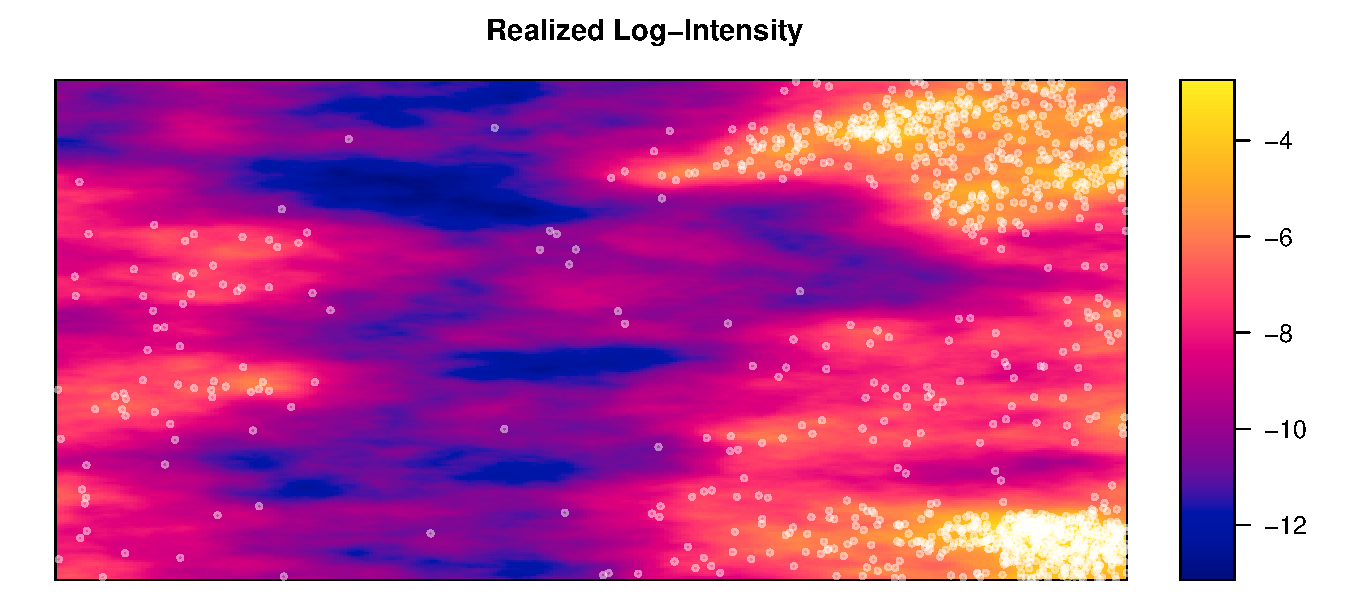
\includegraphics[width=5in]{../graphics/lambda-LGCP000004.pdf}
\caption{Realized LGCP log-intensity}
\label{lambdalgcp}
\end{subfigure}

\begin{subfigure}{5in}
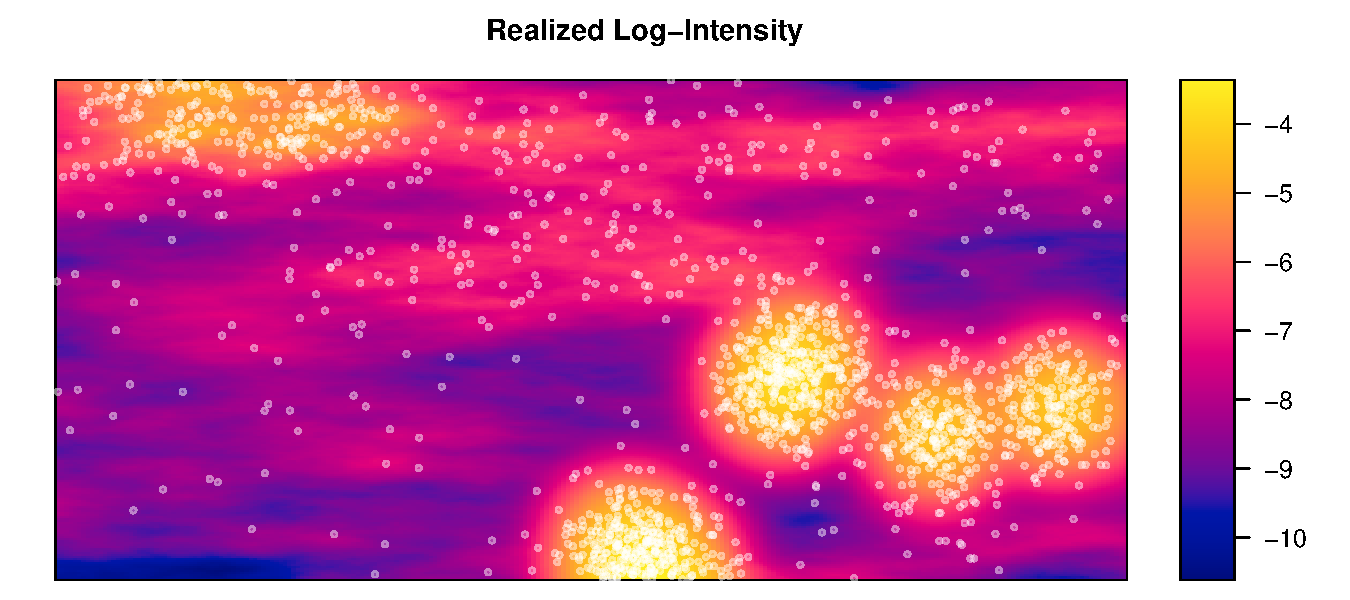
\includegraphics[width=5in]{../graphics/lambda-Cluster000004.pdf}
\caption{Realized LGCP with Clusters log-intensity}
\label{lambdacluster}
\end{subfigure}

\caption{The realized intensity function (natural log scale) and complete
point pattern from a LGCP, and from a LGCP superposed with a cluster process.}
\label{fulldata}
\end{figure}

We consider a fictitious site \(\mathcal{R}\) with the simple shape of a 1500
unit by 700 unit rectangle. In this site, we simulate two data generating
models that produce random intensity functions with hotspots. First, a LGCP
with latent GP mean \(\mu = \log(250 / |\mathcal{R}|) = -8.34\) and
Mat\'{e}rn covariance function with \(\nu = 1\), \(\sigma = 2\), and
\(\rho = 200\). This model produces relatively unstructured hotspots due to
large variability in the GP. Figure \ref{lambdalgcp} shows an example
realization from this process.

Second, a two-stage cluster process and a LGCP are superposed. The cluster
process (a Neyman-Scott or, more specifically, Thomas process) is constructed
as follows. The number of clusters is Poisson-distributed with mean 3. The
number of events per cluster is Poisson-distributed with mean 200. The cluster
centers are distributed uniformly over \(\mathcal{R}\). Events come from a
bivariate normal distribution with mean equal to the cluster center and
variance \(\boldsymbol{\Sigma} = \tau^{2}\mathbf{I}\), \(\tau = 50\). The LGCP
component has \(\mu = \log(250 / |\mathcal{R}|) = -8.34\) and Mat\'{e}rn
covariance with \(\nu = 1\), \(\sigma = 1\), and \(\rho = 200\). This model is
based upon the typical conceptual model of a firing range, with a background
process (represented by the LGCP) and a small number of higher-intensity
foreground clusters containing the events of interest (example in Figure
\ref{lambdacluster}). As a shorthand, we refer to this generative process as
LGCP with Clusters.

The LGCP generating process matches the model fit to the realized data. The
model should both produce accurate predictions and have low bias in the
posterior means of the parameters. On the other hand, the parameters of the
LGCP with Clusters process will not correspond to the LGCP model parameters,
but we anticipate that in general the latent GP in the LGCP model will still
accurately predict the log-intensity function.


\subsection{Path design schemes}
\label{simschemes}

\begin{table}
\caption{Design schemes used in the simulation study. The table presents the
design parameters, distance travelled along the path, percent of the study area
surveyed, and average distance to the path under each of four survey effort
levels. The average distance to the path varies from design to design, and is
presented as average (SD).\\
* Variable area due to overlapping segments, reported as average (SD).\\
** Variable distance surveyed, reported as average (SD).}
\label{designtable}
\tiny
\begin{tabular}{|l|c|c|c|c|}
\hline
Scheme & Low Effort & Medium Effort & High Effort & Very High Effort \\
\hline
SRS & 10 transects & 25 transects & 50 transects & 70 transects \\
\hfill\emph{Length:} & 7000 units & 17500 units & 35000 units & 49000 units \\
\hfill\emph{\% Surveyed:} & 2.65\% (0.0618\%)* & 6.46\% (0.202\%)* & 12.5\% (0.331\%)* & 17.2\% (0.459\%)* \\
\hfill\emph{Avg. Dist. to Path:} & 73.7 (16.4) & 29.7 (6.01) & 15.0 (1.99) & 10.8 (1.44) \\
\hline
Systematic & 10 transects & 25 transects & 50 transects & 70 transects \\
\hfill\emph{Length:} & 7000 units & 17500 units & 35000 units & 49000 units \\
\hfill\emph{\% Surveyed:} & 2.68\% & 6.70\% & 13.4\% & 18.7\% \\
\hfill\emph{Avg. Dist. to Path:} & 38.4 (0.866) & 15.2 (0.181) & 7.56 (0.0307) & 5.40 (0.0164) \\
\hline
Inhibitory, & 9 transects & 23 transects & 45 transects & 63 transects \\
10\% Close Pairs & 1 paired & 2 paired & 5 paired & 7 paired \\
\hfill\emph{Length:} & 7000 units & 17500 units & 35000 units & 49000 units \\
\hfill\emph{\% Surveyed:} & 2.66\% (0.0582\%)* & 6.53\% (0.172\%)* & 12.8\% (0.314\%)* & 17.5\% (0.427\%)* \\
\hfill\emph{Avg. Dist. to Path:} & 50.3 (5.35) & 20.8 (1.82) & 10.6 (1.24) & 7.64 (0.576) \\
\hline
Inhibitory, & 8 transects & 20 transects & 40 transects & 56 transects \\
20\% Close Pairs & 2 paired & 5 paired & 10 paired & 14 paired \\
\hfill\emph{Length:} & 7000 units & 17500 units & 35000 units & 49000 units \\
\hfill\emph{\% Surveyed:} & 2.67\% (0.0444\%)* & 6.56\% (0.157\%)* & 12.8\% (0.303\%)* & 17.6\% (0.368\%)* \\
\hfill\emph{Avg. Dist. to Path:} & 53.5 (8.37) & 22.0 (2.97) & 11.4 (1.70) & 8.26 (0.826) \\
\hline
Serpentine, & 7 transects & 22 transects & 47 transects & 67 transects \\
5 Zigzags & 75 unit offset & 23.9 unit offset & 11.2 unit offset & 7.84 unit offset \\
\hfill\emph{Length:} & 7000 units & 17500 units & 35000 units & 49000 units \\
\hfill\emph{\% Surveyed:} & 2.67\% & 6.68\% & 13.4\% & 18.7\% \\
\hfill\emph{Avg. Dist. to Path:} & 43.2 (1.83) & 16.0 (0.215) & 7.79 (0.0508) & 5.51 (0.0309) \\
\hline
Serpentine, & 7 transects & 22 transects & 47 transects & 67 transects \\
8 Zigzags & 42.9 unit offset & 13.6 unit offset & 6.38 unit offset & 4.48 unit offset \\
\hfill\emph{Length:} & 7000 units & 17500 units & 35000 units & 49000 units \\
\hfill\emph{\% Surveyed:} & 2.67\% & 6.67\% & 13.3\% & 18.7\% \\
\hfill\emph{Avg. Dist. to Path:} & 44.5 (2.03) & 15.9 (0.169) & 7.76 (0.0328) & 5.50 (0.0271) \\
\hline
LHS-TSP & 50 bins & 300 bins & 1200 bins & 2400 bins \\
\hfill\emph{Length:} & 7177 (189) units** & 17191 (168) units** & 34196 (225) units** & 48433 (342) units** \\
\hfill\emph{\% Surveyed:} & 2.73\% (0.0722\%)** & 6.51\% (0.0632\%)** & 12.9\% (0.0835\%)** & 18.2\% (0.127\%)** \\
\hfill\emph{Avg. Dist. to Path:} & 43.5 (1.44) & 17.4 (0.186) & 8.63 (0.0683) & 6.08 (0.0562) \\
\hline
Hilbert Curve & 3rd Order & 4th Order & 5th Order & 6th Order \\
\hfill\emph{Length:} & 8581 units & 17442 units & 35025 units & 70121 units \\
\hfill\emph{\% Surveyed:} & 3.27\% & 6.634\% & 13.3\% & 26.47\% \\
\hfill\emph{Avg. Dist. to Path:} & 37.3 (1.95) & 17.9 (0.480) & 8.77 (0.113) & 4.37 (0.0382) \\
\hline
\end{tabular}
\end{table}

The simulation uses each of the design schemes discussed in
Section~\ref{methodschemes}. The surveyed region \(\mathcal{S}\) consists of
all points within 2 units of the design. That is, \(\mathcal{S}\) is a
collection of strips along each segment of the design. All events within 2
units of the design are observed and all events farther than 2 units from
the path are unobservable.

The design parameters for each scheme are varied to create four different
levels of survey effort: low, medium, high, and very high. Within each effort
level, the total length or distance traveled is comparable across all schemes.
The inhibitory plus close pairs scheme and the serpentine scheme are further
varied to employ different numbers of pairs and different numbers of zigzags,
respectively. Table \ref{designtable} provides an overview of the different
settings.

The parallel line transect schemes have transects running north-south, with
the effort level determining the number of transects. We expect the simple
random sample scheme to produce high prediction variance and large prediction
error in big gaps between transects. The systematic sample scheme uses a
uniformly-distributed starting point and constant spacing between adjacent
transects. We expect systematic transects to provide accurate inferences for
the intensity surface and moderate prediction variance.% However, this scheme
%can miss structures at certain sizes because no transects are close to each
%other in the east-west direction.

For the inhibitory plus close pairs line transect scheme, we vary the numbers of
paired and unpaired transects. The total number of transects is the same as in
the SRS and systematic designs, but 10\% and 20\% of the transects (rounded to
the nearest integer) are designated as redundant members of a pair. The
remaining primary transects are placed according to a one-dimensional Strauss
process \citep{strauss,kellyripley}. The Strauss attraction parameter is set
at \(\gamma = 0.05\) and the radius for counting pairs is 1500 units divided
by the total number of transects. Then each redundant transect is randomly
paired to a primary transect, and placed within the pair radius of the primary
transect according to a uniform distribution. We expect this scheme to have
intermediate performance between the simple random sample and the systematic
line transect schemes.

The serpentine transect scheme has transects running north-south with constant
east-west spacing and a random starting point for the first transect. The
number of zigzags (north-south segments) is 5 or 8 per transect. The designs
are constructed to have the same length as the line-transect designs: there are
three fewer serpentine transects, and the perpendicular offset is set so the
total east-west distance equals the length of three north-south line transects.
These designs should result in smaller prediction errors and lower variance
farther from the path when compared to line-transect designs.

Our Latin hypercube sampling/traveling salesperson (LHS-TSP) scheme uses a
different number of bins for each effort level (see Table \ref{designtable}).
Preliminary experimentation found that these bin numbers produced total lengths
similar to the transect schemes. The LHS-TSP scheme is expected to result
in small prediction errors and low prediction variance per unit distance
traveled. However, the designs will have many sharp corners and, on rare
occasions, some large voids.

The Hilbert curve scheme uses a random starting point and a Hilbert curve of
order 3, 4, 5, or 6. The path length is a deterministic function of the order
and differs greatly among curves of different orders. These orders yield
lengths similar to the lengths of the transect designs. Hilbert designs should
provide low prediction variance, but have lots of short segments.


\subsection{Model specification}
\label{simmodel}

The same Bayesian LGCP model is fit to each observed dataset. The observed
point pattern \(\mathbf{x}_{\mathcal{S}}\) is a partial realization of
\(\mathbf{X}\), a Poisson process on \(\mathcal{R}\) with intensity
\(\lambda(u)\). The intensity is modeled as
\(\log[\lambda(u)] = \mu + \mathbf{e}(u)\). The spatial error term
\(\mathbf{e}\) is a Gaussian process with mean \(\mathbf{0}\) and a
Mat\'{e}rn covariance function with fixed \(\nu = 1\).
% Remember alpha = nu + d/2 so alpha = 2 and d = 2 imply nu = 1.

The intercept \(\mu\) has a \(\mathrm{Unif}(-\infty, \infty)\) prior.
% Or \(\mathrm{N}(0, \infty)\)?
The covariance parameters \(\sigma\) and \(\rho\) have a PC prior with
\(\mathrm{Pr}(\sigma > 3) = 0.1\) and \(\mathrm{Pr}(\rho < 100) = 0.1\)
\citep{fuglstadetal,simpsonpc}.


\subsection{Finite element mesh}
\label{simmesh}

The Gaussian process prediction surface is approximated on the finite element
mesh shown in Figure~\ref{meshfull}. The GP is predicted at the 298 nodes
(black dots on the plot) and is linearly interpolated elsewhere. The nodes are
weighted according to the area of their dual cells (grey outlines) and used
for numerical integration of the likelihood \citep{lindgrenetal}.

The choice of mesh is important because a mesh that is too coarse cannot
represent small-scale structures and thus will incur large approximation
errors. On the other hand, the mesh has implications for computation because
the nodes and the observed events correspond to pseudodata points. In our
sparsely-observed point pattern setting, the number of mesh nodes will be
large relative to the number of observed events, making the mesh the primary
driver of computational complexity in fitting the model.

A good approach in practice is to refit the model with several meshes and
refine the mesh until the prediction surface has converged. However, for a
simulation study we must choose one mesh that will perform reasonably well for
a wide variety of datasets. This mesh is adequately fine to model the
large-scale trends in the surface while keeping the computing time well under
a minute for each model fit.
% Finer meshes fit to the best-performing design don't result in more detailed
% surfaces. This mesh can represent the surface with as much detail as these
% designs can contain. Add some comments on how we have to keep it fixed for
% the simulations but users should so sensitivity analysis.

\begin{figure}
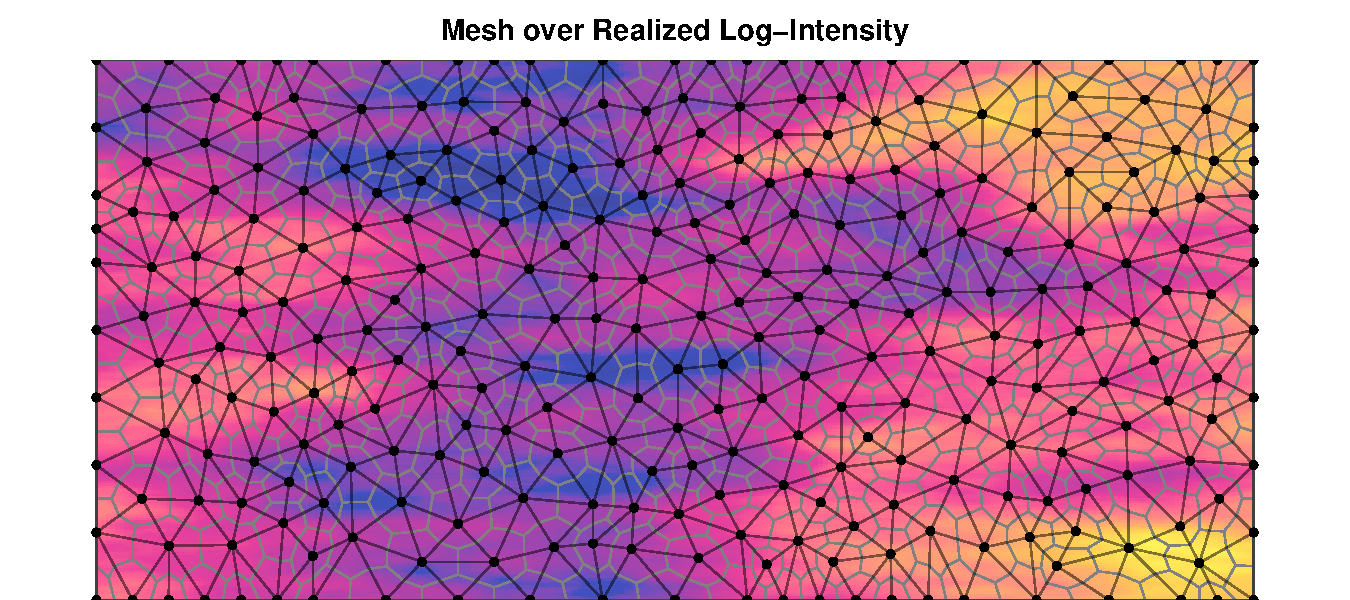
\includegraphics[width=5in]{../graphics/mesh-LGCP000004.pdf}
\caption{Illustration of the mesh used to approximate the latent GP. The mesh
nodes are used in a numerical integration scheme where they are weighted by the
area of their dual cells (outlined in grey).}
\label{meshfull}
\end{figure}


%\section{Theory/calculation}
% A Theory section should extend, not repeat, the background to the article already dealt with in the Introduction and lay the foundation for further work. In contrast, a Calculation section represents a practical development from a theoretical basis.


\section{Results}

%\subsection{Initial Observations}

In describing the results, we focus on one LGCP dataset and one LGCP with
Clusters dataset (Figure~\ref{fulldata}). The results are similar for all
datasets (see figures in \ref{profplots}). These two datasets were chosen for
illustration because the simulations using them exhibited a wide variety of
outcomes. This included a mix of very good and very poor prediction
performance.

\begin{figure}

\begin{subfigure}{5in}
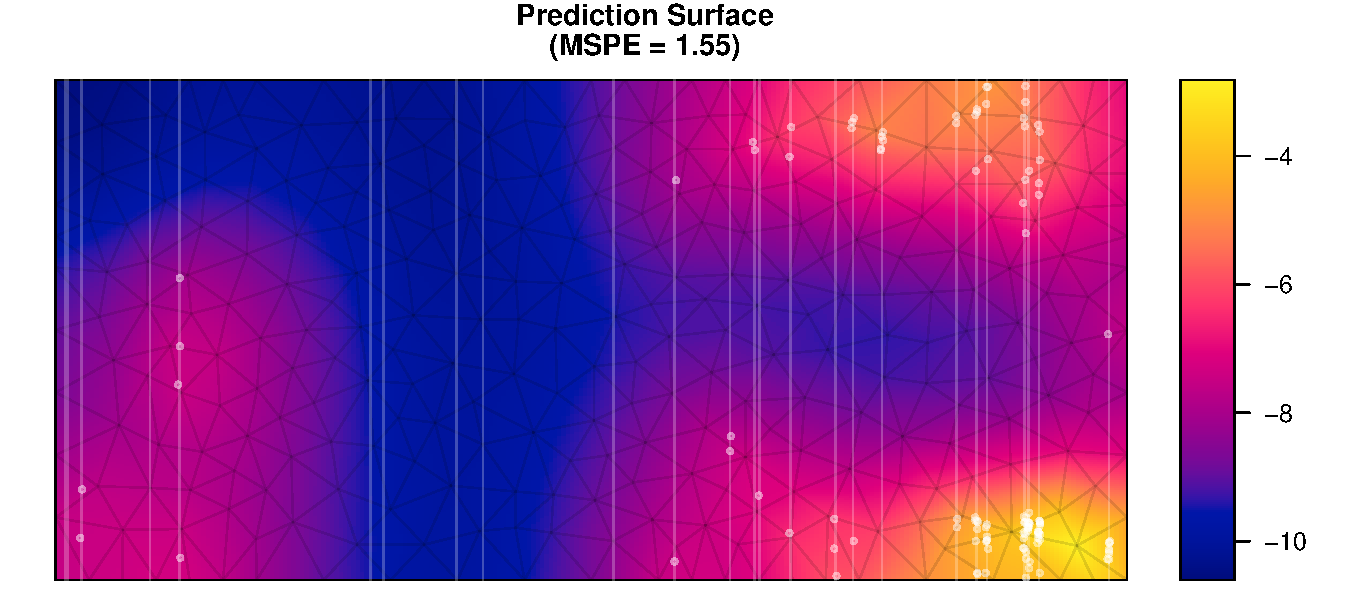
\includegraphics[width=5in]{../graphics/lambda-SRS000187-LGCP000004.pdf}
\caption{Predicted log-intensity}
\label{lambdasrs000187lgcp}
\end{subfigure}

\begin{subfigure}{5in}
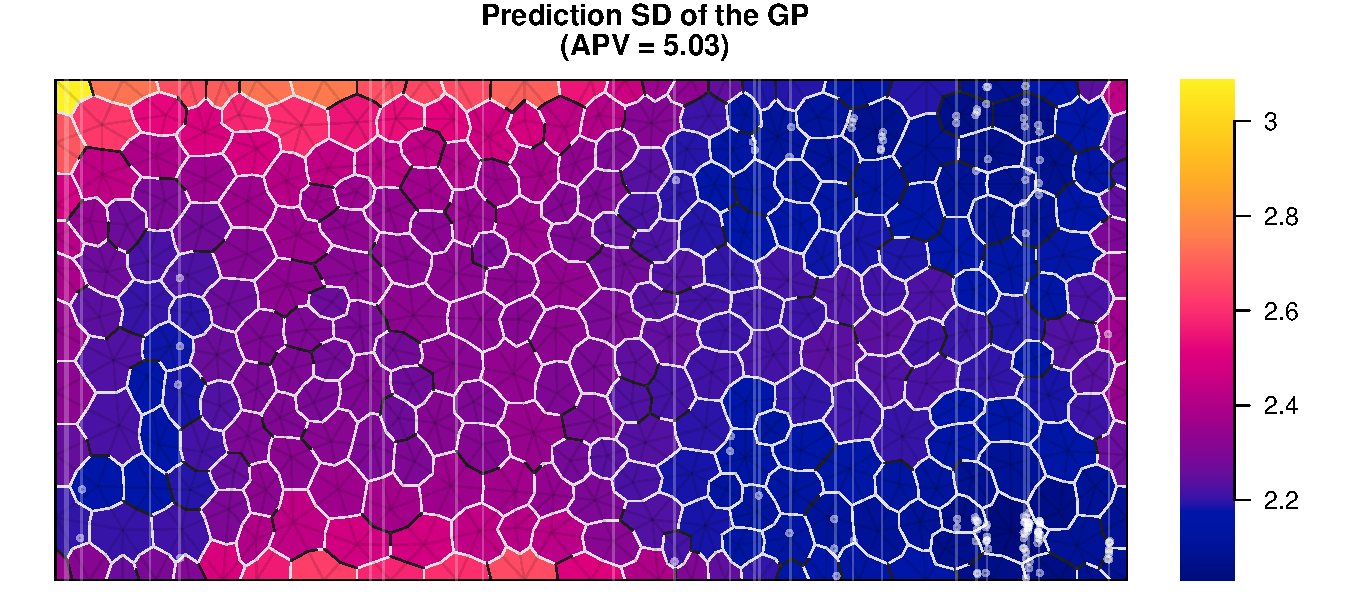
\includegraphics[width=5in]{../graphics/lambdaSD-SRS000187-LGCP000004.pdf}
\caption{Prediction SD}
\label{sdsrs000187lgcp}
\end{subfigure}

\caption{Predicted log-intensity function and prediction standard deviation
using data observed via a SRS of line transects. The SD is shown for each
finite element node. This example is a medium-effort plan applied to a
LGCP dataset.}
\label{srs000187lgcp}
\end{figure}

Figure~\ref{srs000187lgcp} shows an example where the model does well at
predicting the intensity of the realized LGCP. This example uses one of the
SRS paths. In the figure, the path appears in white and the observed events
are shown as white dots. The posterior predicted mean of the log-intensity
(top panel) accurately captures the large-scale features, but smooths out much
of the small-scale variation. The bottom panel shows the prediction standard
deviation for each mesh node. The SD ranges from 2.0 to 3.1, and is lowest
near observed events. SD increases farther from observed events, including
in places where the surveyed area was observed to contain no events.

This same survey plan also did well for the LGCP with Clusters dataset, with
the model accurately capturing the large-scale details of the intensity
function, including two of the circular hotspots corresponding to clusters
(Figure \ref{lambdasrs000187clust}). However, it also smoothed the surface
quite a bit, notably merging the two overlapping clusters into a single oblong
hotspot.

\begin{figure}

\begin{subfigure}{5in}
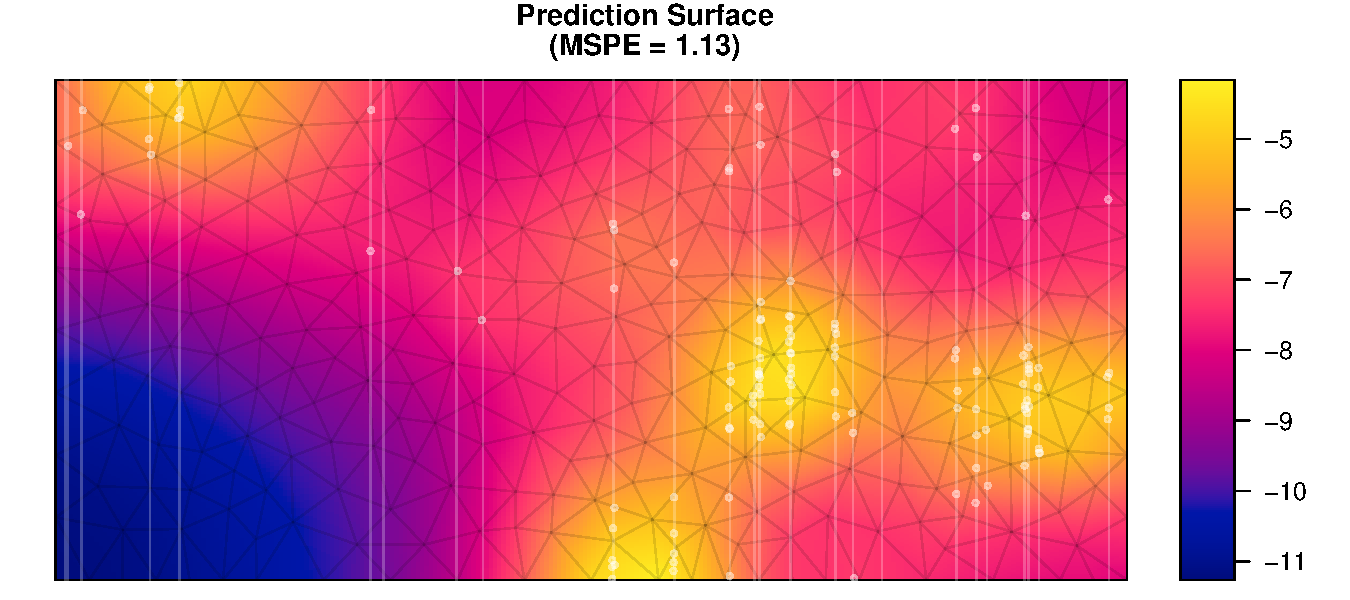
\includegraphics[width=5in]{../graphics/lambda-SRS000187-Cluster000004.pdf}
\caption{Predicted log-intensity}
\label{lambdasrs000187clust}
\end{subfigure}

\begin{subfigure}{5in}
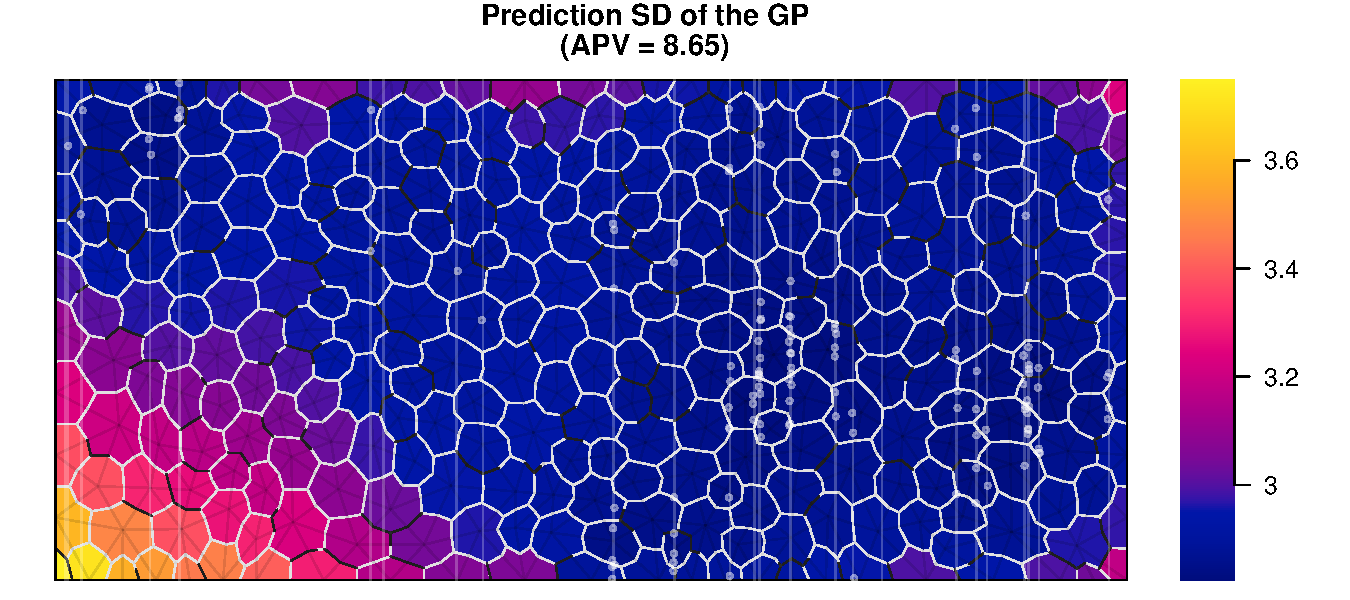
\includegraphics[width=5in]{../graphics/lambdaSD-SRS000187-Cluster000004.pdf}
\caption{Prediction SD}
\label{sdsrs000187clust}
\end{subfigure}

\caption{Predicted log-intensity function and prediction standard deviation
using data observed via a SRS of line transects. The SD is shown for each
finite element node. This example is a medium-effort plan applied to a
LGCP with Clusters dataset.}
\label{srs000187clust}
\end{figure}

Most plans yielded similar prediction surfaces, capturing the large-scale
trends, and having the least uncertainty near observed events. Results varied
in accuracy at the most extreme peaks and valleys of the intensity function and
in overall SD across the study region.

However, a small number of model fits failed to converge, and others suffered
from apparent edge effects.
% Usually, but not always, on the boundary. Sometimes on a peninsula.
For example, Figure~\ref{serp000148} shows the prediction surface resulting
from a serpentine transect plan. The predicted log-intensity has a hotspot of
extremely large values in the southeast corner (notice the color scale). The
hotspot is driven by two nodes on the boundary with very large prediction
values. Another, less extreme, edge effect is present in the northeast corner.
The surface also contains many circular peaks centered on observed events.
When computational problems occur, they may be fixed by refining the mesh at
additional computational cost. We were not able to use a finer mesh for all
simulations due to computational limitations, but we point out which schemes
are robust to these problems (see Tables \ref{lgcptable} and \ref{clusttable}).

Section~\ref{compissues} illustrates refitting the model using a refined mesh.
The sections after that compare the schemes in terms of model-based criteria
applied to one realized LGCP dataset and one realized LGCP with Clusters
dataset, and then discuss the results in the context of spatial coverage.

\begin{figure}

\begin{subfigure}{5in}
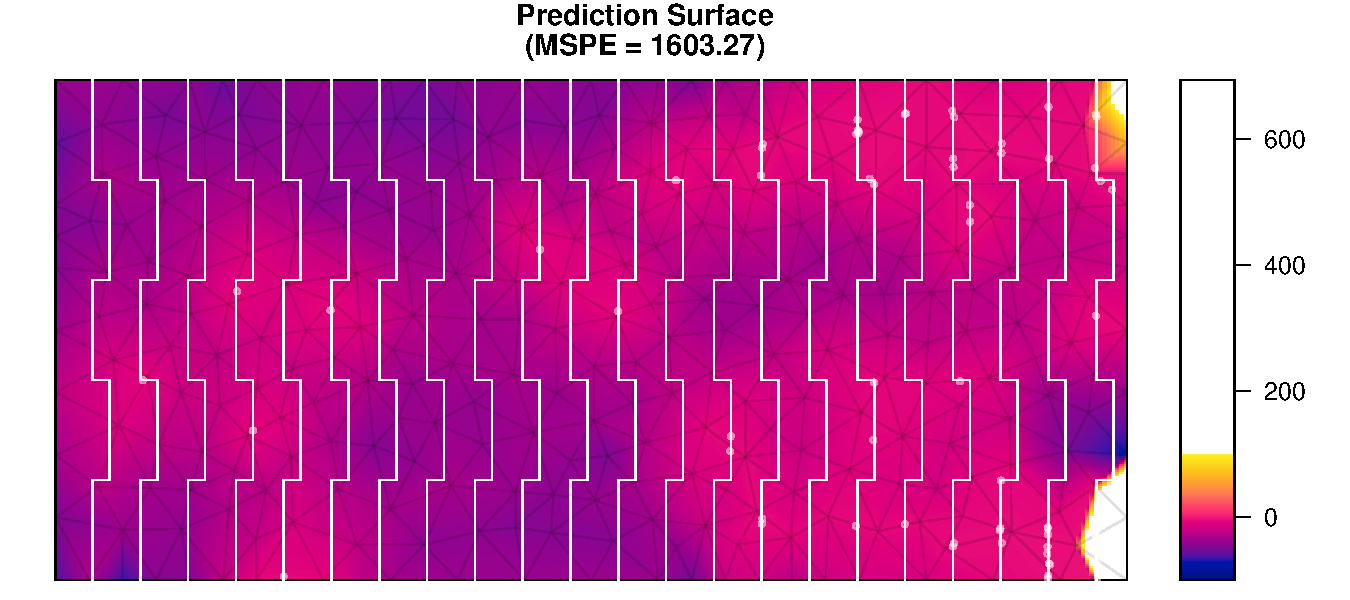
\includegraphics[width=5in]{../graphics/lambda-Serp000148-LGCP000004.pdf}
\caption{Predicted log-intensity. The color scale is truncated at 100, but
reaches a maximum of 692.}
\label{lambdaserp000148lgcp}
\end{subfigure}

\begin{subfigure}{5in}
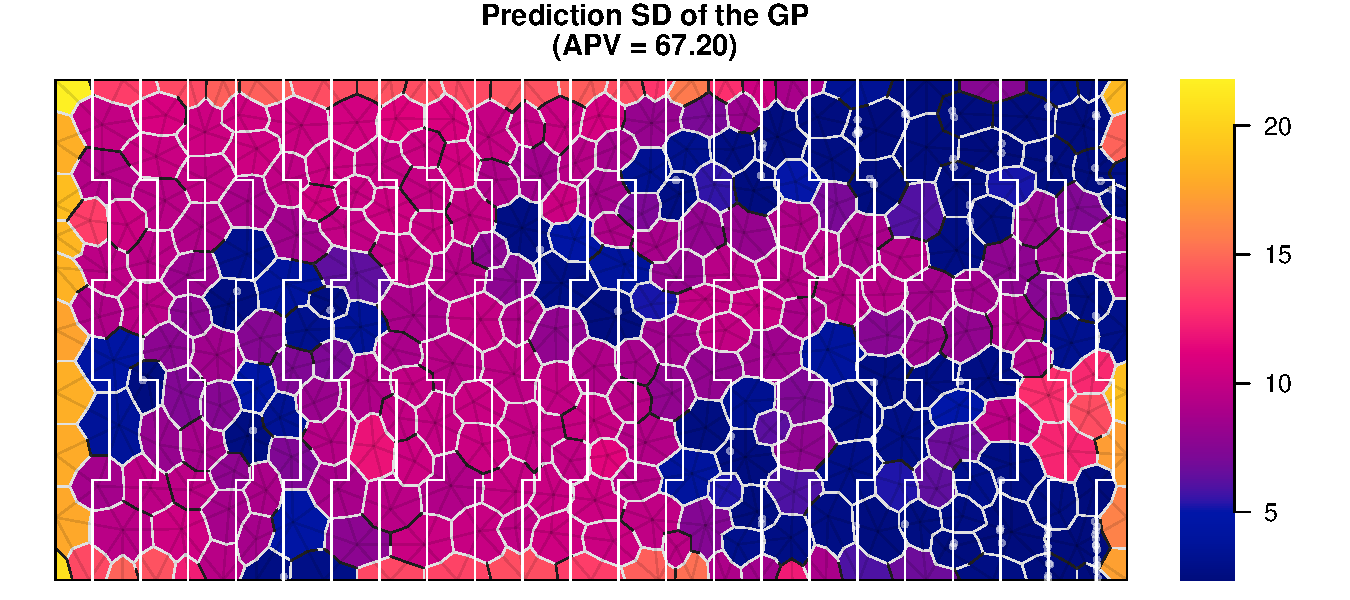
\includegraphics[width=5in]{../graphics/lambdaSD-Serp000148-LGCP000004.pdf}
\caption{Prediction SD}
\label{sdserp000148lgcp}
\end{subfigure}

\caption{Predicted GP surface and prediction SD using data observed via a
serpentine transect plan. The prediction has an apparent edge effect in the
southeastern corner. The SD is high across much of the site. This example is
a medium-effort plan applied to a LGCP dataset.}
\label{serp000148}
\end{figure}


\begin{figure}

\begin{subfigure}{4.5in}
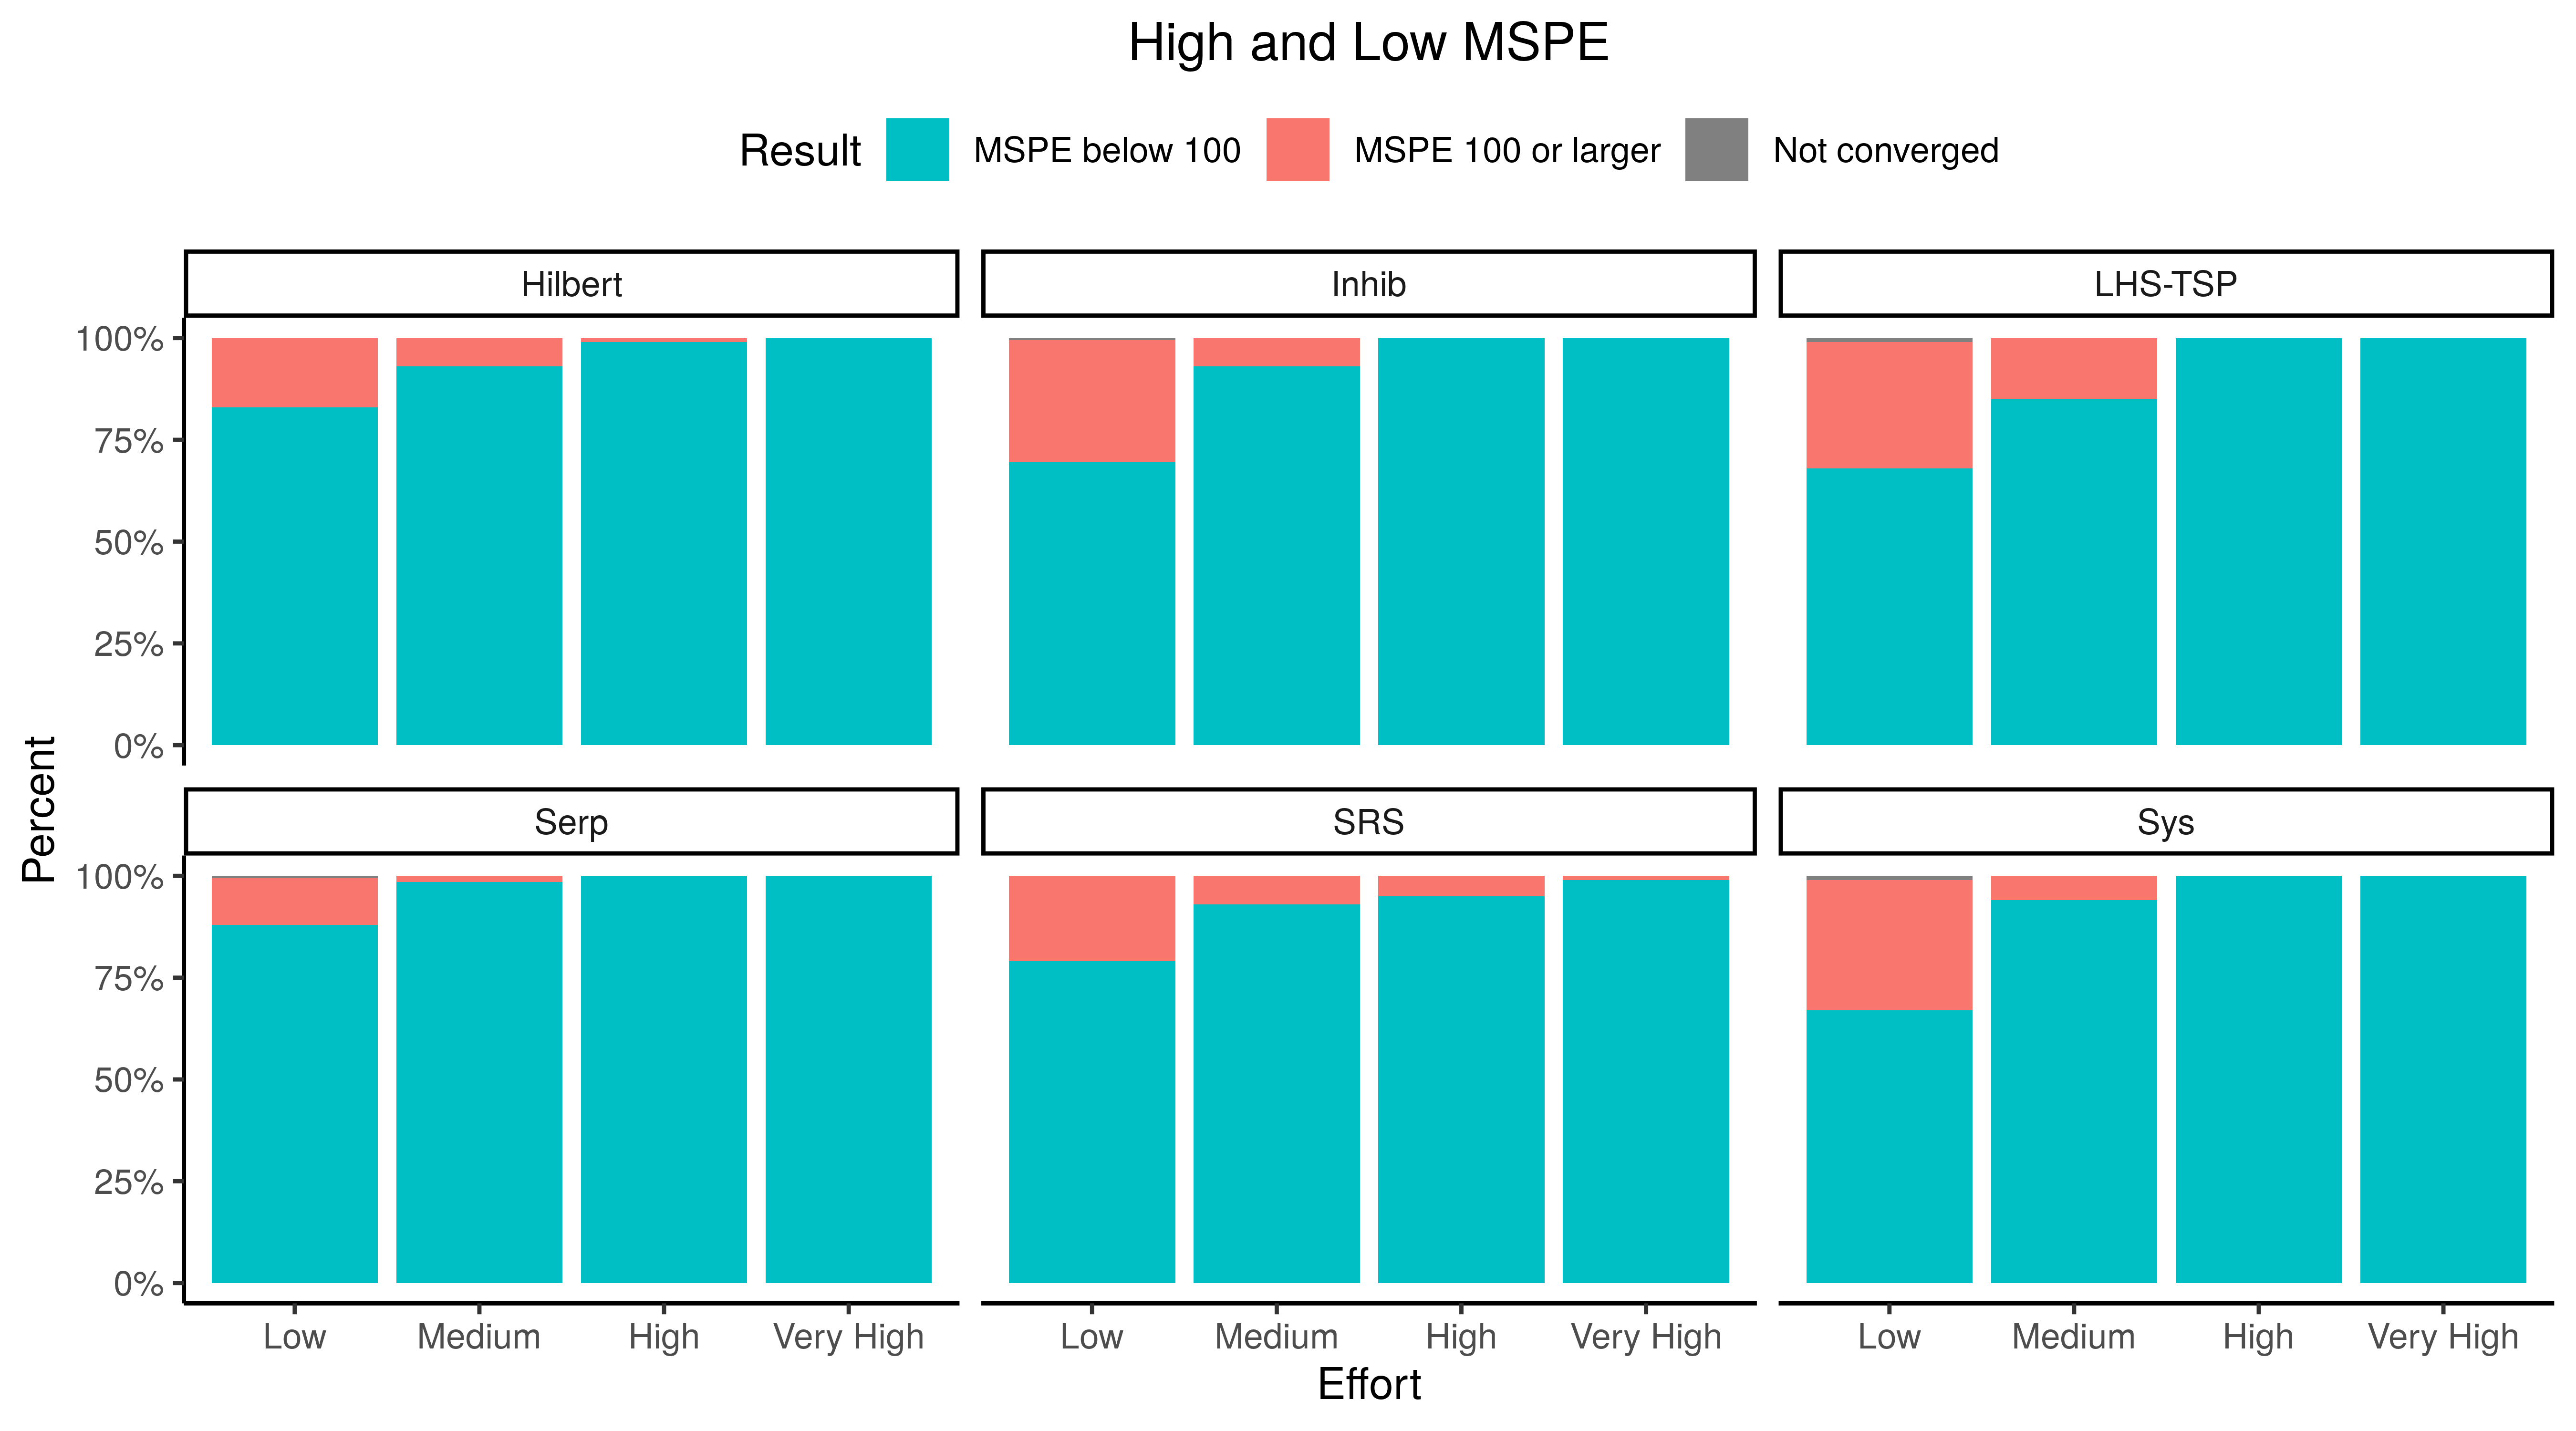
\includegraphics[width=4.5in]{../graphics/HighMSPE-LGCP000004.png}
\caption{MSPE distribution for one LGCP dataset}
\label{highmspelgcp}
\end{subfigure}

\begin{subfigure}{4.5in}
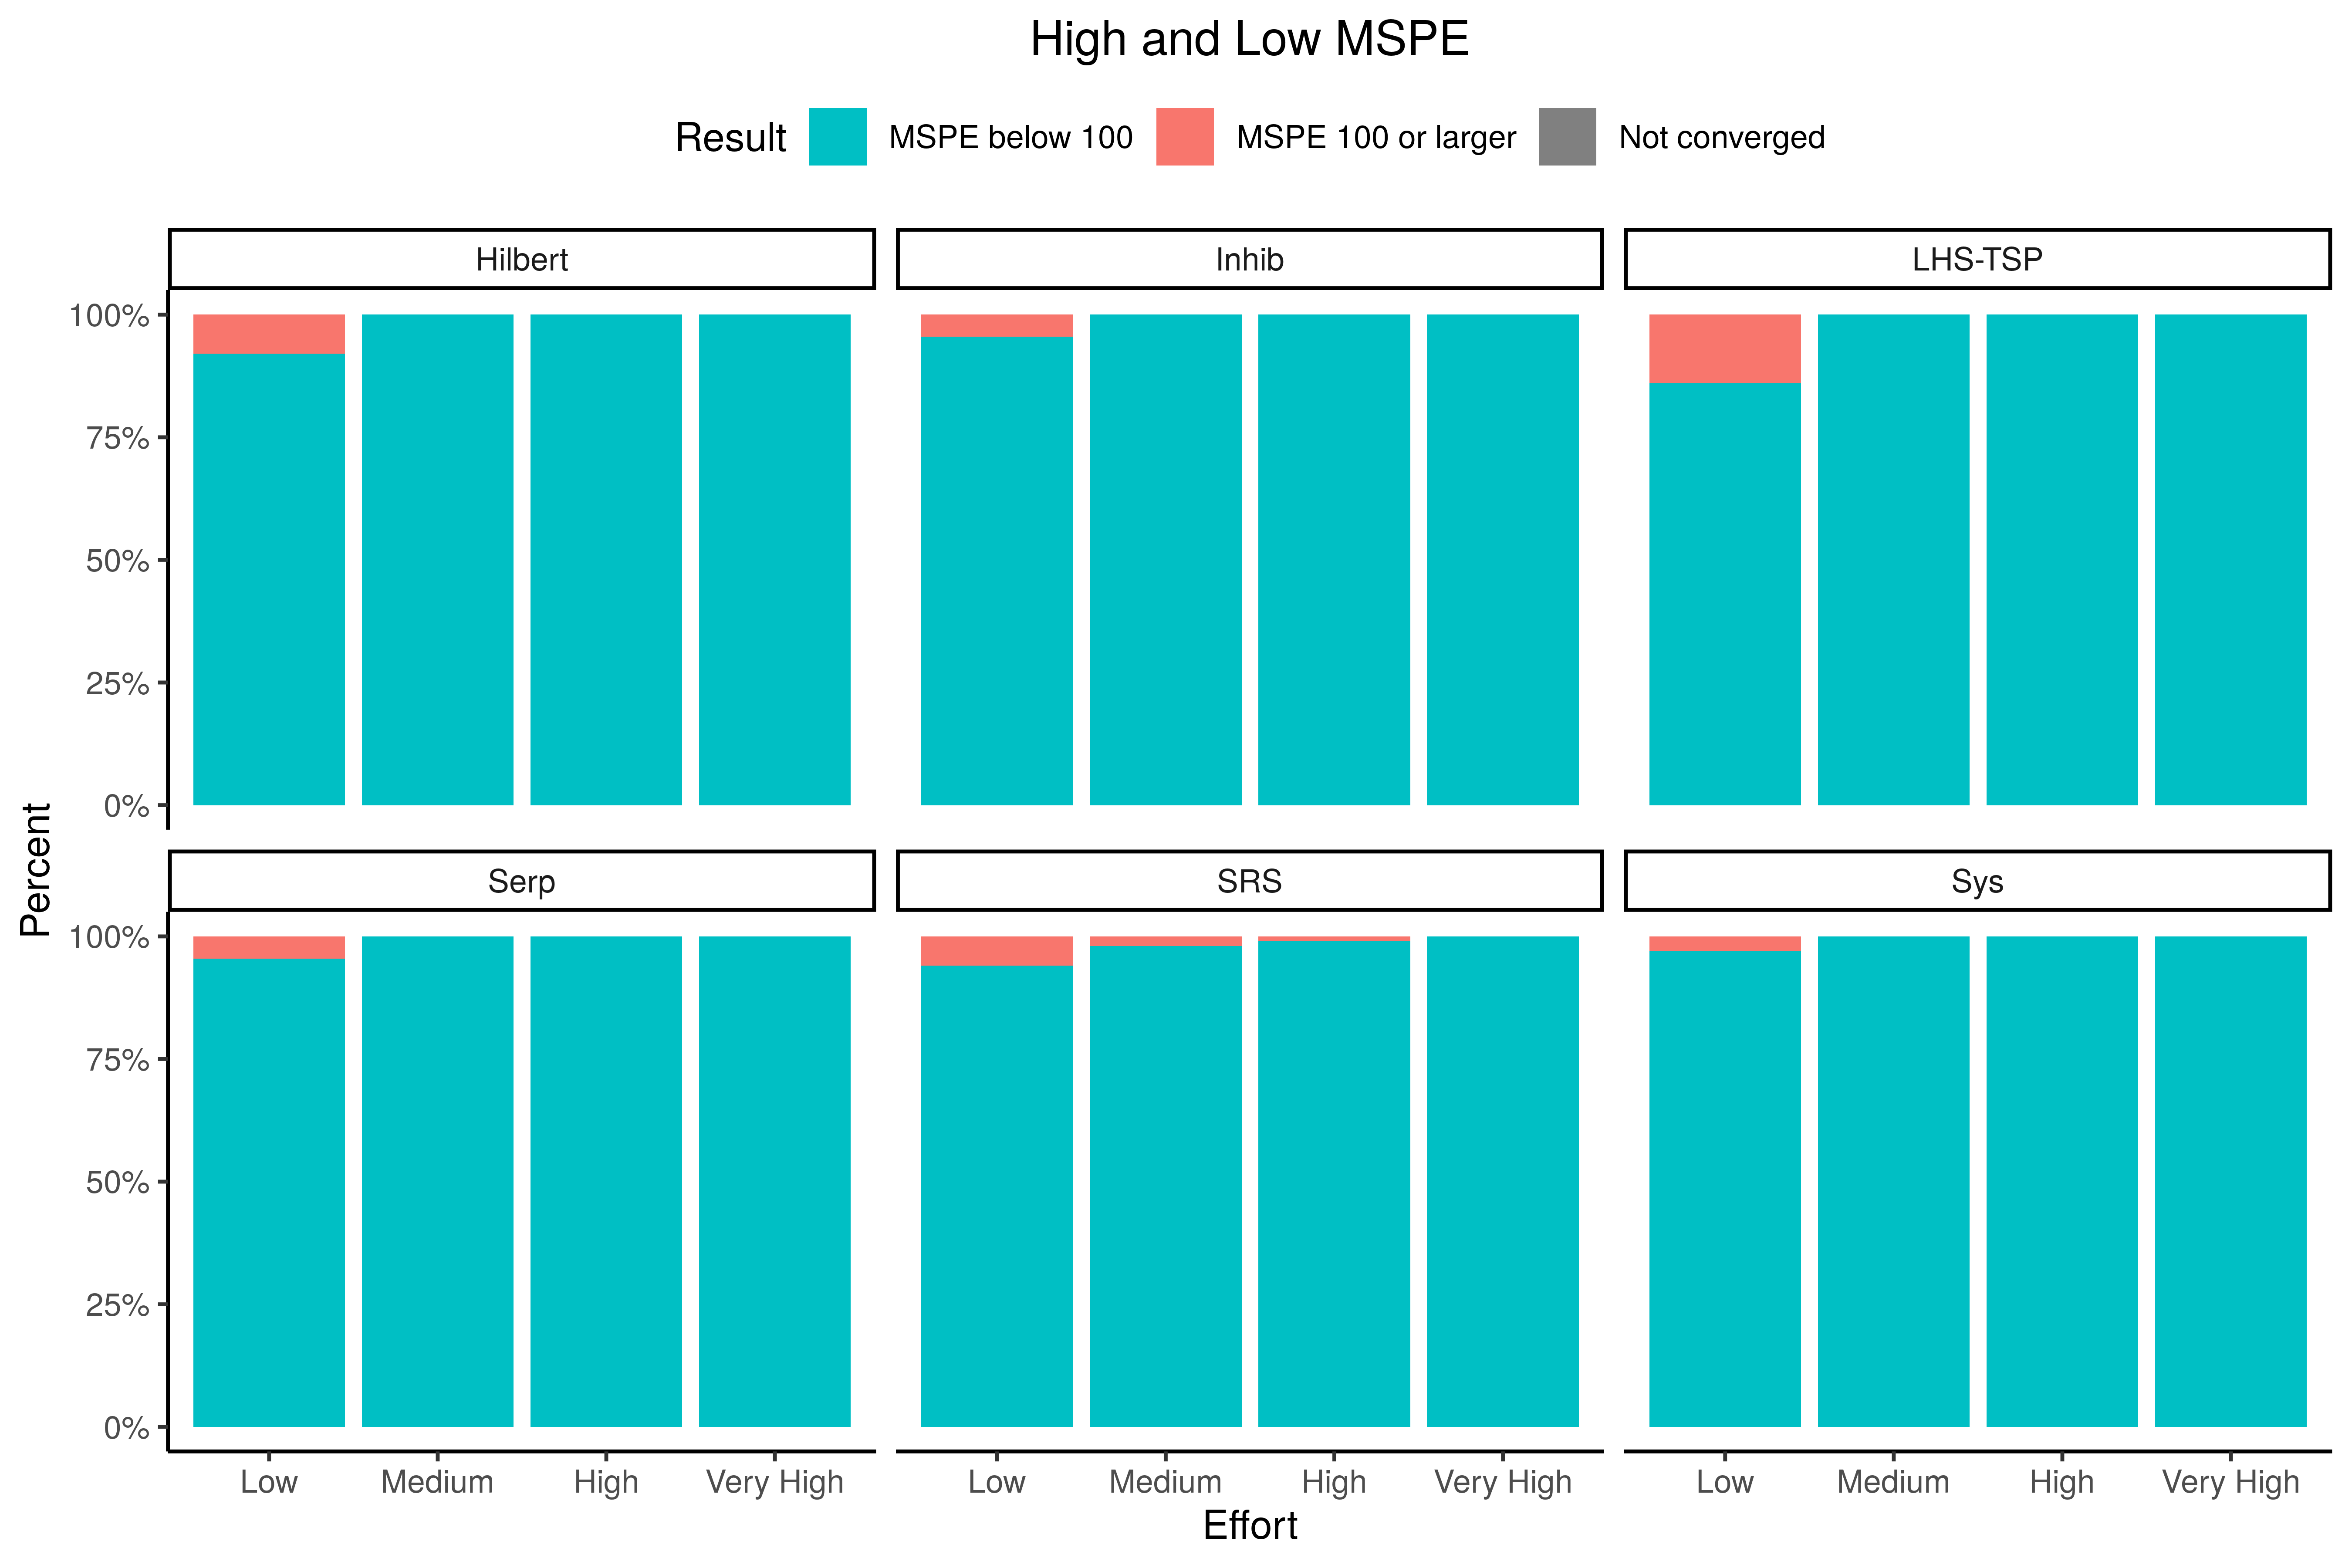
\includegraphics[width=4.5in]{../graphics/HighMSPE-Cluster000004.png}
\caption{MSPE distribution for one LGCP with Clusters dataset}
\label{highmspecluster}
\end{subfigure}

\caption{Plots of the distribution of high and low mean squared prediction
error (MSPE) vs survey effort for each plan applied to one realization of a
LGCP and one realization of a LGCP with Clusters.}
\label{histmsperesults}
\end{figure}


\subsection{Dealing with computational problems}
\label{compissues}

A notable proportion of simulation runs resulted in surfaces with edge effects
similar to Figure \ref{serp000148}, especially at lower levels of sampling
effort. This is most likely a symptom of the mesh not being able to represent
the posterior surface implied by the observed data. In practice, data analysts
should fit the model with several different meshes to assess adequacy of the
approximation.

We constructed a finer mesh with 1102 nodes (Figure \ref{meshfiner}), then
refit the model to the point pattern from Figure \ref{serp000148}. The
resulting log-intensity surface appears in Figure \ref{finer}. The surface is
free of edge effects or extreme values, has an MSPE of 2.31 (down from 1605),
and looks generally similar to well-performing surfaces from other simulation
runs using the same dataset (e.g. Figure \ref{srs000187lgcp}, more examples
in the Appendix~\ref{moreplots}).

This refined mesh has nearly four times as many nodes and the mesh used for
the full set of simulations, and consequently fitting the model takes several
times longer. The time requirement precluded us from rerunning the full
simulation study with this mesh, but the simulations using the coarse mesh
provide helpful insight into which schemes are more likely to require more
computation effort.

\begin{figure}
\includegraphics[width=5in]{../graphics/finermesh-LGCP000004.pdf}
\caption{Illustration of a finer mesh than the one used in the full simulation.
The mesh nodes are used in a numerical integration scheme where they are
weighted by the area of their dual cells (outlined in grey).}
\label{meshfiner}
\end{figure}

\begin{figure}

\begin{subfigure}{5in}
\includegraphics[width=5in]{../graphics/lambda-Finer-LGCP000004.pdf}
\caption{Predicted log-intensity}
\label{lambdafinerlgcp}
\end{subfigure}

\begin{subfigure}{5in}
\includegraphics[width=5in]{../graphics/lambdaSD-Finer-LGCP000004.pdf}
\caption{Prediction SD}
\label{sdfinerlgcp}
\end{subfigure}

\caption{Predicted GP surface and prediction SD using data observed via a
serpentine transect plan. When these data are modeled with a coarser mesh, the
prediction surface exhibits numerical instability. This refined mesh results in
a much-improved prediction surface.}
\label{finer}
\end{figure}


\subsection{LGCP simulation results}

Considered across all survey plans applied to one LGCP dataset, most
95\% posterior intervals capture the true mean value, but those that did not
were more likely to underestimate than overestimate the mean (Figure
\ref{intlgcp}). The capture rate increases with survey effort, with only
the SRS and Hilbert schemes being observed to miss the true mean at the
highest effort level.
%For each scheme at each effort level, the median
%error in the posterior mean was between 0 and \(-1\). At any given effort
%level, there is little difference among the distribution of errors across
%schemes. However, at low and medium effort, all of these distributions
%have long right tails with severe overestimates (accompanied by wide
%posterior intervals).

Both MSPE and APV had right-skewed distributions. Thus we use logarithmic
scales for plots and summarize them using the median and interquartile range
(IQR). Median MSPE decreases with increasing path distance, leveling off
between the medium and high effort levels (Figure~\ref{mspelgcp}). Variability
(IQR) of MSPE also decreases as effort increases. Prediction surfaces with edge
effects form a cluster of large, outlying MSPE values. At all levels of effort,
systematic designs had the least variability in MSPE. The lowest-MSPE
prediction surfaces result from the longest Hilbert designs, but the
distributions of MSPE are similar for all schemes at the high and very effort
levels. Overall, the differences among the different schemes with respect to
median MSPE are much less than the variability in MSPE within each effort
level. The results are largely the same for APV (Figure \ref{apvlgcp}).
% More specifically, this last sentence means there was "more" variation across
% realizations than with variations. No scheme was best or least variable for
% all realizations.

%The relationship between APV and MSPE differs from realization to realization
%(Figure~\ref{apvresults}). Surfaces in the high-MSPE cluster have high APV, but
%otherwise there is little association between APV and MSPE.
% Point out which did best anyways.

%\emph{Maybe omit fits with \(\mathrm{MSPE} > 100\) from other results?}

%\begin{itemize}
%\item LHS-TSP has lowest median APV for paths under 10000 units but large IQR
%\item For longer paths, SRS isn't bad
%\item SRS has slightly lower median and IQR of APV than systematic
%\item The longest serp designs with 5 zigzags have lowest IQR of MSPE and APV
%\item Inhib has high variability for clustered data
%\item Lowest MSPE designs were Hilbert order 6
%\end{itemize}

\begin{figure}

\begin{subfigure}{4.5in}
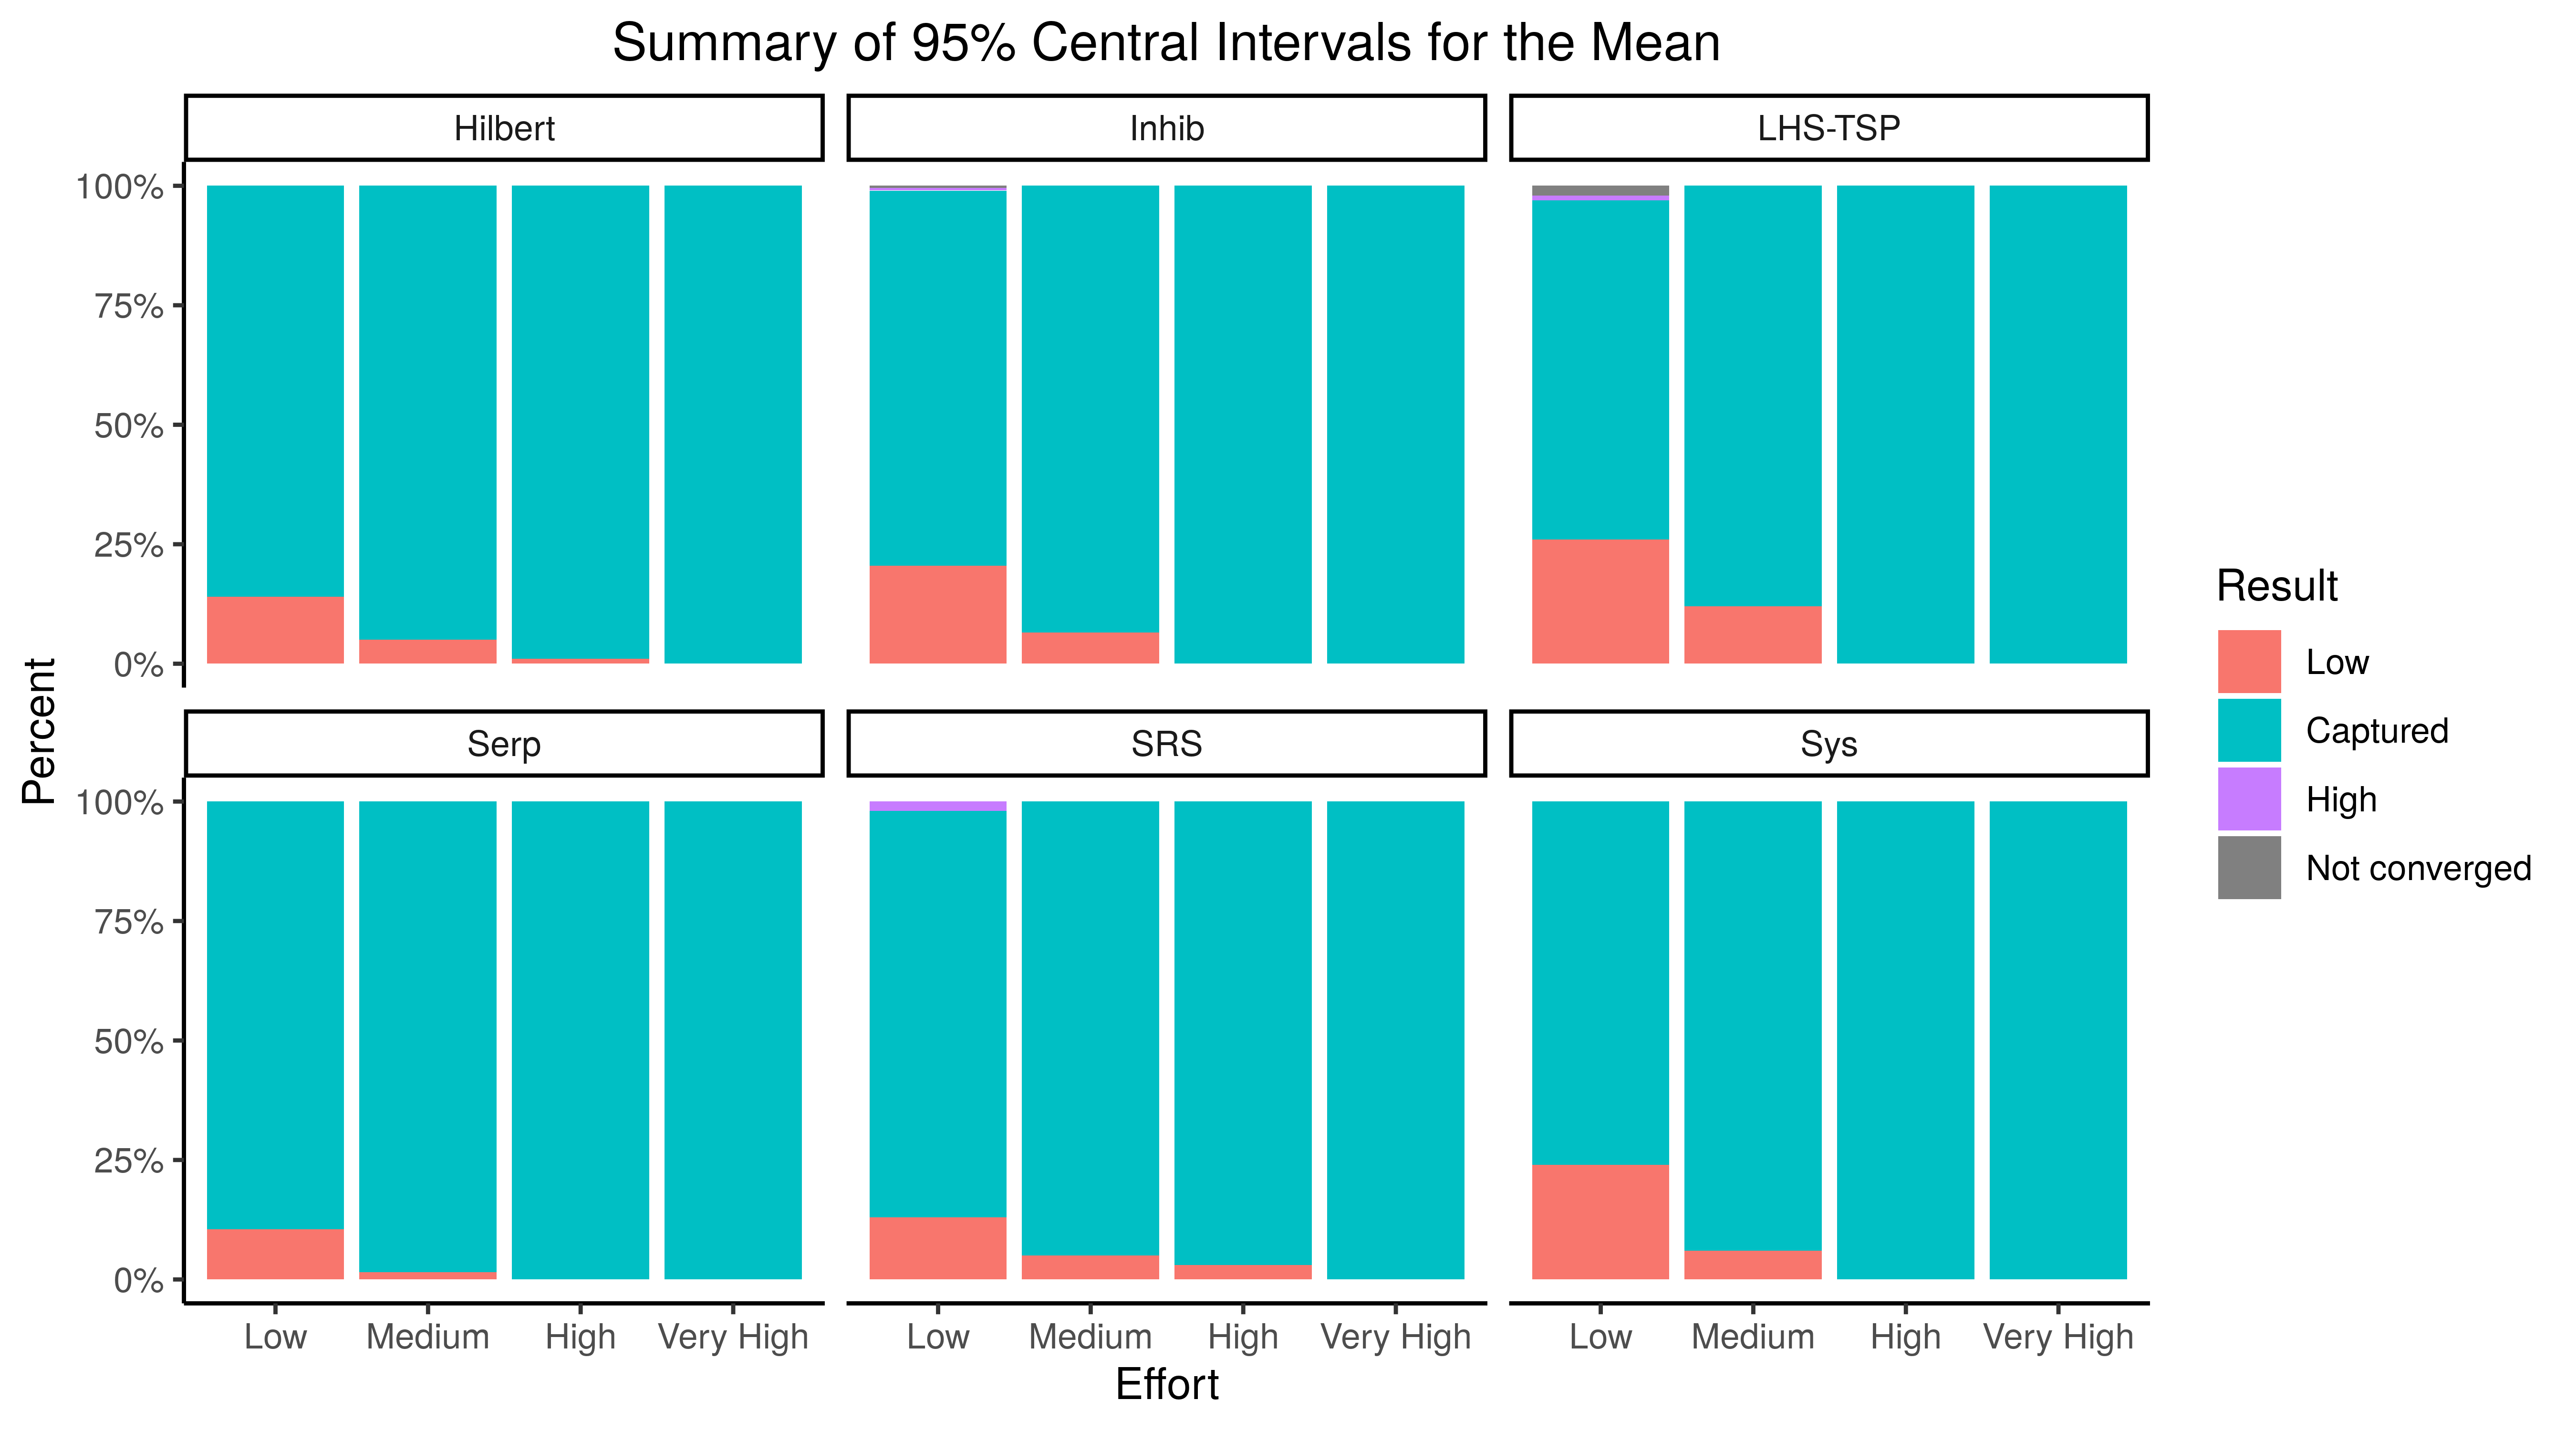
\includegraphics[width=4.5in]{../graphics/IntCapture-LGCP000004.png}
\caption{Comparisons of posterior intervals for the intercept to the true mean
for one LGCP dataset}
\label{intlgcp}
\end{subfigure}

\begin{subfigure}{4.5in}
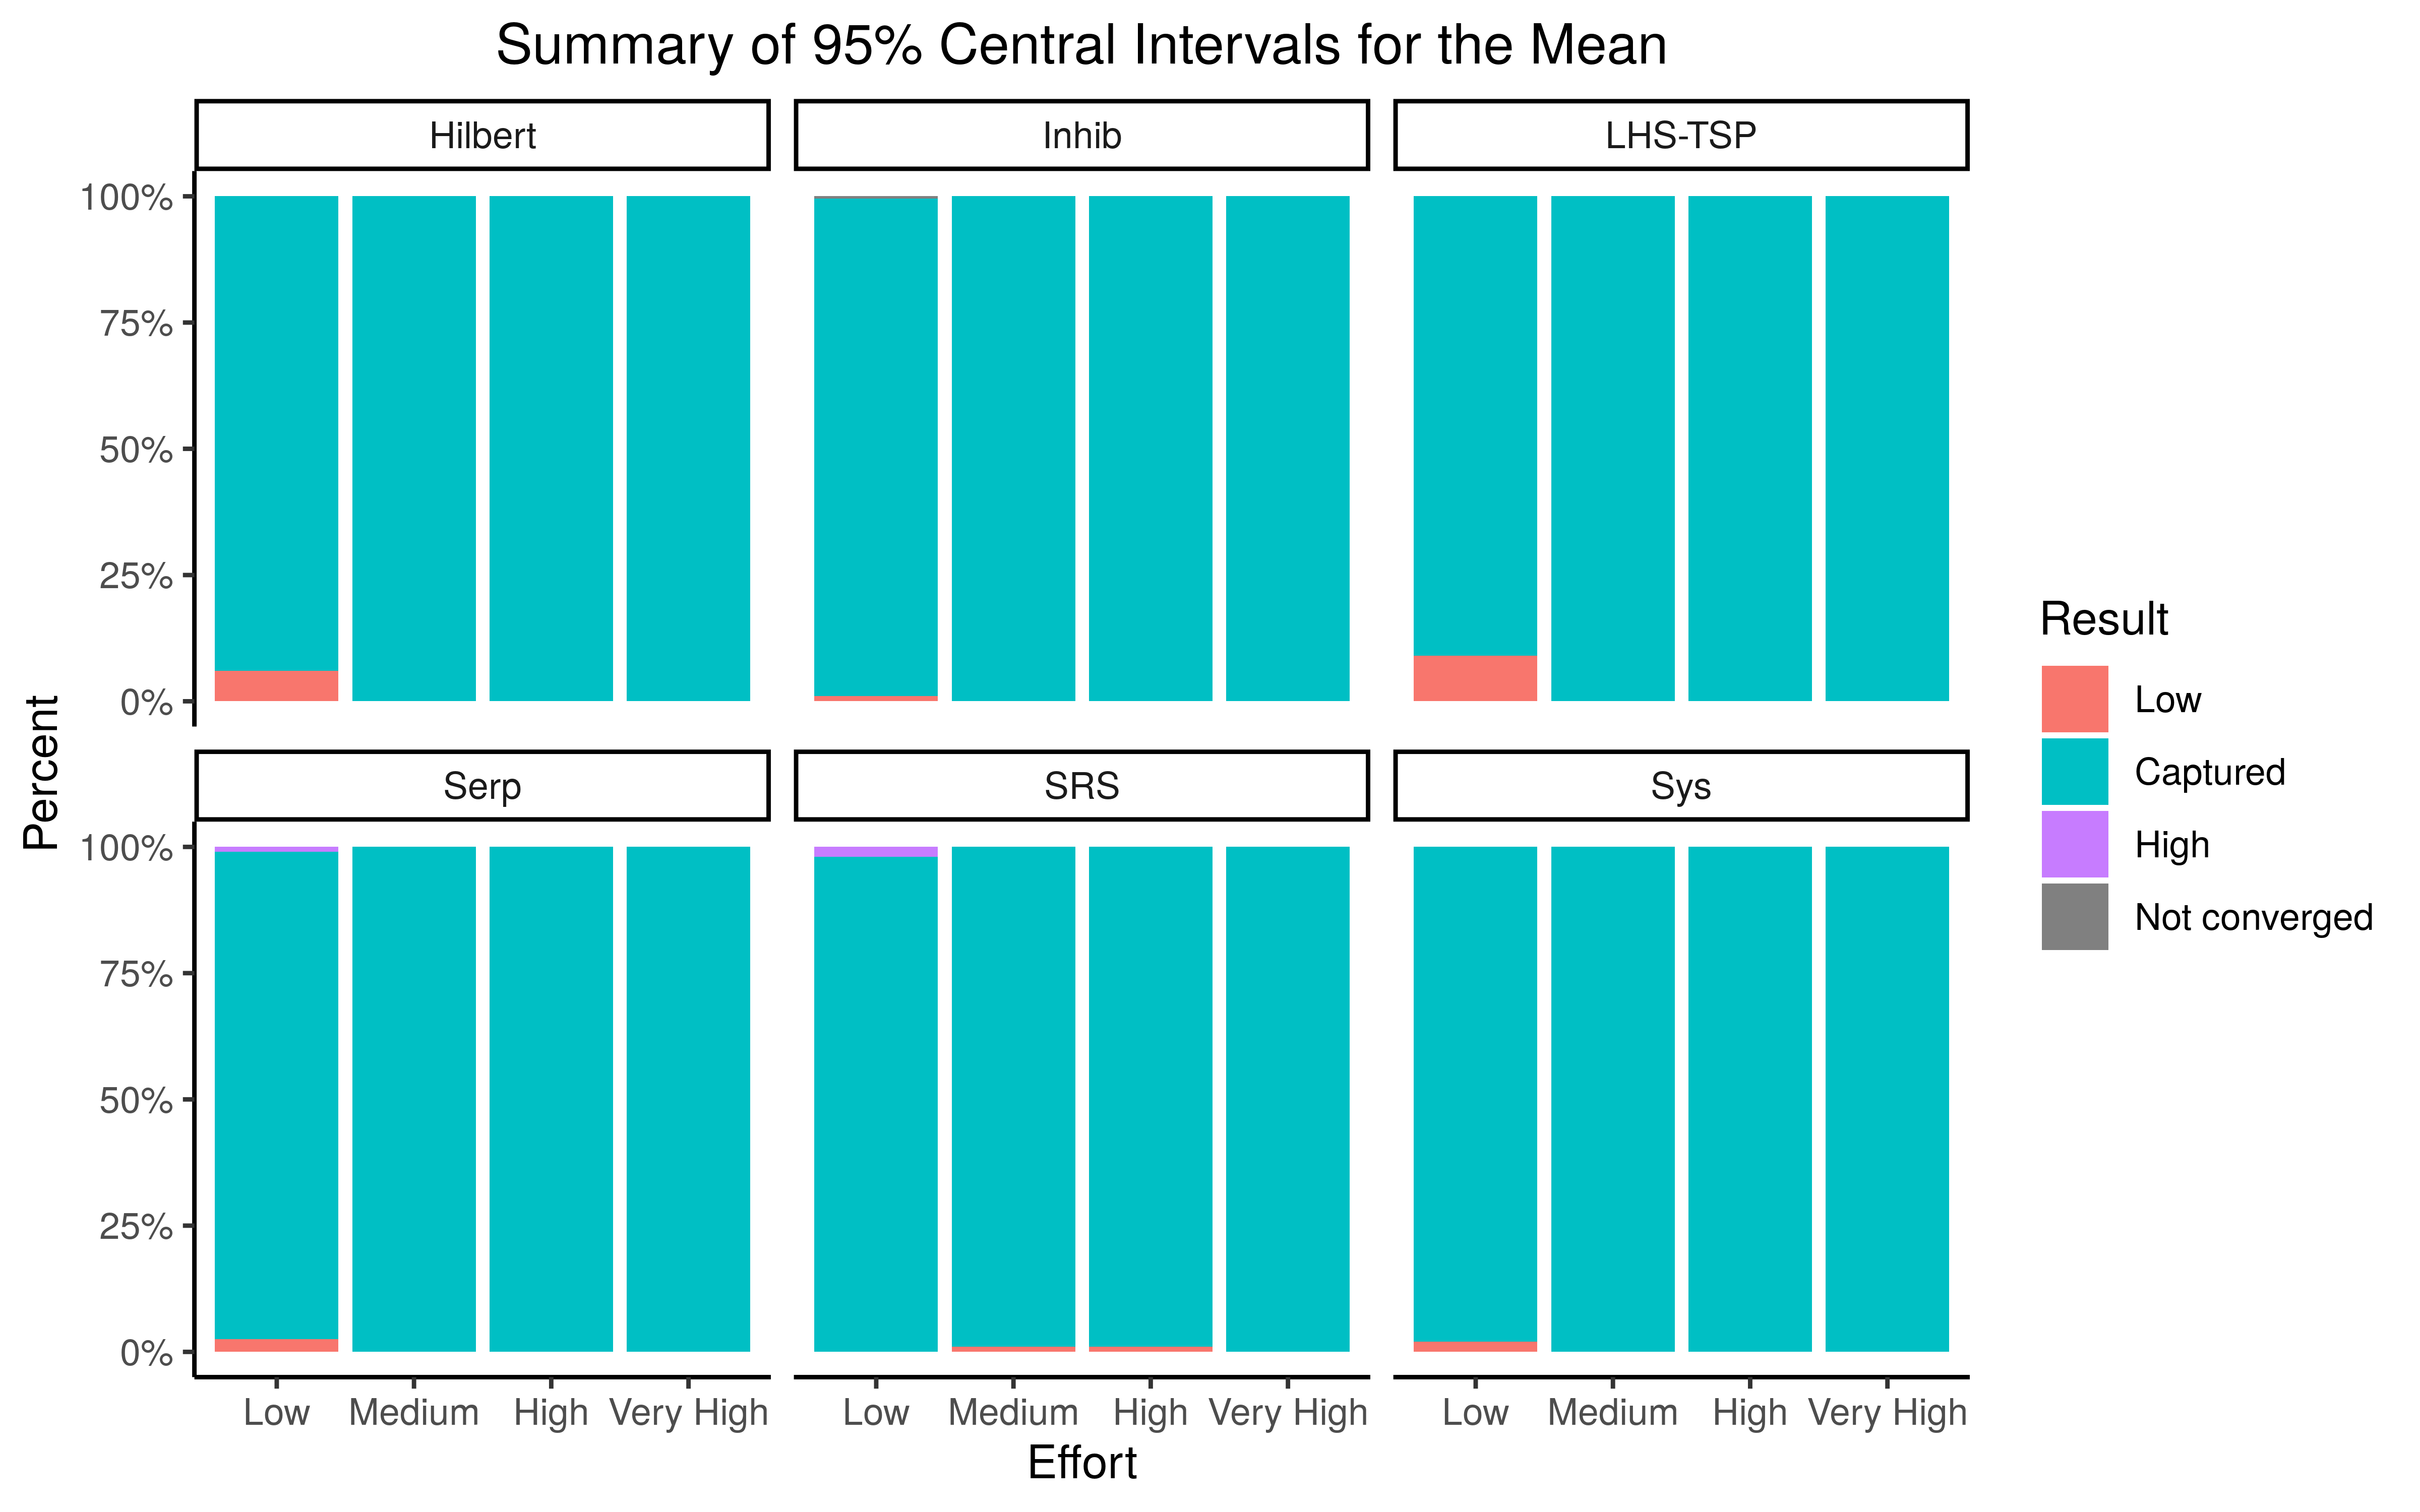
\includegraphics[width=4.5in]{../graphics/IntCapture-Cluster000004.png}
\caption{Comparisons of posterior intervals for the intercept to the true mean
for one LGCP with Clusters dataset}
\label{intclust}
\end{subfigure}

\caption{Plots summarizing comparisons between central 95\% posterior intervals
for the intercept and the true mean log-intensity of the realized GP.
``Captured'' indicates that the true mean is inside the interval. ``High'' and
``Low'' indicate that the entire interval is, respectively, above or below the
true mean.}
\label{intresults}
\end{figure}

\begin{figure}

\begin{subfigure}{4.5in}
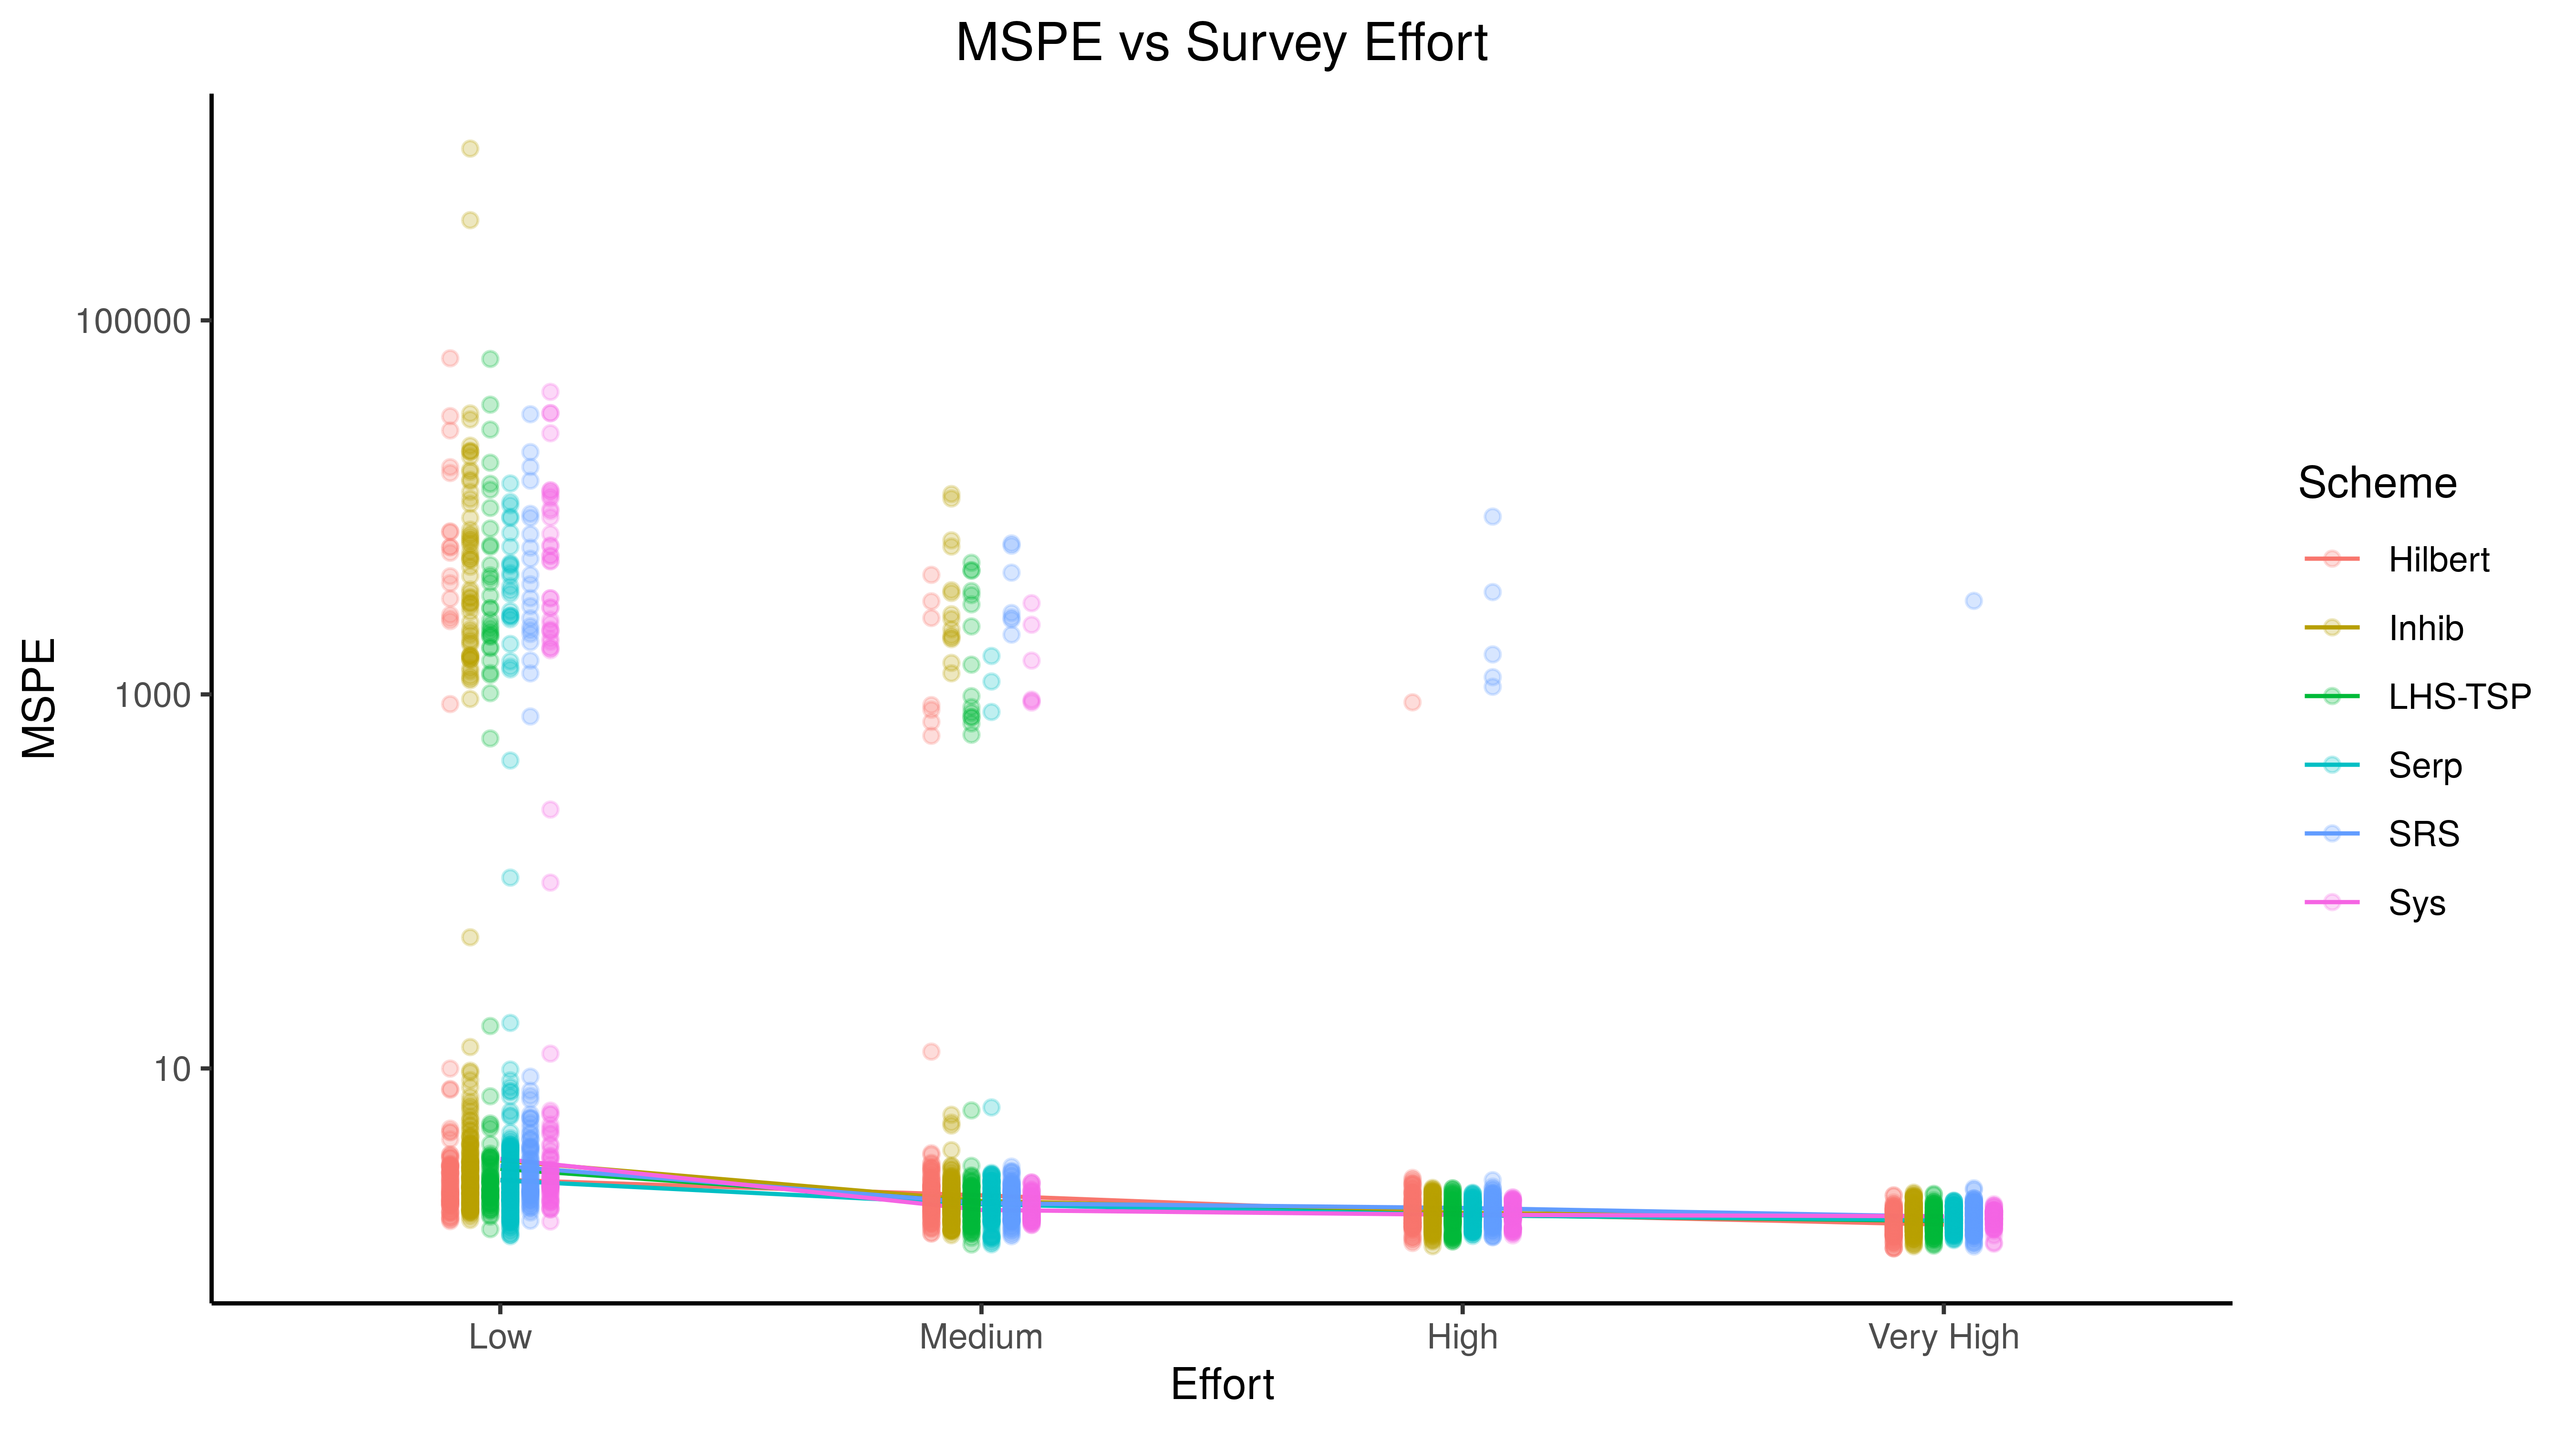
\includegraphics[width=4.5in]{../graphics/MSPE-effort-notpaneled-LGCP000004.png}
\caption{MSPE vs survey effort for one LGCP dataset}
\label{mspelgcp}
\end{subfigure}

\begin{subfigure}{4.5in}
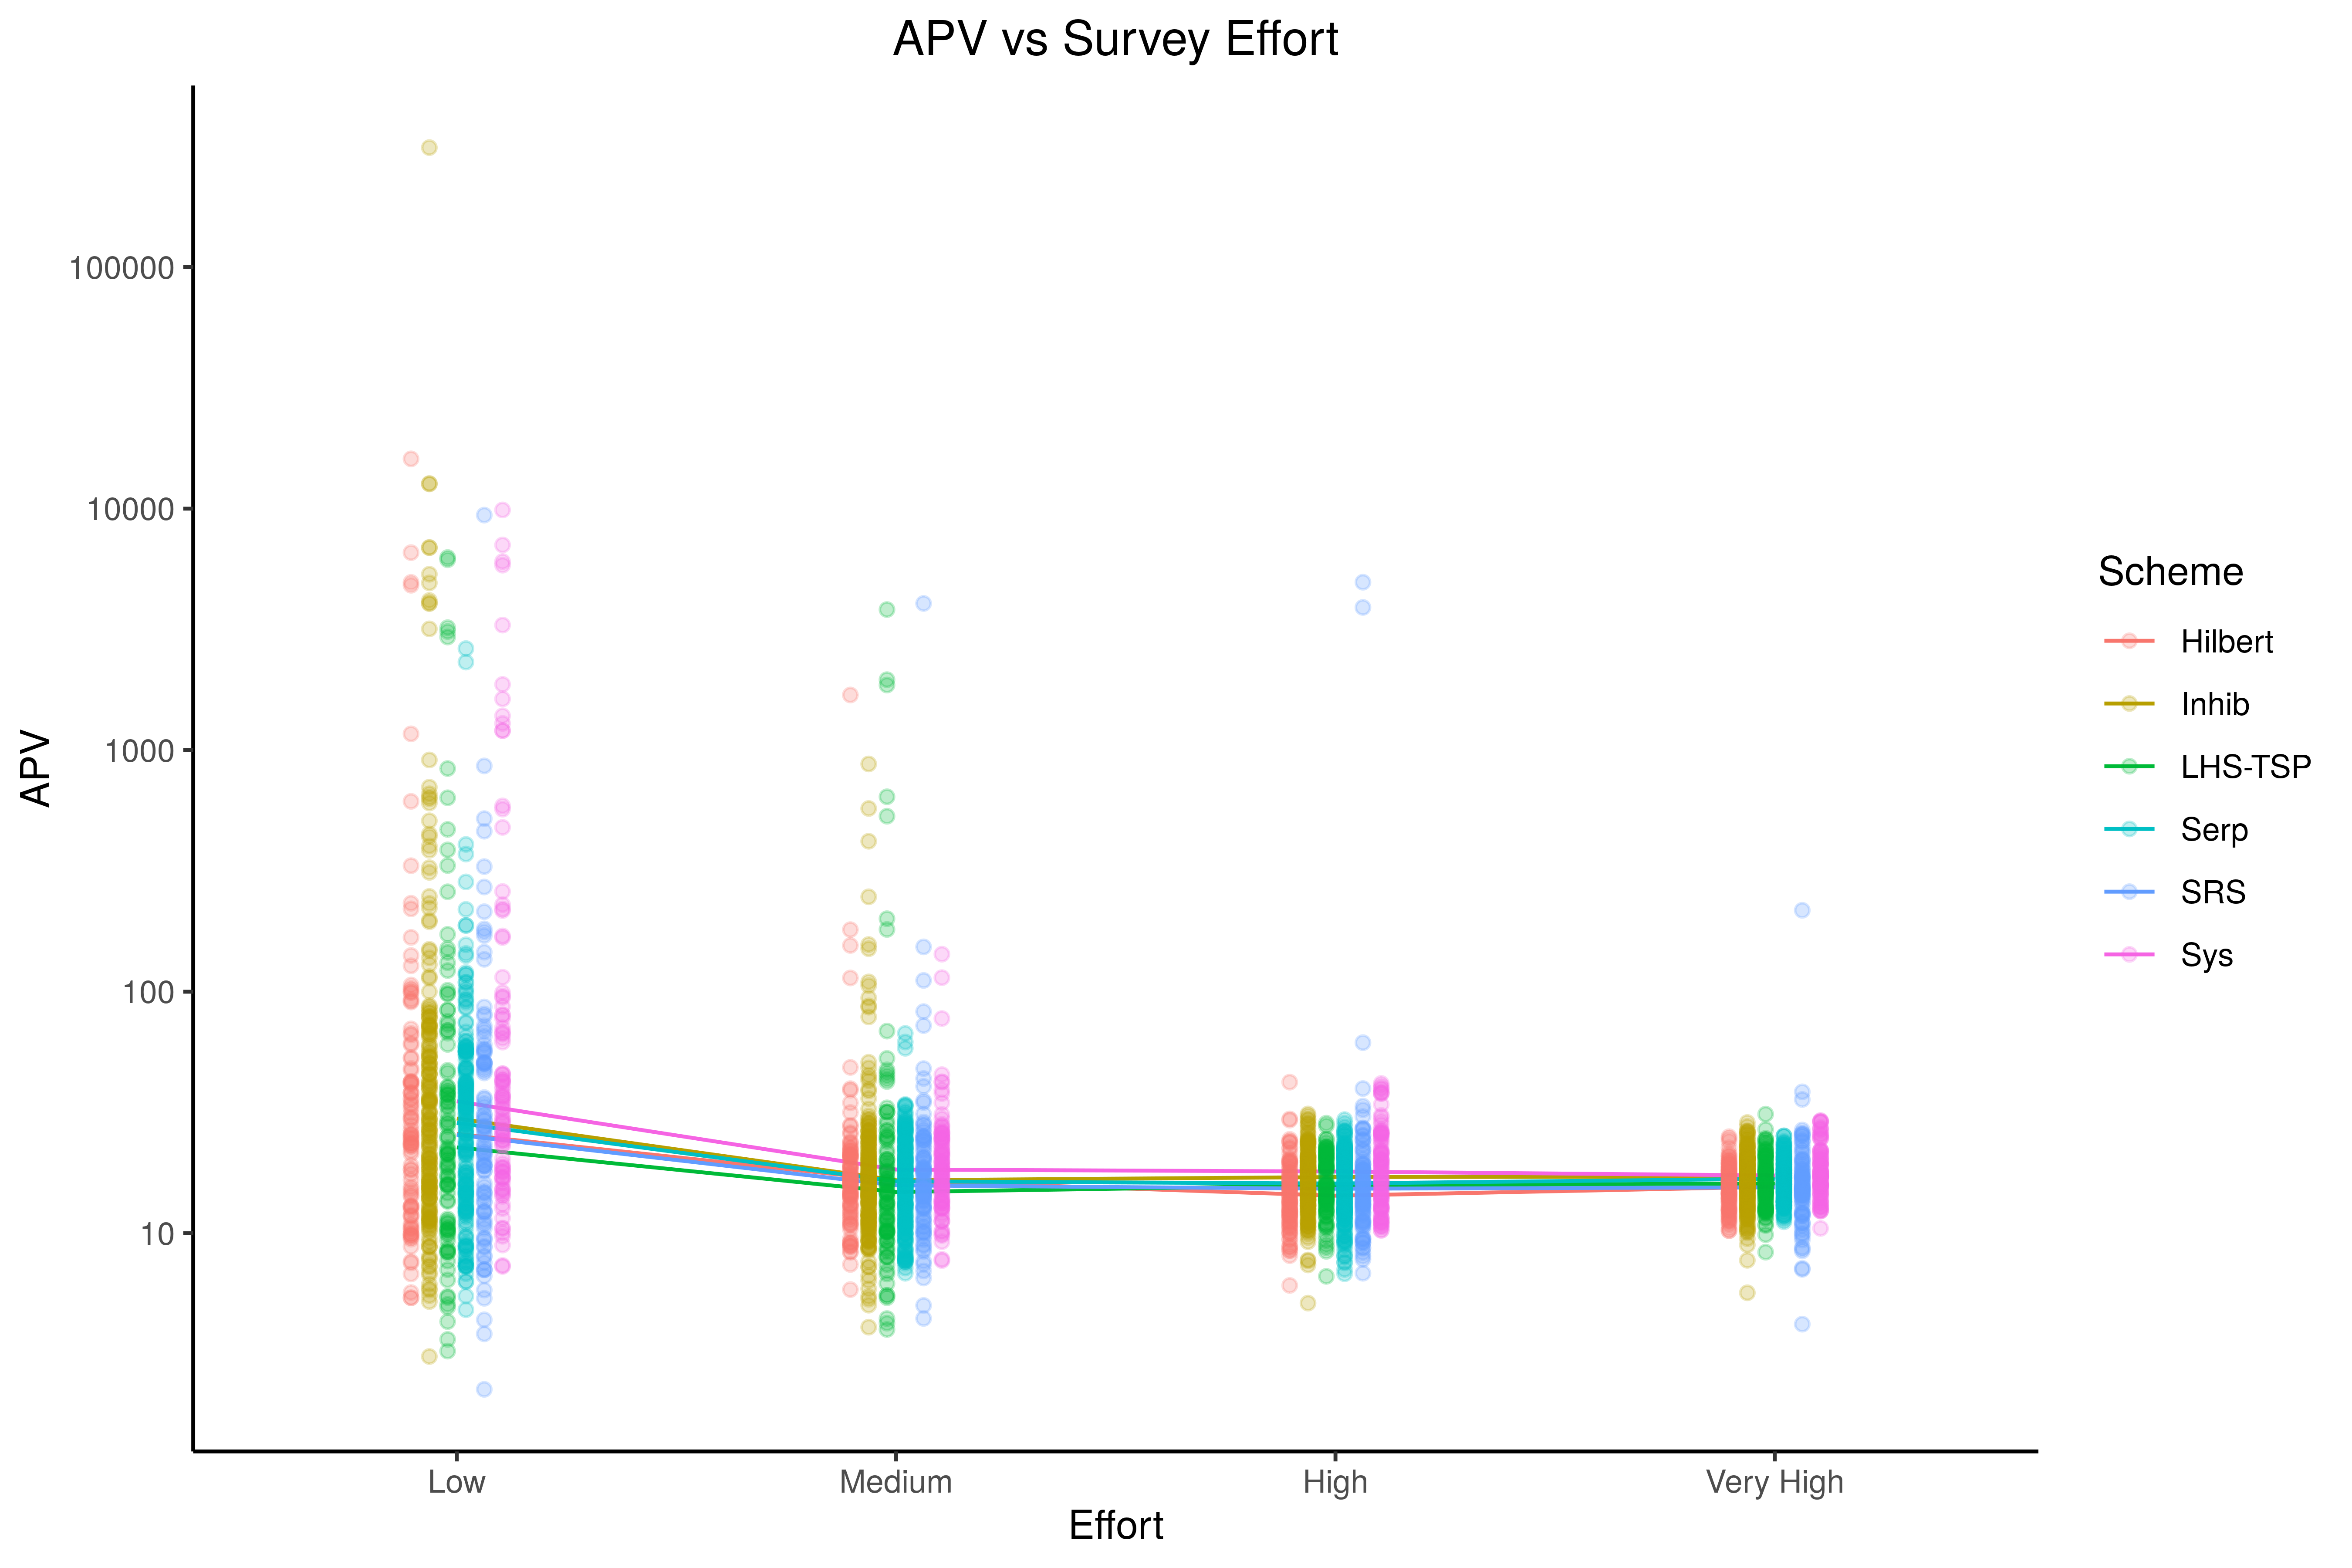
\includegraphics[width=4.5in]{../graphics/APV-effort-notpaneled-LGCP000004.png}
\caption{APV vs survey effort for one LGCP dataset}
\label{apvlgcp}
\end{subfigure}

\caption{Plots of mean squared prediction error (MSPE) and average prediction
variance (APV) vs survey effort for each plan applied to one realization of a
LGCP. Line segments connect the median at each effort level.}
\label{lgcpresults}
\end{figure}

%\begin{figure}
%
%\begin{subfigure}{4.5in}
%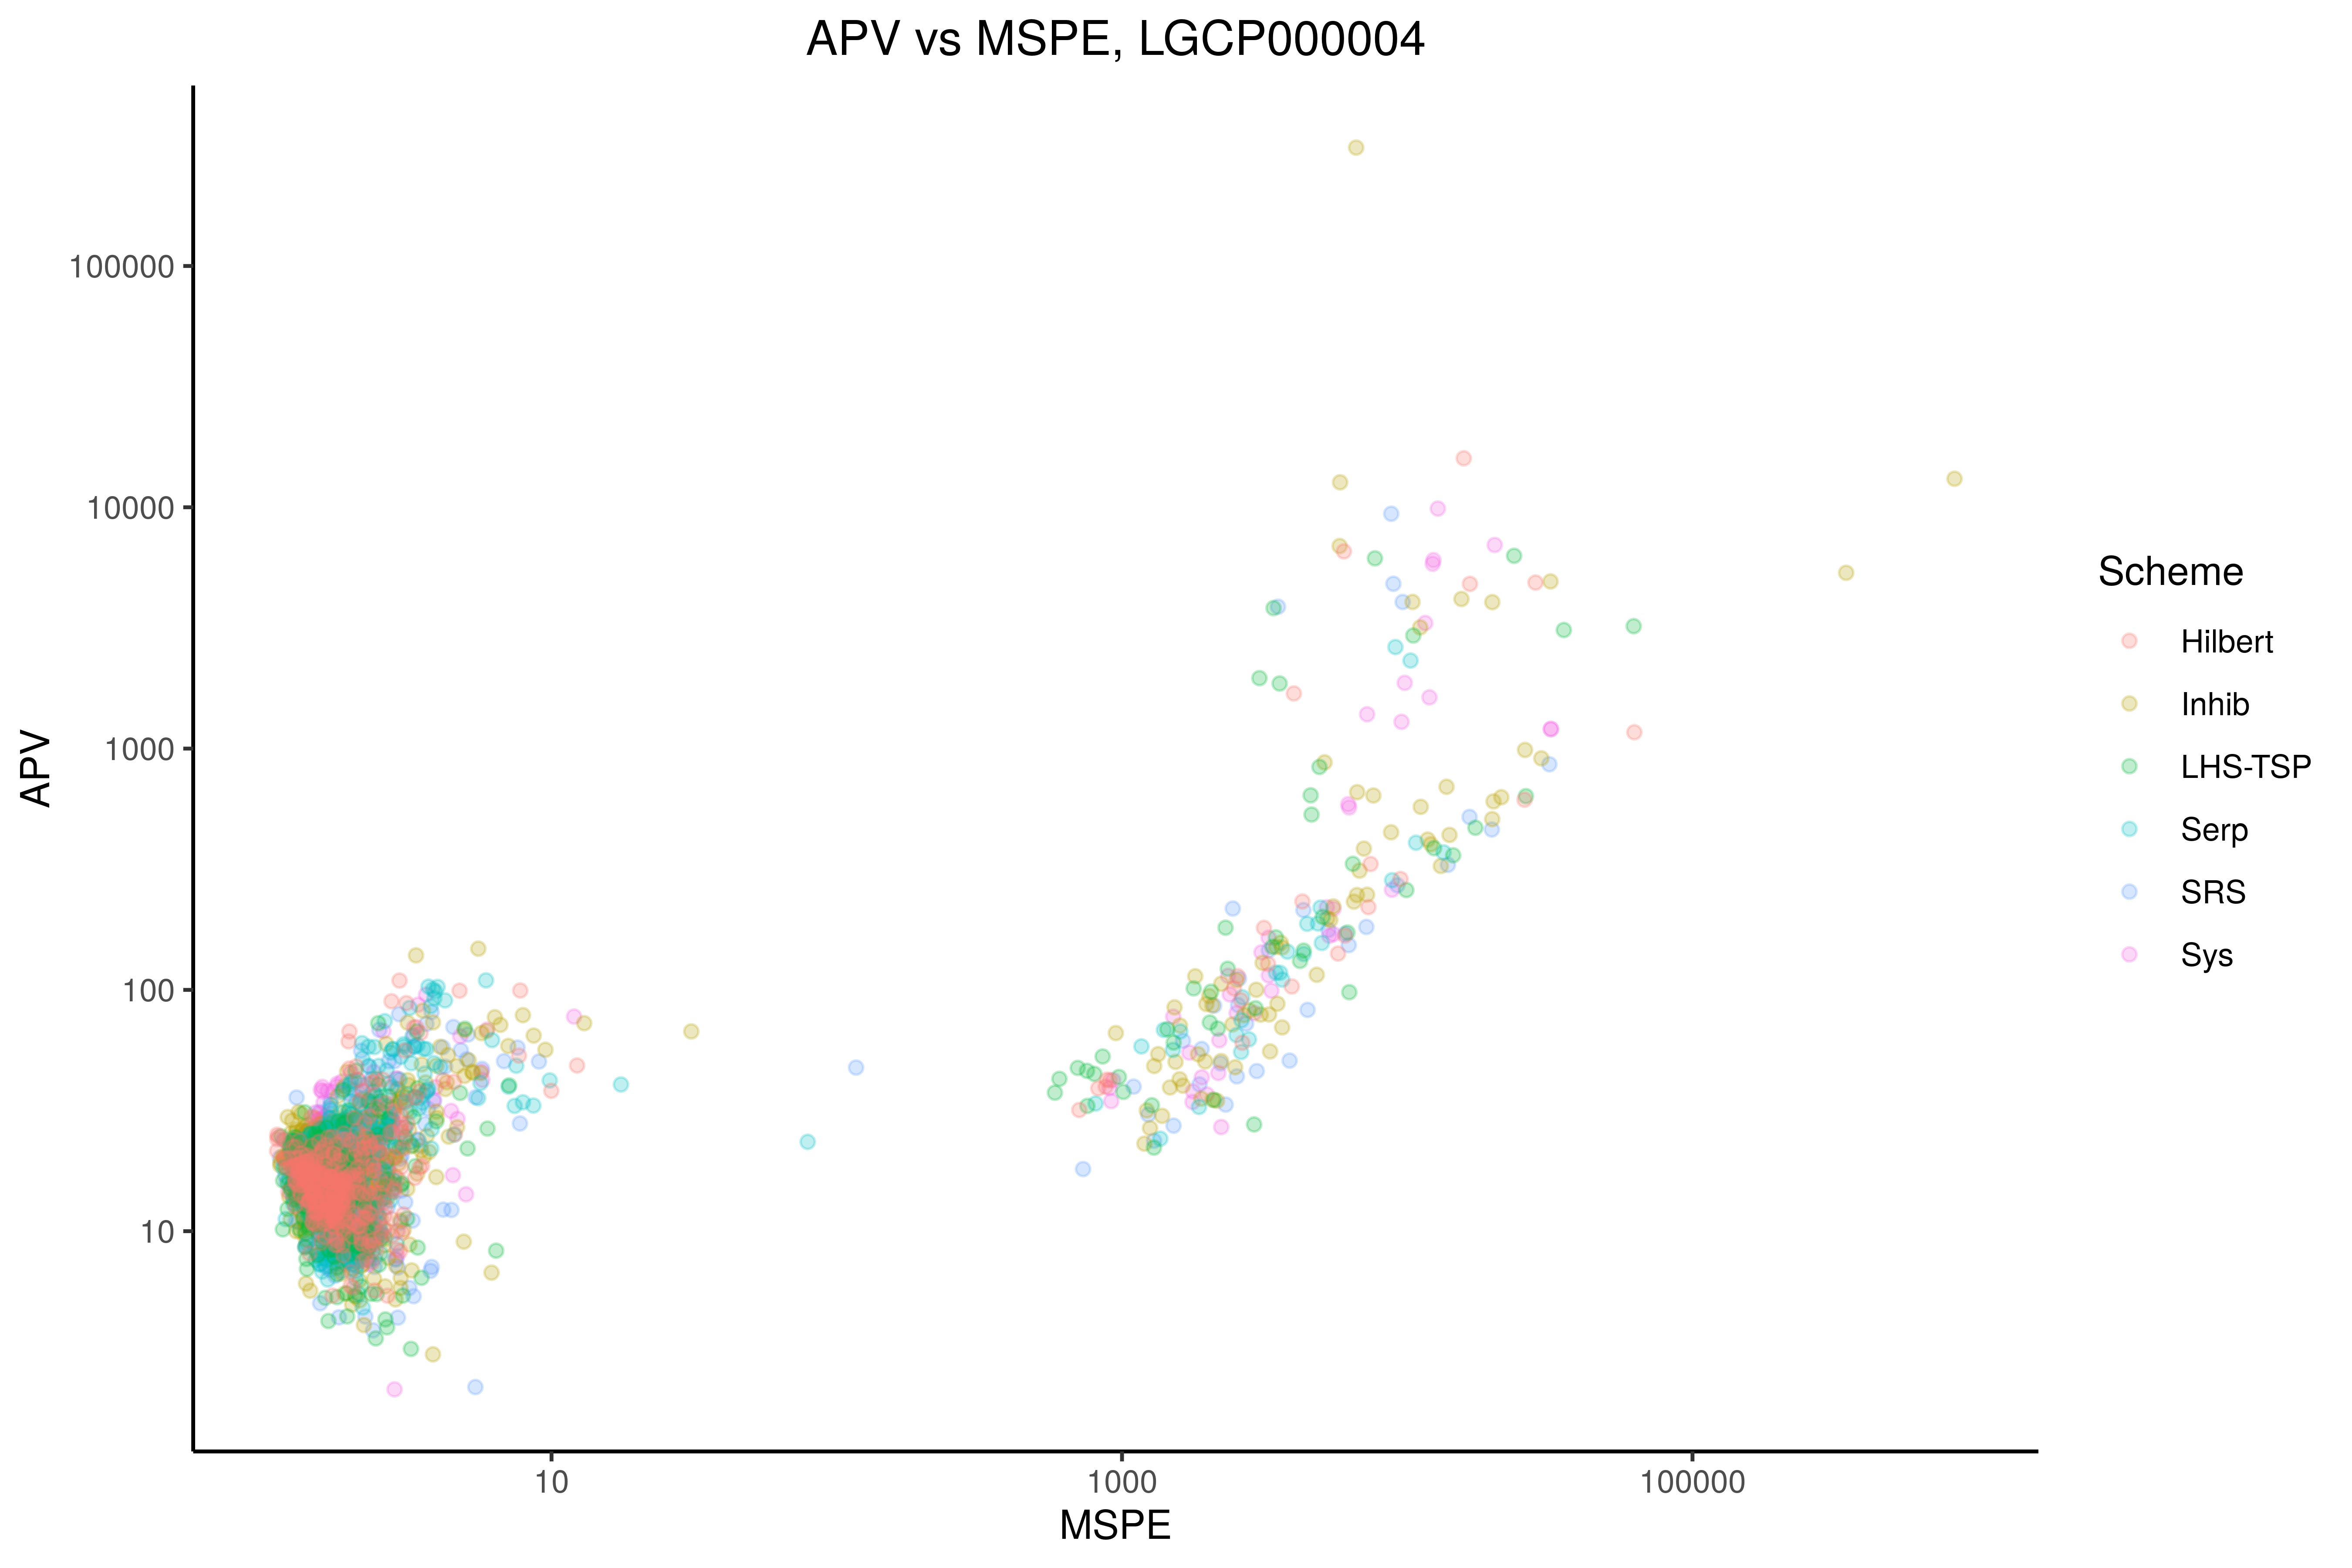
\includegraphics[width=4.5in]{../graphics/APV-MSPE-LGCP000004.png}
%\caption{APV vs MSPE for one LGCP dataset}
%\label{apvlgcp}
%\end{subfigure}
%
%\begin{subfigure}{4.5in}
%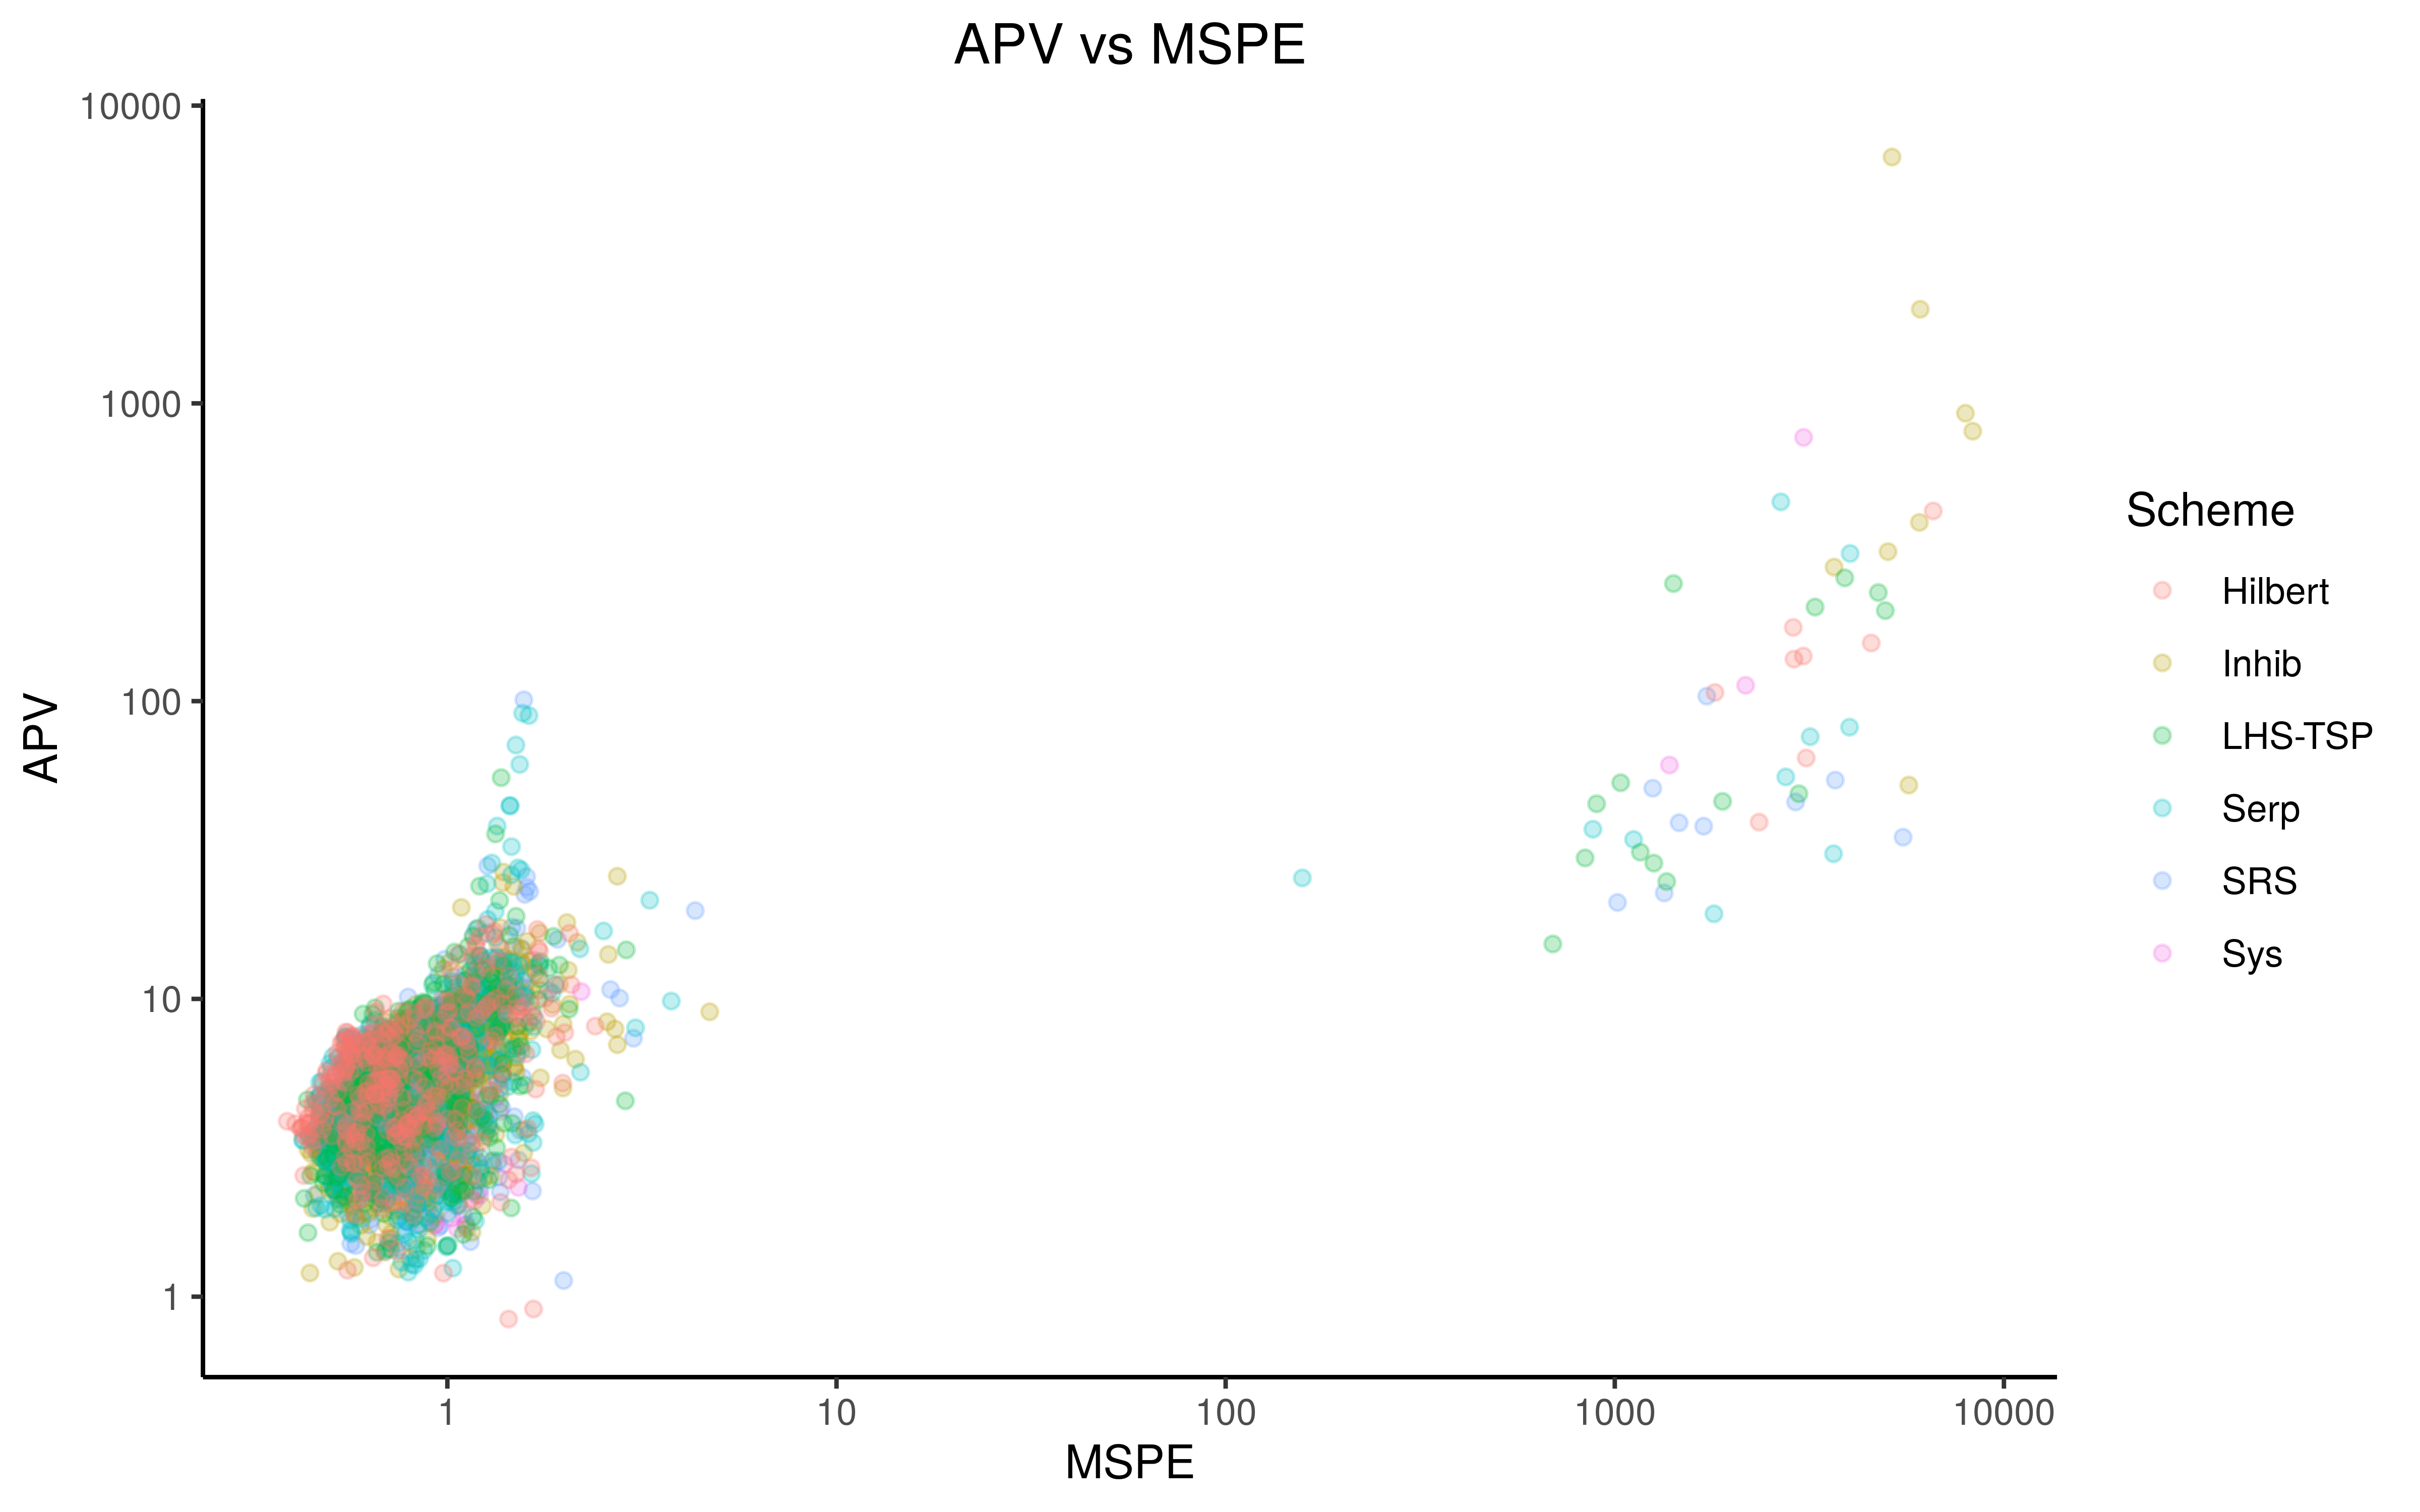
\includegraphics[width=4.5in]{../graphics/APV-MSPE-Cluster000004.png}
%\caption{APV vs MSPE for one LGCP with Clusters dataset}
%\label{apvcluster}
%\end{subfigure}
%
%\caption{Plots of average prediction variance (APV) vs MSPE for each plan
%applied to one realization of a LGCP and one realization of a LGCP with a
%Clusters.}
%\label{apvresults}
%\end{figure}


\subsection{LGCP with Clusters simulation results}

For the LGCP with Clusters dataset, all schemes tended to do well at
estimating the mean (Figure \ref{intclust}). At low effort, all schemes
occasionally fail to capture the true mean in a 95\% central posterior
interval. Only the SRS scheme is observed to miss the mean at medium or high
effort.
%The median errors for the scheme and effort combinations range
%between \(-0.13\) and 0.16. IQR decreases slightly with higher effort. At low
%effort, all schemes have long-tailed distributions containing some extreme
%errors; notably the serpentine and SRS schemes have left-tailed distributions
%while the others are right-tailed.

MSPE and APV again had right-skewed distributions. Median MSPE decreases as
effort increases (Figure~\ref{mspeclust}). Variability in MSPE is roughly
constant across effort levels. The systematic scheme had the lowest median
MSPE for low and medium effort and low IQR for all effort levels, while the
serpentine and Hilbert schemes have the lowest median at high and very high
effort. However, differences between schemes are much less than differences
across survey effort. At low effort, the distribution of APV has a long tail.
Otherwise there is little difference in distribution of APV across schemes or
effort (Figure \ref{apvclust}).

\begin{figure}

\begin{subfigure}{4.5in}
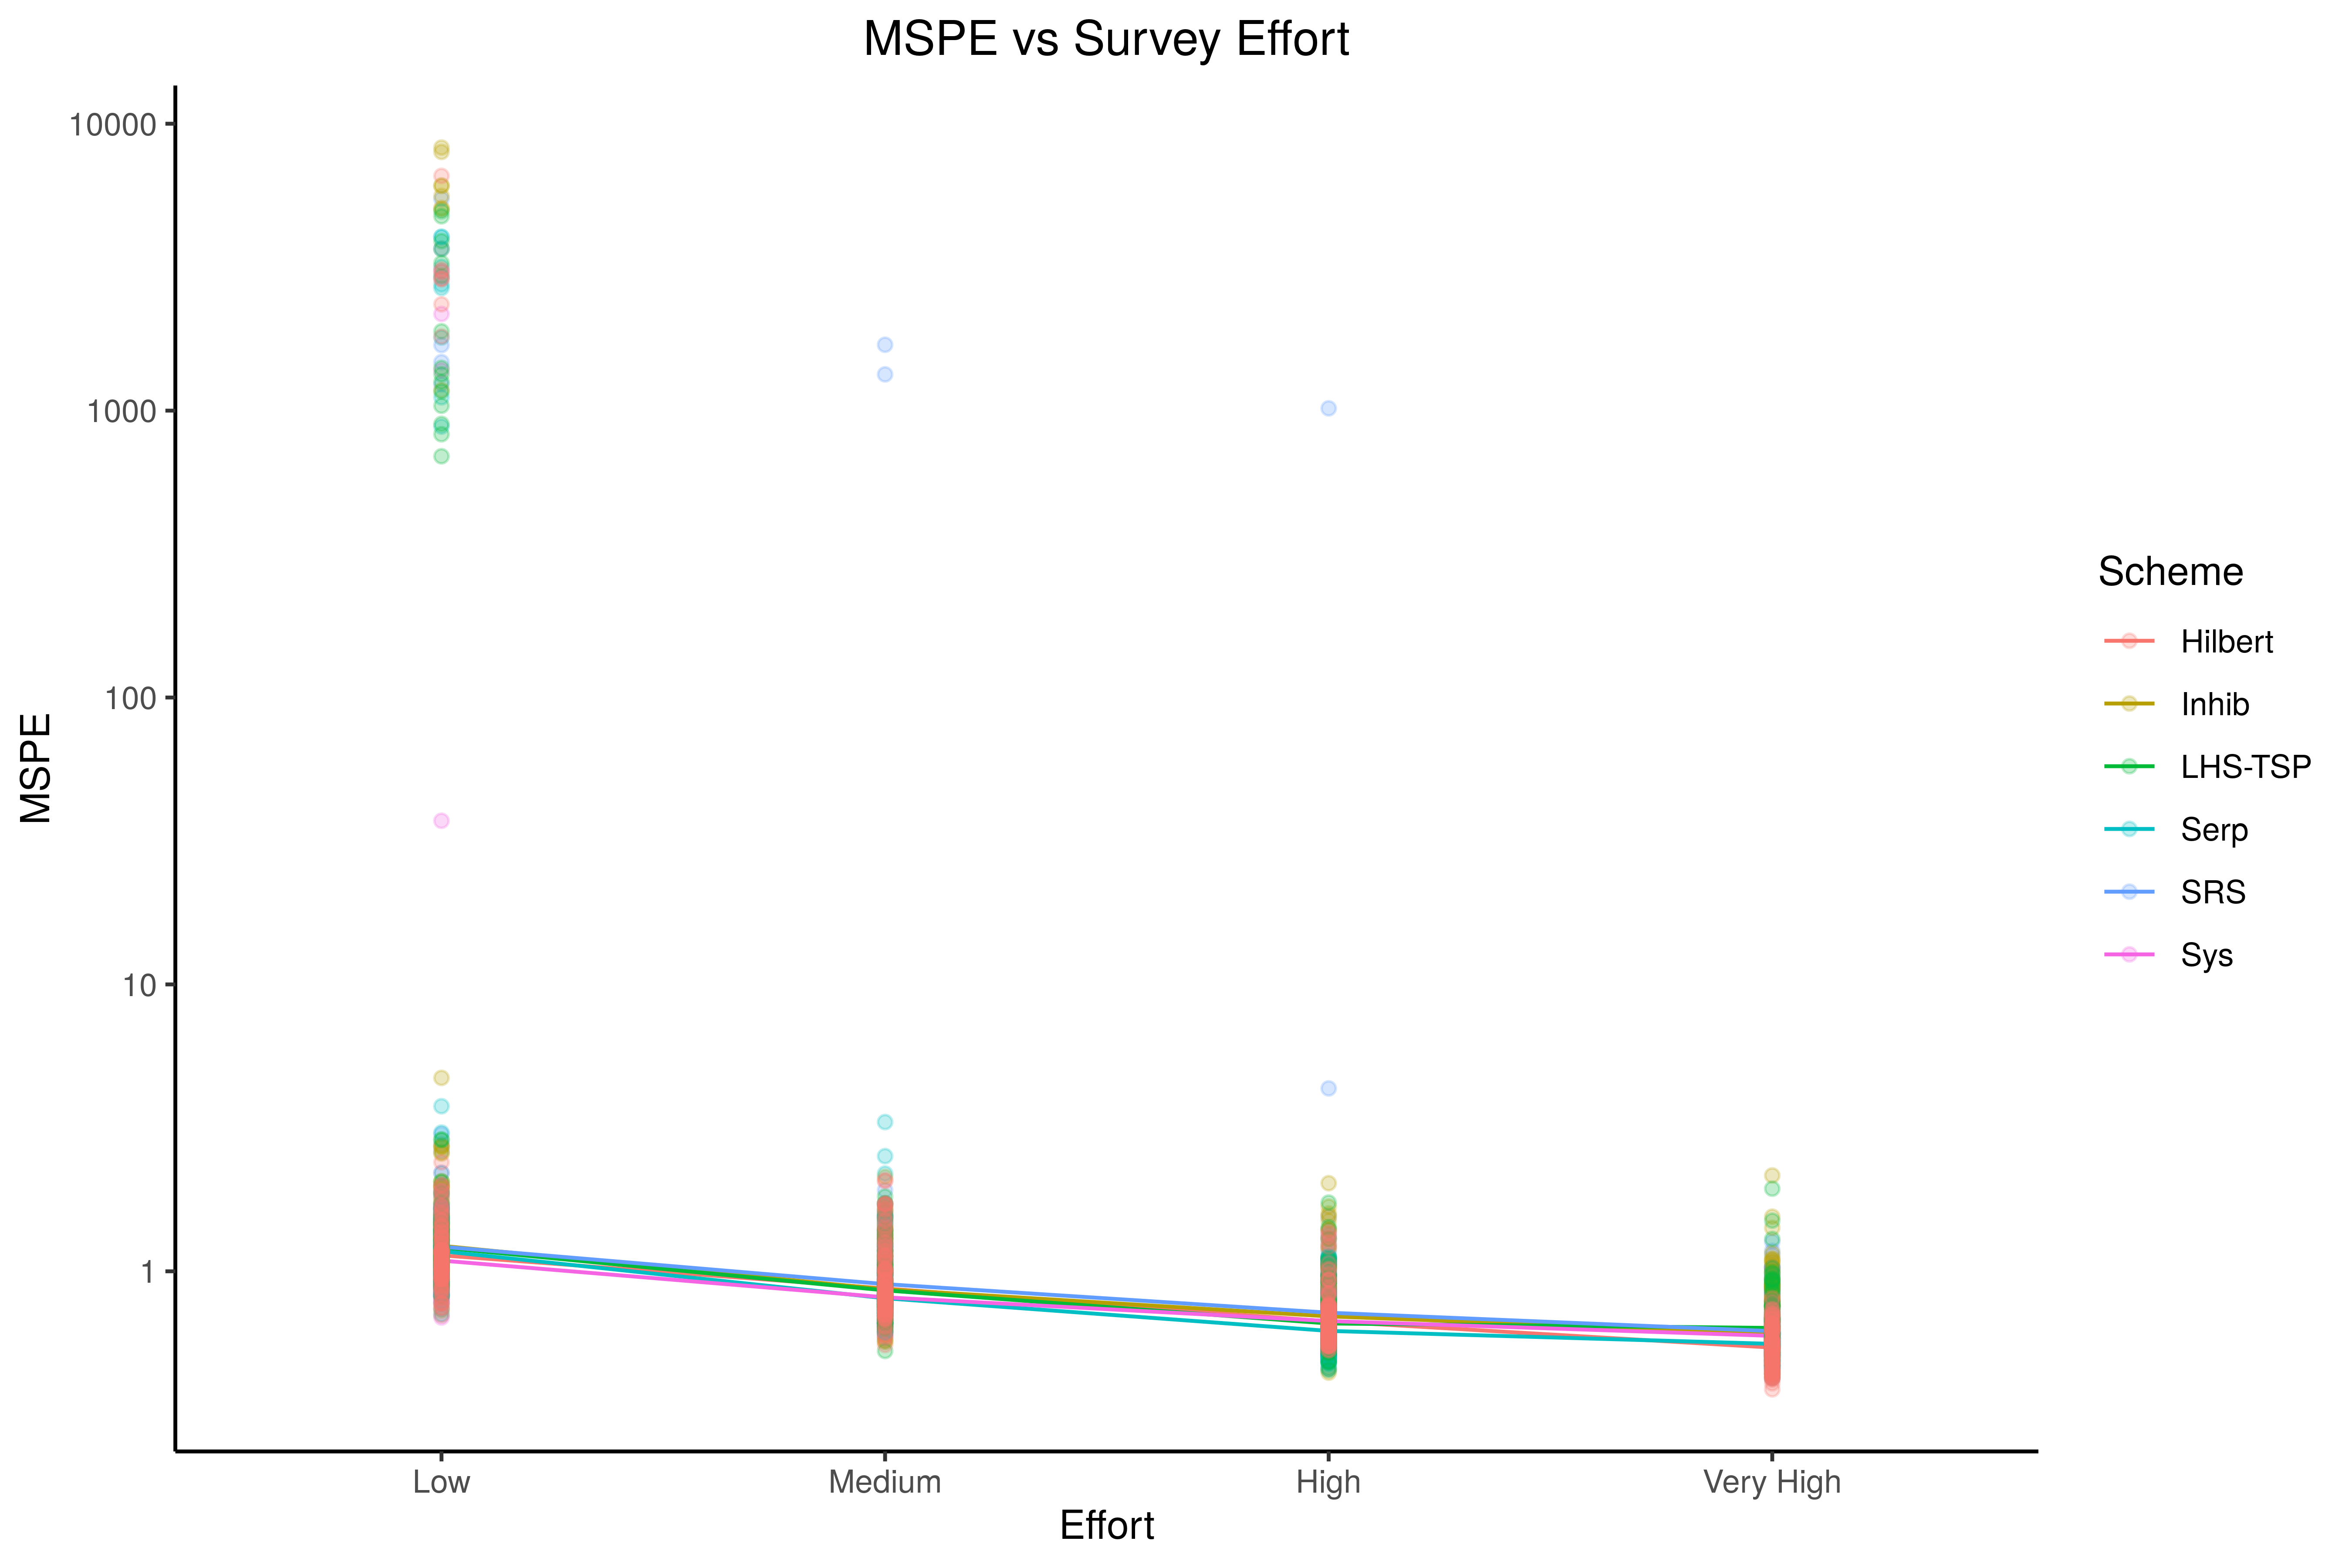
\includegraphics[width=4.5in]{../graphics/MSPE-effort-notpaneled-Cluster000004.png}
\caption{MSPE vs survey effort for one LGCP with Clusters dataset}
\label{mspeclust}
\end{subfigure}

\begin{subfigure}{4.5in}
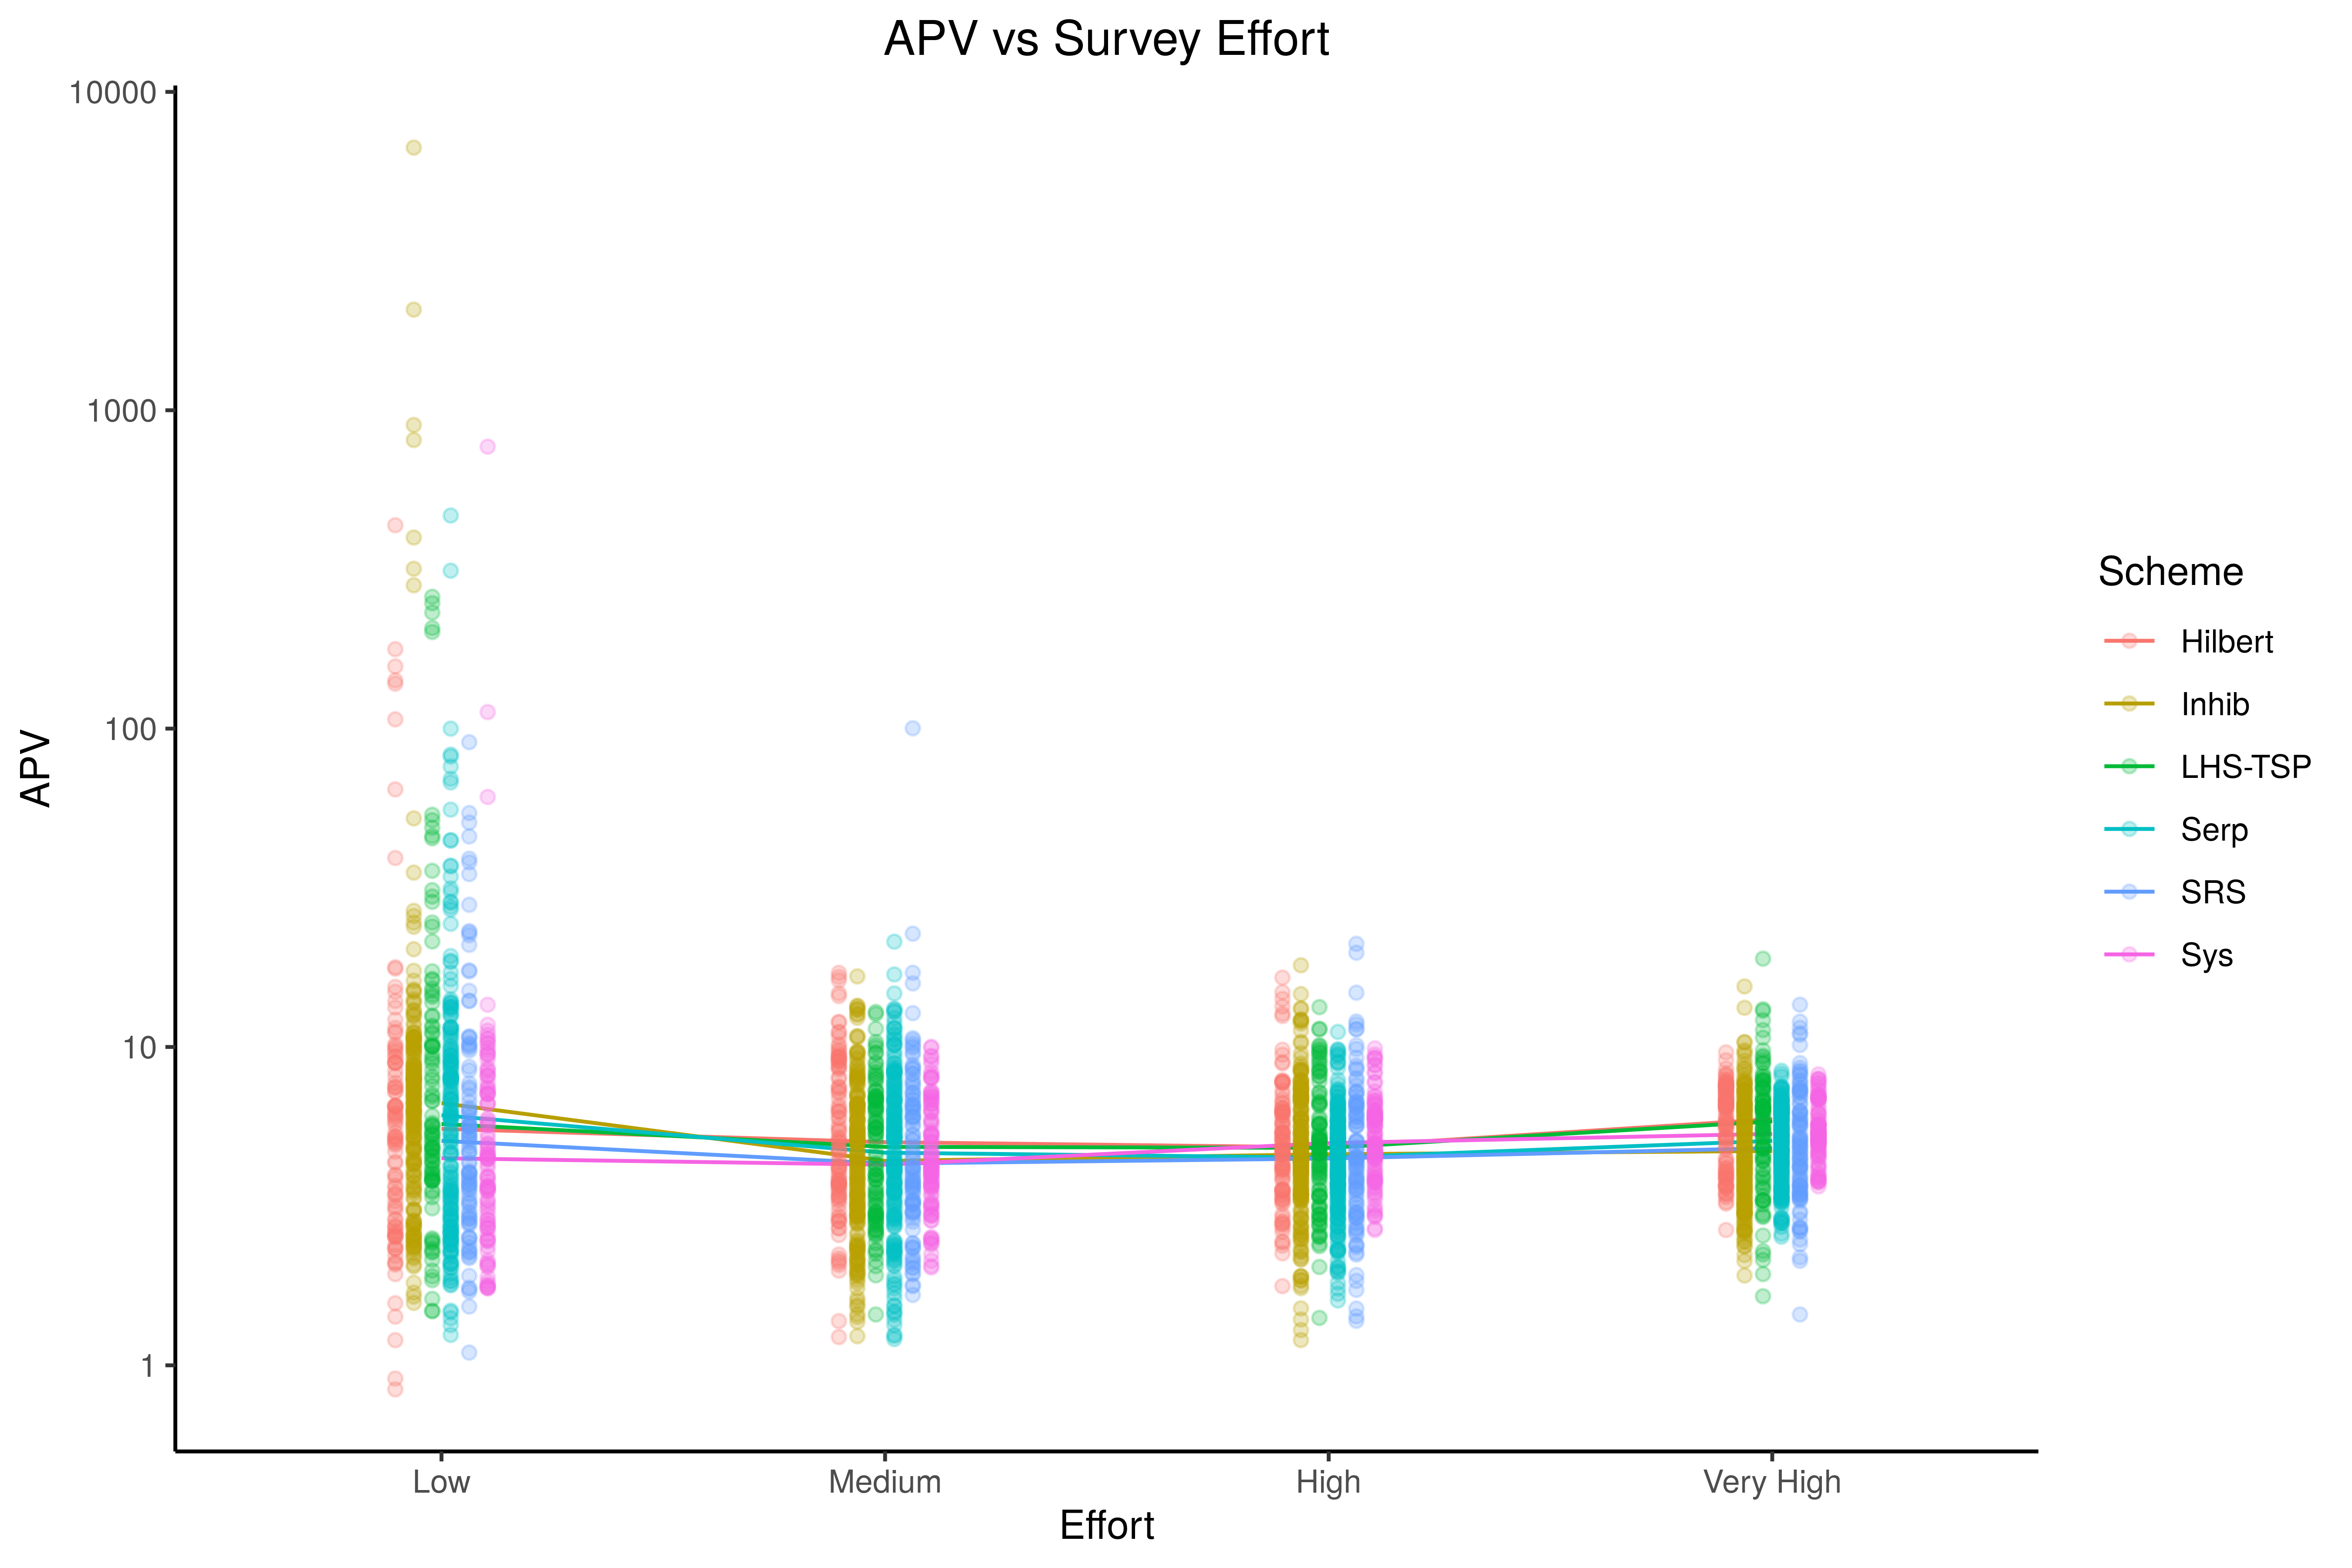
\includegraphics[width=4.5in]{../graphics/APV-effort-notpaneled-Cluster000004.png}
\caption{APV vs survey effort for one LGCP with Clusters dataset}
\label{apvclust}
\end{subfigure}

\caption{Plots of mean squared prediction error (MSPE) and average prediction
variance (APV) vs survey effort for each plan applied to one LGCP with Clusters
dataset. Line segments connect the median at each effort level.}
\label{clustresults}
\end{figure}


\subsection{Spatial coverage}

While the above results suggest the choice of design is relatively unimportant
and the distance traveled is the main driver of the quality of the spatial
predictions, it is important to consider that all of the design schemes ensure
the path is distributed across the entire study region. Designs that leave
large unexplored voids will not perform as well.

As an example, Figure~\ref{badxsect} shows the results of using a systematic
sample of 50 parallel transects in the western 20\% of the study site. This
design is the same length as our high-effort designs, but it leaves most of the
site far from the surveyed path. As a result, the predicted log-intensity is
flat near the GP posterior mean of \(-8.71\) over most of the site, rendering
the prediction mostly useless.

The problem with this example is easily explained in terms of the average
distance between the path and arbitrary points in the study site. This example
design has an average distance from the path of 486 units; the designs used in
the simulation study all had average distances to the path under 130 (with most
under 50). In the simulation study, there was little association between
MSPE and average distance to the path for paths of comparable length, but the
average distance to path decreased as effort (length) increased
(Figure \ref{covg}). This means that all of these schemes do well at
distributing the path around the site at all of these effort levels.

\begin{figure}

\begin{subfigure}{5in}
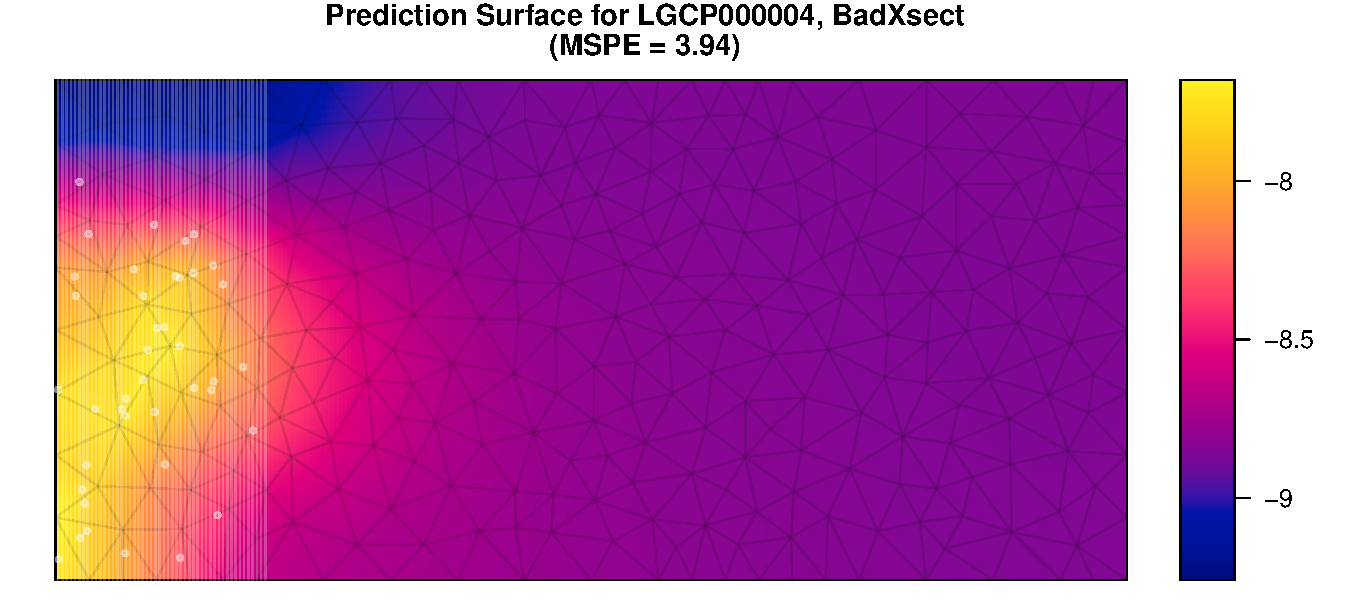
\includegraphics[width=5in]{../graphics/lambda-BadXsect-LGCP000004.pdf}
\caption{Predicted log-intensity}
\label{lambdabad}
\end{subfigure}

\begin{subfigure}{5in}
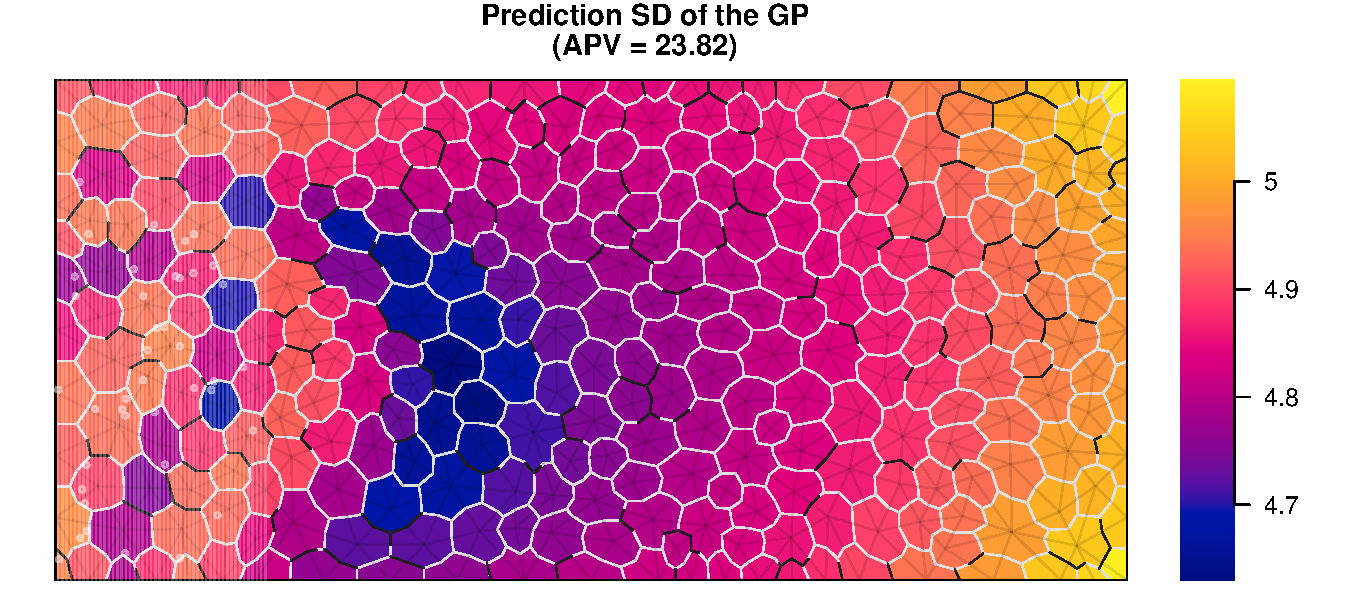
\includegraphics[width=5in]{../graphics/lambdaSD-BadXsect-LGCP000004.pdf}
\caption{Prediction SD}
\label{sdbad}
\end{subfigure}

\caption{Predicted log-intensity function and prediction standard deviation
using data observed via a systematic sample of a small section of the site. The
SD is shown for each finite element node.}
\label{badxsect}
\end{figure}


\begin{figure}

\begin{subfigure}{4.5in}
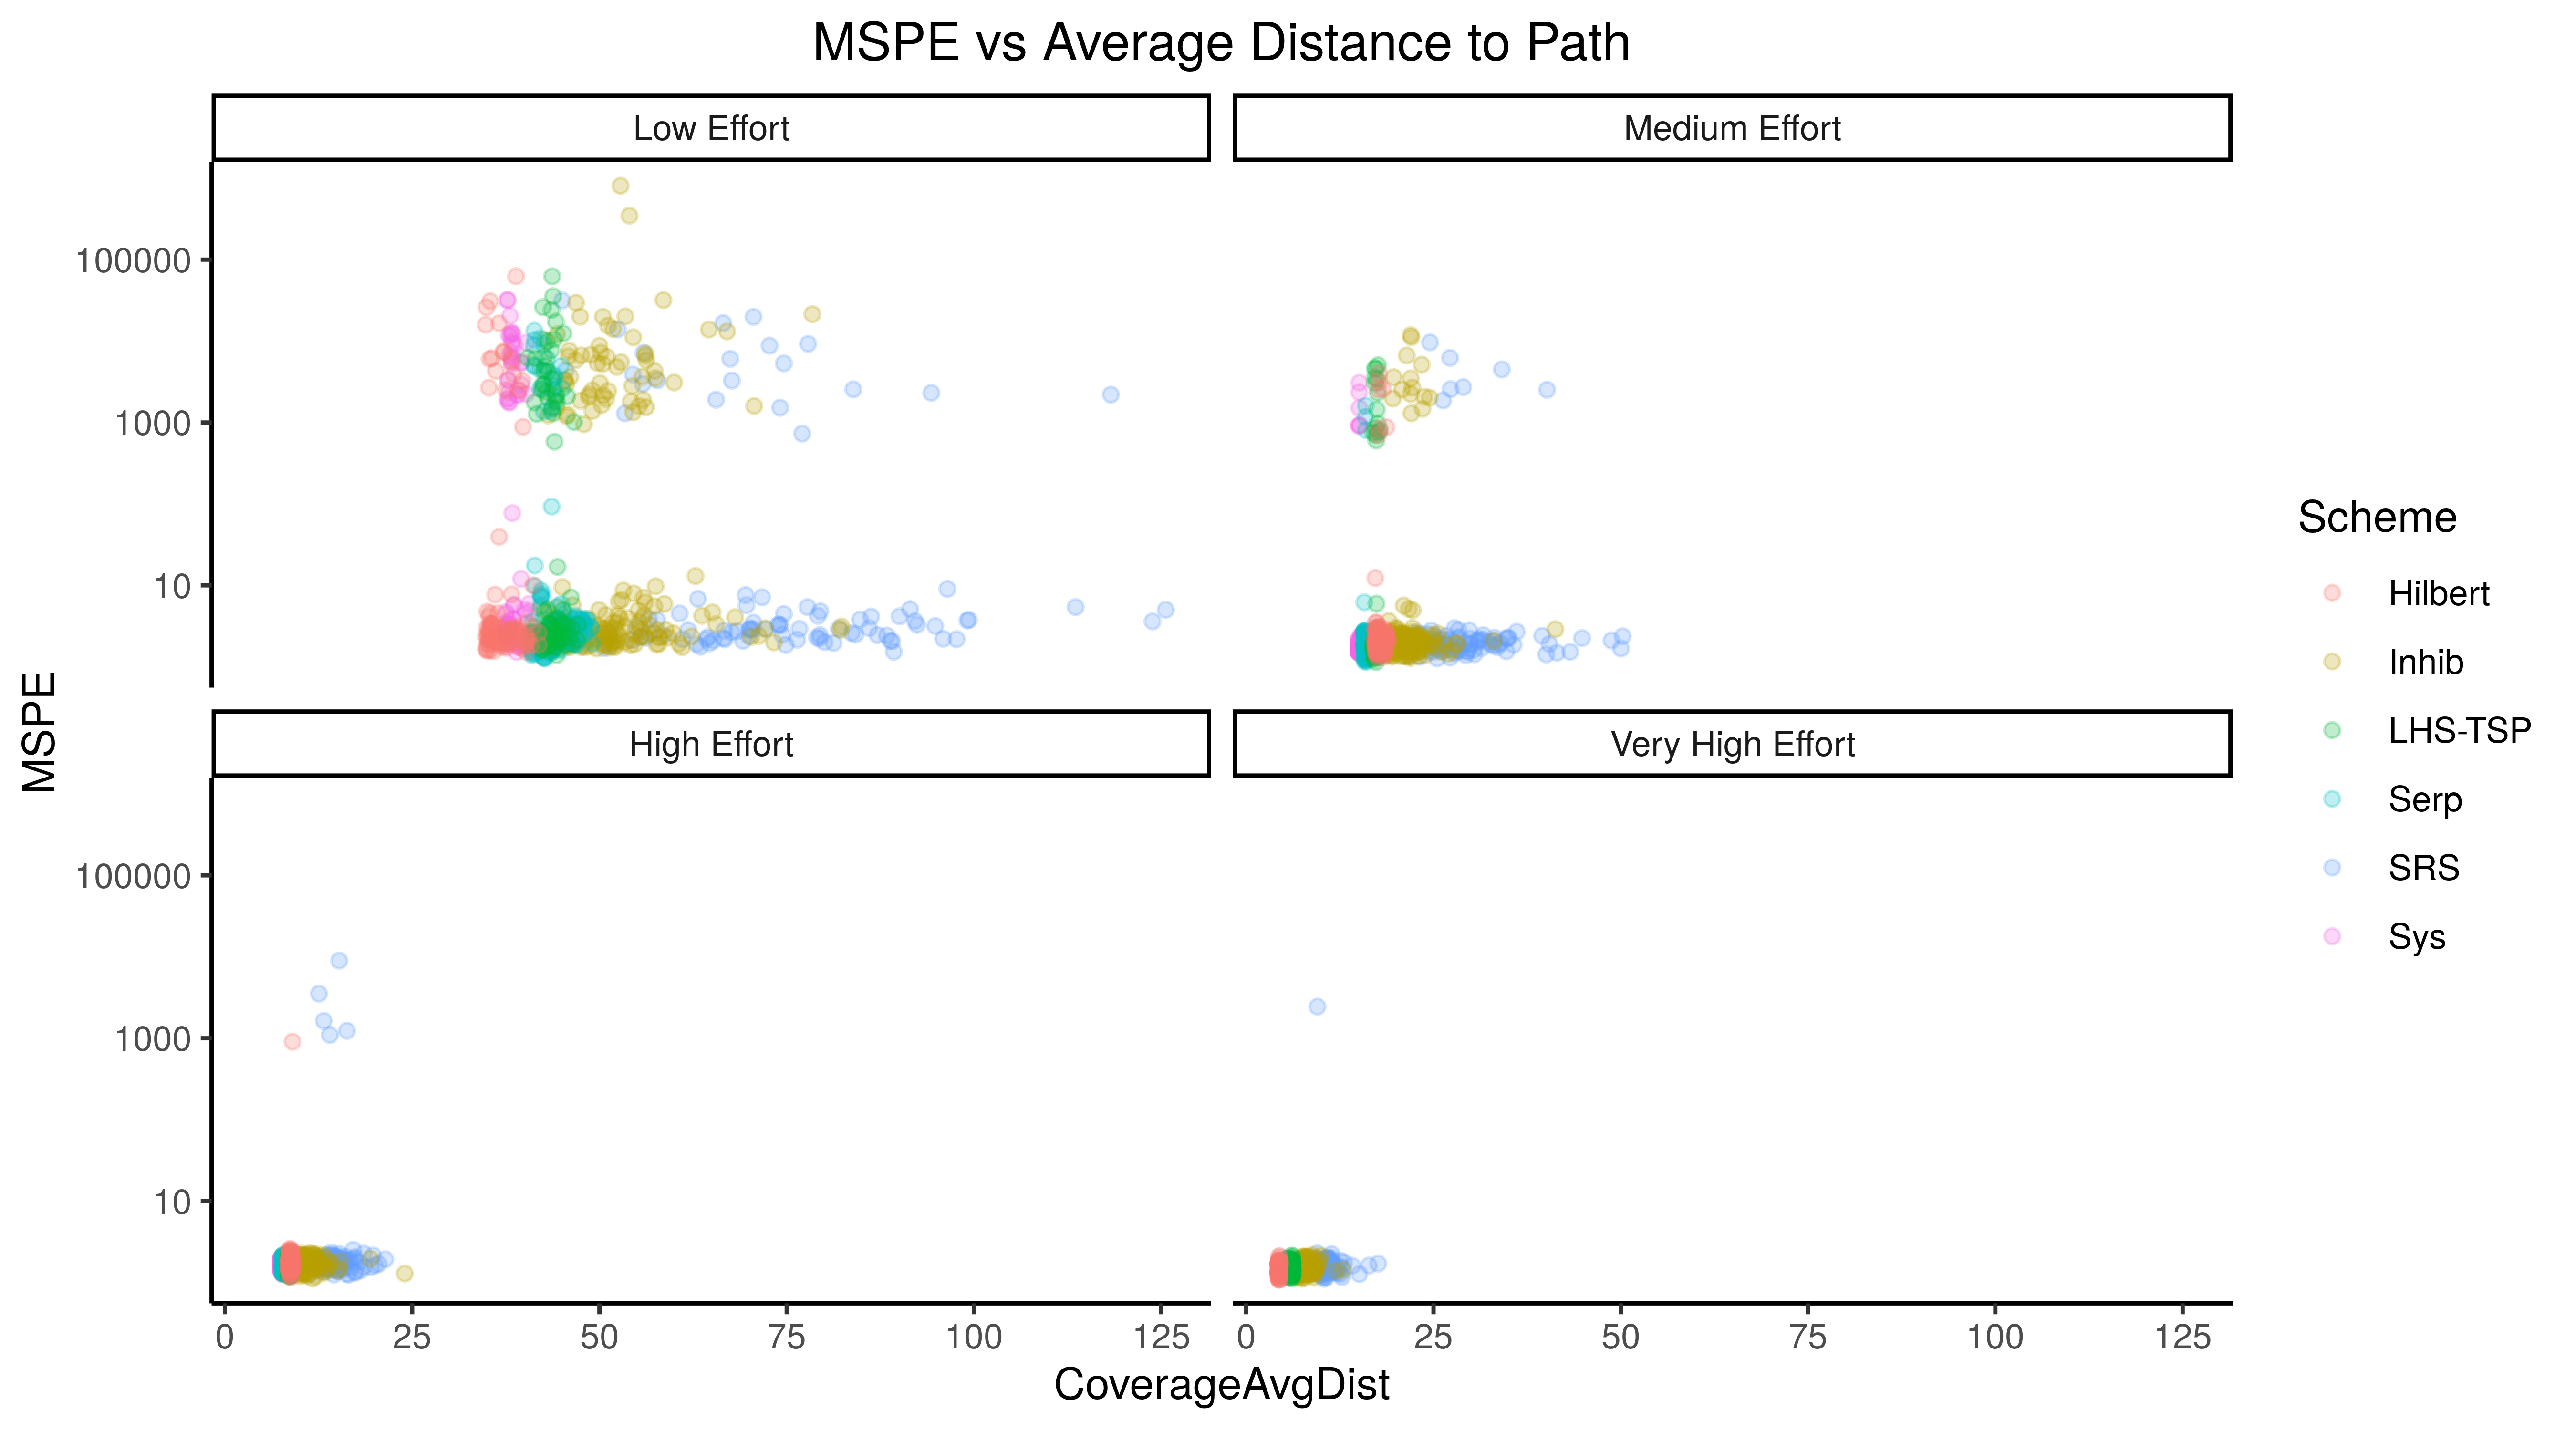
\includegraphics[width=4.5in]{../graphics/MSPE-Coverage-LGCP000004.png}
\caption{MSPE vs coverage for one LGCP dataset}
\label{covglgcp}
\end{subfigure}

\begin{subfigure}{4.5in}
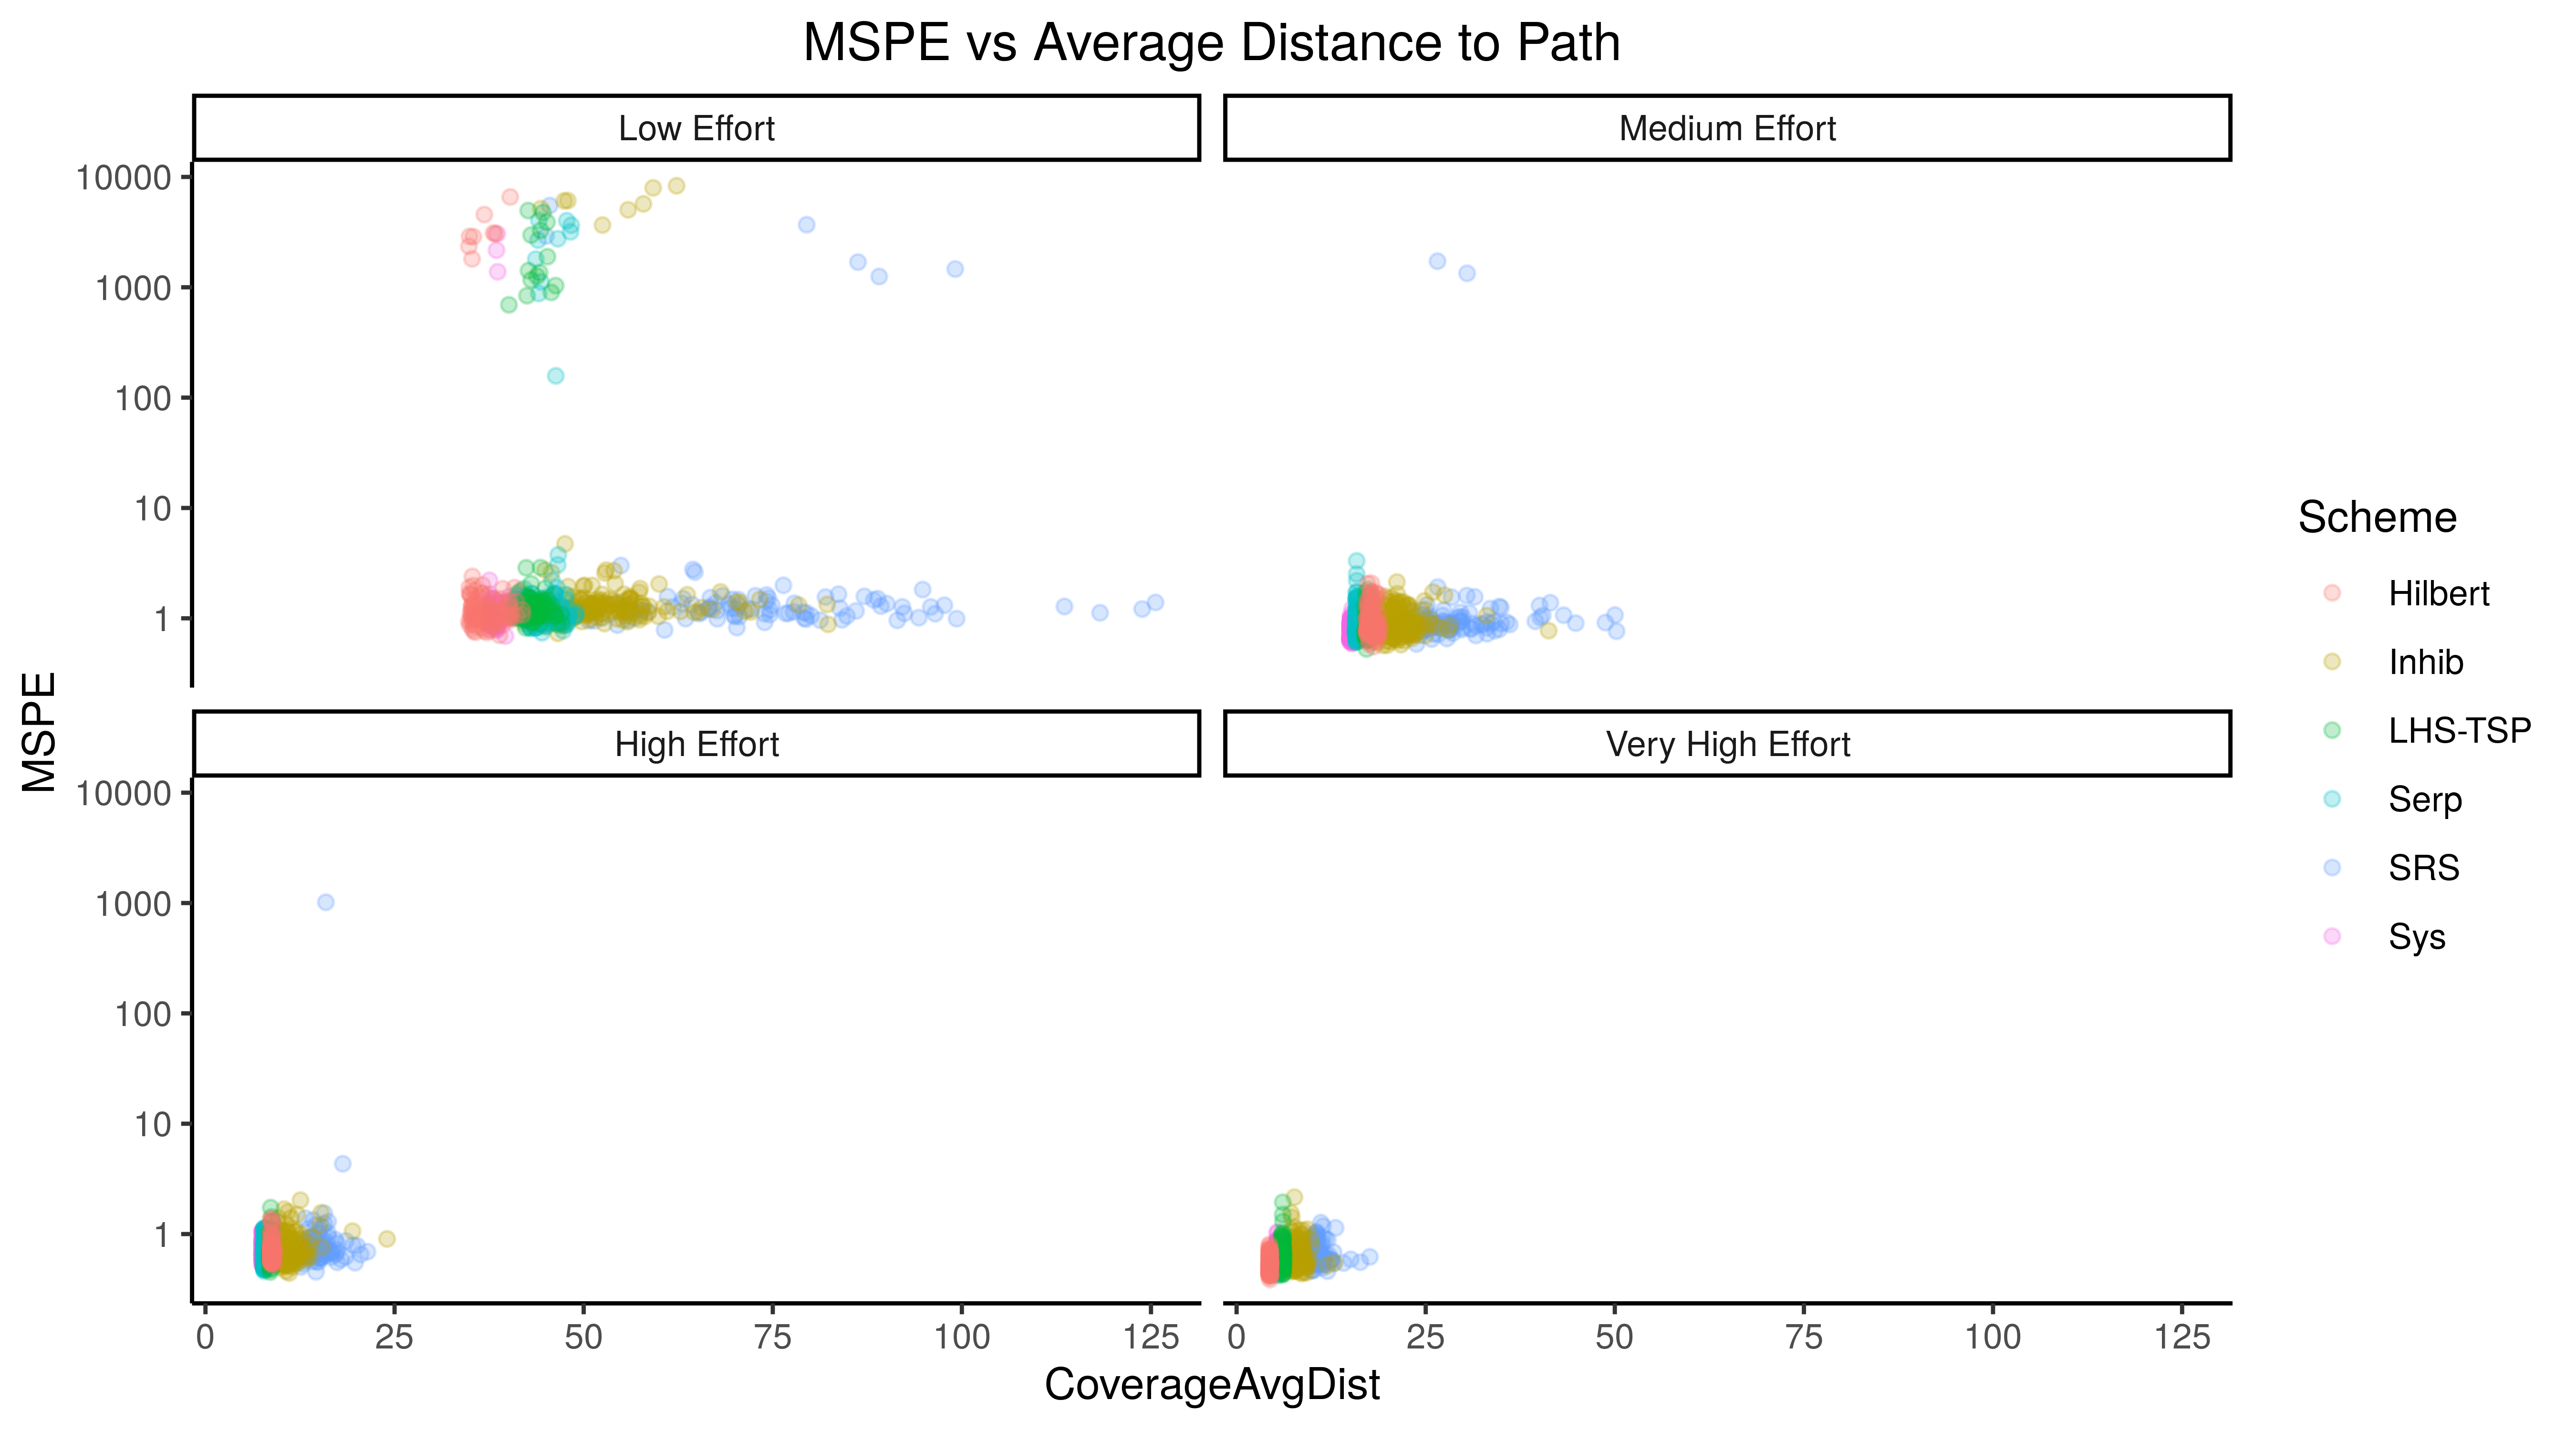
\includegraphics[width=4.5in]{../graphics/MSPE-Coverage-Cluster000004.png}
\caption{MSPE vs coverage for one LGCP with Clusters dataset}
\label{covgclust}
\end{subfigure}

\caption{MSPE plotted against the average distance from points in the site to
the nearest point on the path. As survey effort increases, the cloud of points
drifts down (lower MSPE) and to the left (lower average distance to the path).}
\label{covg}
\end{figure}

% Further things to plot:
% MSPE vs number of segments - Decreasing variability, no improvement after some point.
% MSPE vs average distance from path - linear relationship, varies by realization.
% Neither has a relationship with APV.


%\subsection{Augmenting a poor-performing design}

%Even a poor-performing design could be used as a starting point for sequential
%design. As a simple illustration, we augment the design from
%Figure~\ref{hilb000053lgcp} with some additional sampling effort in the western
%part of the site, where the original design left a large void.
%The total distance surveyed increases from 8581 to 12261 units, while the
%predicted log-intensity surface is much more accurate (Figure~\ref{aug}).
%MSPE decreases from 9.98 to 1.44 and APV improves from 38.16 to 9.55.
%Across the site, the prediction standard deviation is lower than before, and
%is now highest around in the middle. If we were to continue adding segments to
%the path, giving some attention to the central portion of the site could further
%improve the prediction.

%\begin{figure}

%\begin{subfigure}{5in}
%\includegraphics[width=5in]{../graphics/lambda-maxMSPE-Hilbert000053-LGCP000004}
%\caption{Predicted log-intensity}
%\label{lambdahilb000053lgcp}
%\end{subfigure}

%\begin{subfigure}{5in}
%\includegraphics[width=5in]{../graphics/lambdaSD-maxMSPE-Hilbert000053-LGCP000004.pdf}
%\caption{Prediction SD}
%\label{sdhilb000053lgcp}
%\end{subfigure}

%\caption{Predicted log-intensity function and prediction standard deviation
%using data observed via a Hilbert design. The SD is shown for each finite
%element node. This example is a medium-effort plan applied to a LGCP dataset.}
%\label{hilb000053lgcp}
%\end{figure}

%\begin{figure}

%\begin{subfigure}{5in}
%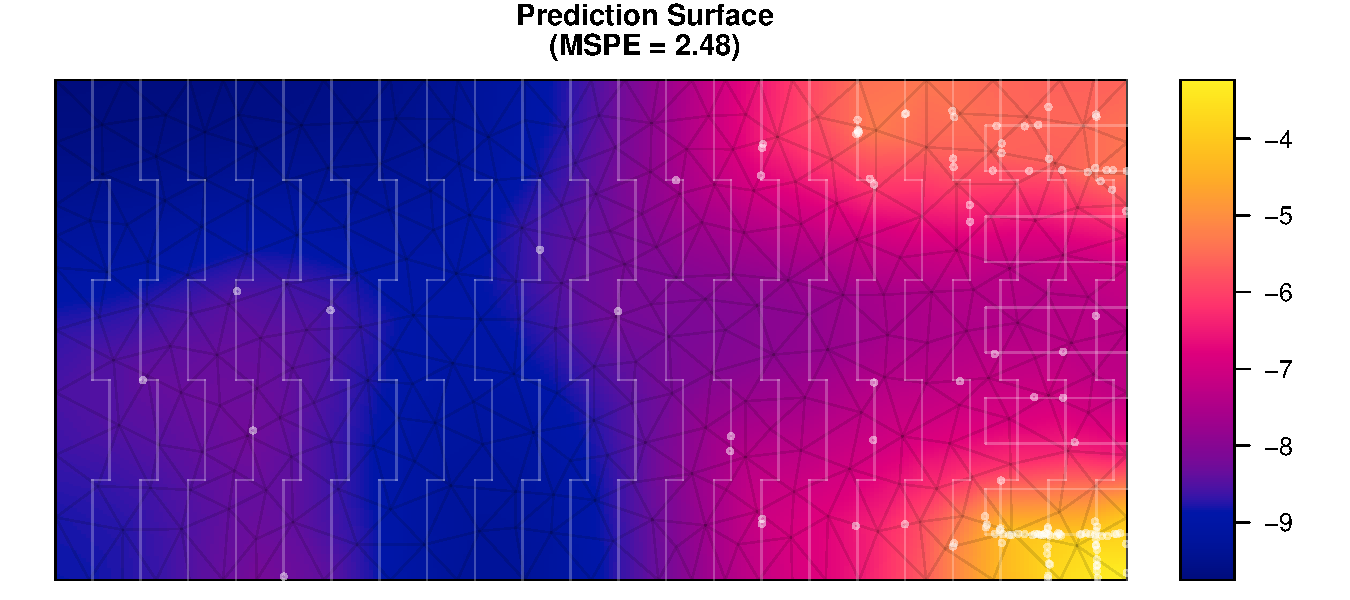
\includegraphics[width=5in]{../graphics/lambda-Aug-LGCP000004.pdf}
%\caption{Predicted log-intensity}
%\label{lambdaaug}
%\end{subfigure}

%\begin{subfigure}{5in}
%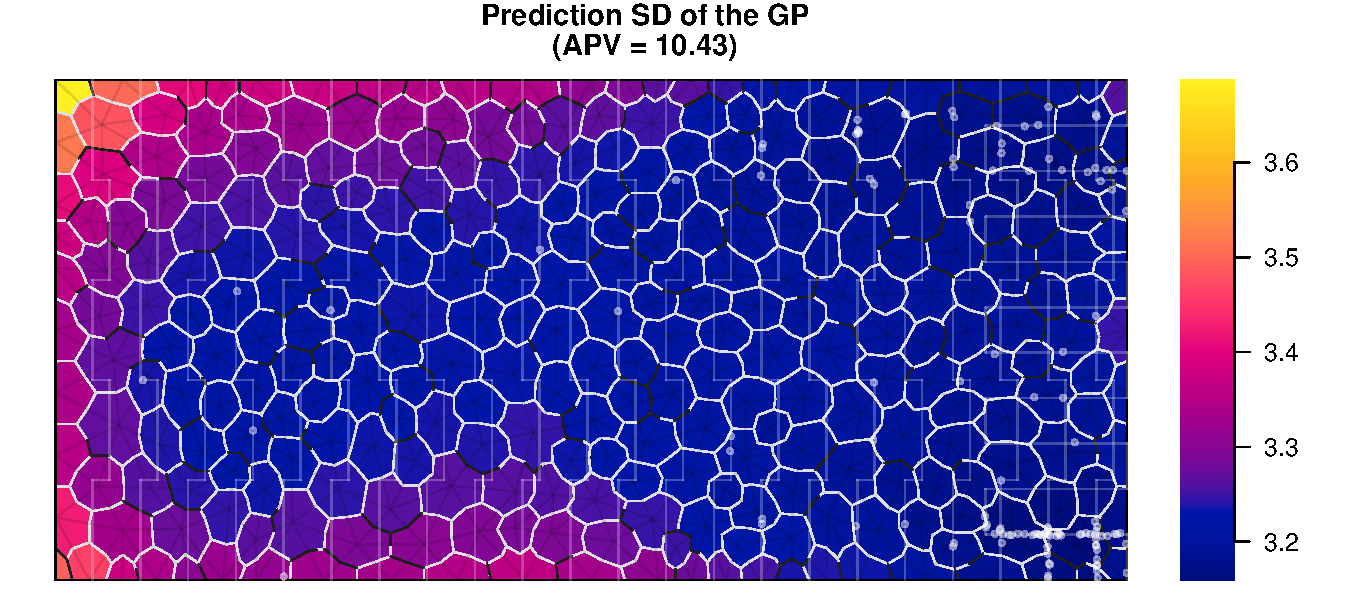
\includegraphics[width=5in]{../graphics/lambdaSD-Aug-LGCP000004.pdf}
%\caption{Prediction SD}
%\label{sdaug}
%\end{subfigure}

%\caption{Predicted log-intensity function and prediction standard deviation
%using data observed via a Hilber design augmented post-hoc. The SD is shown for
%each finite element node.}
%\label{aug}
%\end{figure}


\section{Discussion}
% This should explore the significance of the results of the work, not repeat them. A combined Results and Discussion section is often appropriate. Avoid extensive citations and discussion of published literature.

\subsection{Implications for sampling}

This study provides several insights about optimal sampling for LGCP models.
First of all, prediction uncertainty increases with distance from observed
\emph{events}, even along the path (consider the region of low posterior mean
and high standard deviation in the southwestern corner of
Figure~\ref{sdsrs000187clust}). This behavior is different from the behavior
of Gaussian process models in geostatistical studies, where observed design
points all provide information that reduces uncertainty of nearby predictions,
regardless of the values observed. In the LGCP model setting, an "observed"
strip that is observed to contain no events does not reduce the uncertainty in
nearby predictions. This is reasonable behavior with sparse sampling because
there may be events just out of detection range. Intuitively, observing no
events tells us the intensity should be ``low'' but says little about how low,
especially when intensity is modeled on a logarithmic scale.

This has consequences for adaptive or sequential design. A greedy algorithm
based entirely on minimizing variance may excessively sample regions of low
intensity, behavior that is unhelpful if the goal is to map hotspots of high
intensity. We recommend including design-based considerations of spatial
coverage in future studies on multi-stage design.

Additional considerations of applying path design to real-world studies include
practical issues of data collection. Generally the path will be smoothed,
without the perfectly-straight segments and instantaneous direction changes of
our simulated data collection. Equipment may have limitations which render
impossible the sharp corners of LHS-TSP designs or the repetitious short
segments and right angles of Hilbert curves. Future optimal design work could
incorporate turn angles into a loss function or use multi-objective
optimization~\citep{lark}.

% Of the schemes considered here, only the transect schemes allow the
% flexibility to set a desired path length and create a design of that length.


\subsection{Computing}

Bayesian computing (especially INLA) has brought LGCP models into the realm of
practicality. However, this is not yet a fully ``push button, get results''
procedure; in a handful of our simulations, the gradient descent step of INLA
failed to converge with the software's default settings. In many other
simulations, the posterior predictions appear numerically unstable at nodes on
the boundary.

One aspect that would affect both of these issues is the choice of finite
element mesh. A finer mesh than the one used in these simulations would have
more flexibility to model steep changes in the GP surface. We hypothesize that
this would make convergence problems and edge effects less likely. The downside
of a finer mesh is increased computing time because each mesh node becomes a
pseudodata point that must be processed by the model-fitting software. The
choice of mesh is non-trivial and worthy of further study.


\subsection{Conclusions}
% The main conclusions of the study may be presented in a short Conclusions section, which may stand alone or form a subsection of a Discussion or Results and Discussion section.

For optimal MSPE and APV, the choice of design scheme does not matter much as
long as it provides spatial coverage. For short paths, including corners and
regular spacing help avoid model-fitting problems, as in the Hilbert and
serpentine transect designs. On the other hand, systematic line-transect
designs provide the best spatial coverage but require many transects for good
model performance. There is a tradeoff between obtaining a useable posterior
and employing a simple design. We recommend the Hilbert or serpentine designs
if path length is heavily constrained, but systematic line transects are fine
if the path can be long. A simulation using available prior information for a
specific study will be helpful in assessing if a given length is ``long
enough'' to use a line-transect design.


\pagebreak
\appendix
\section{Profiles of designs across all datasets}
\label{profplots}

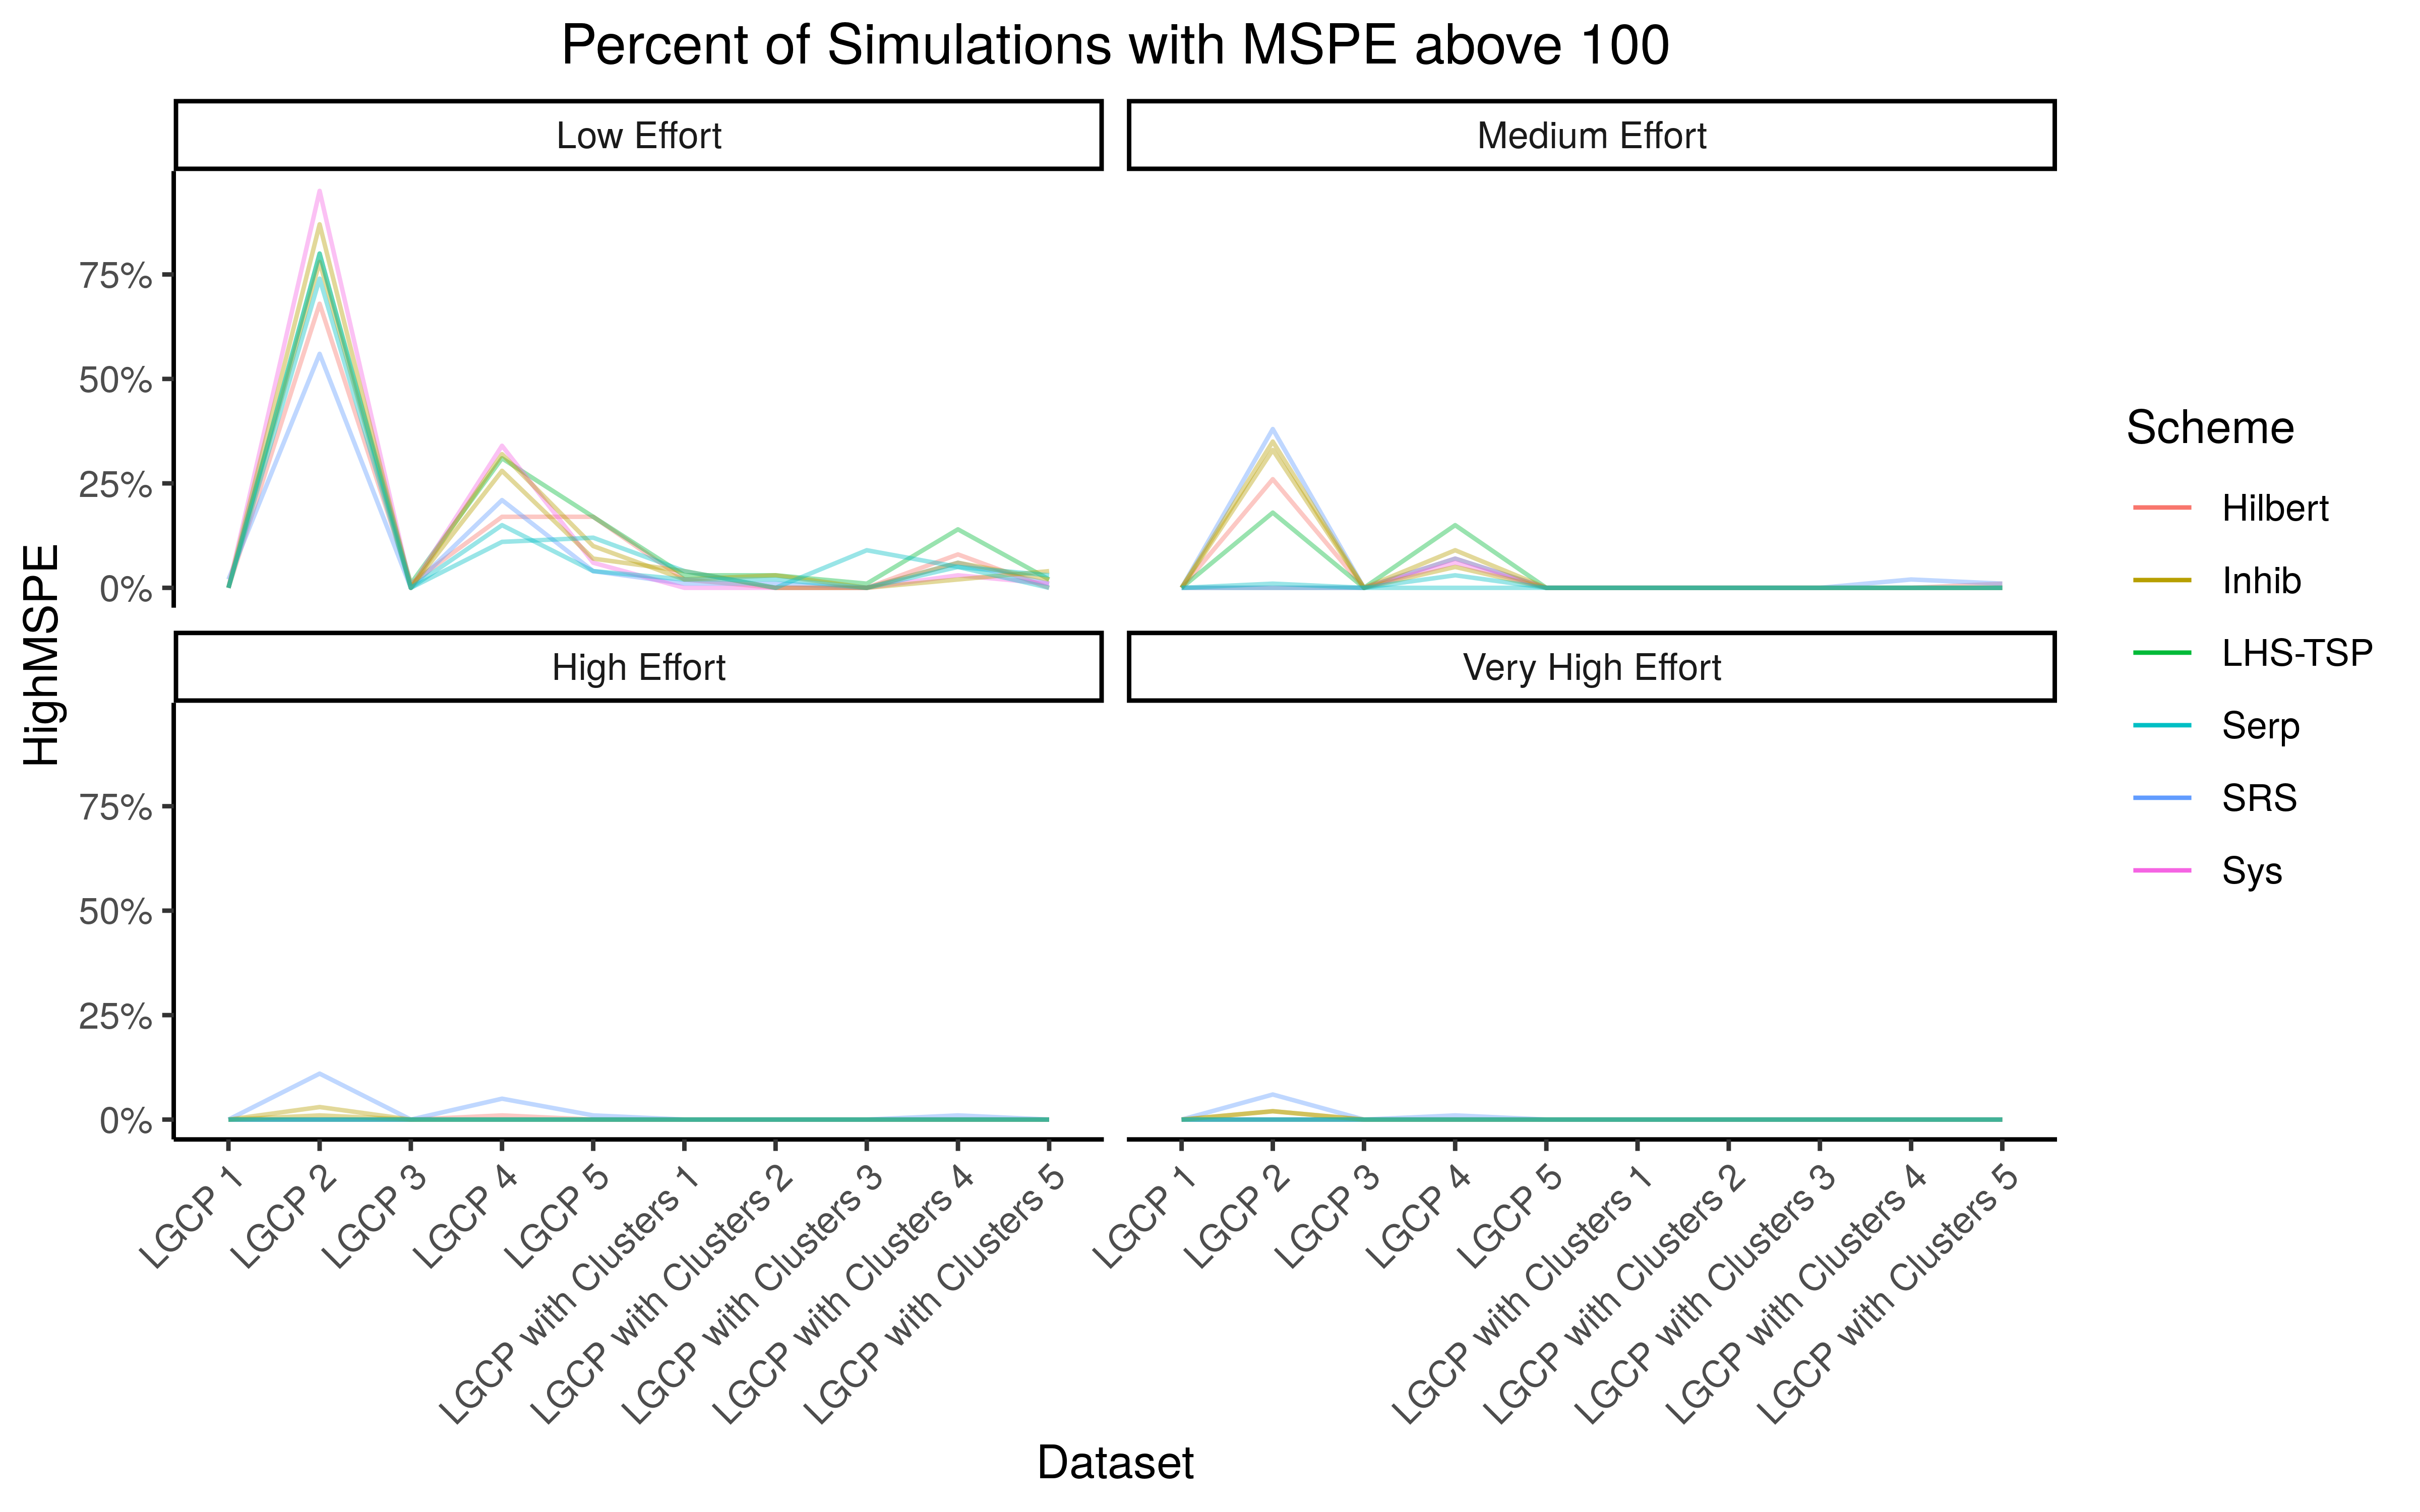
\includegraphics[width=4.5in]{../graphics/HighMSPE-profile.png}

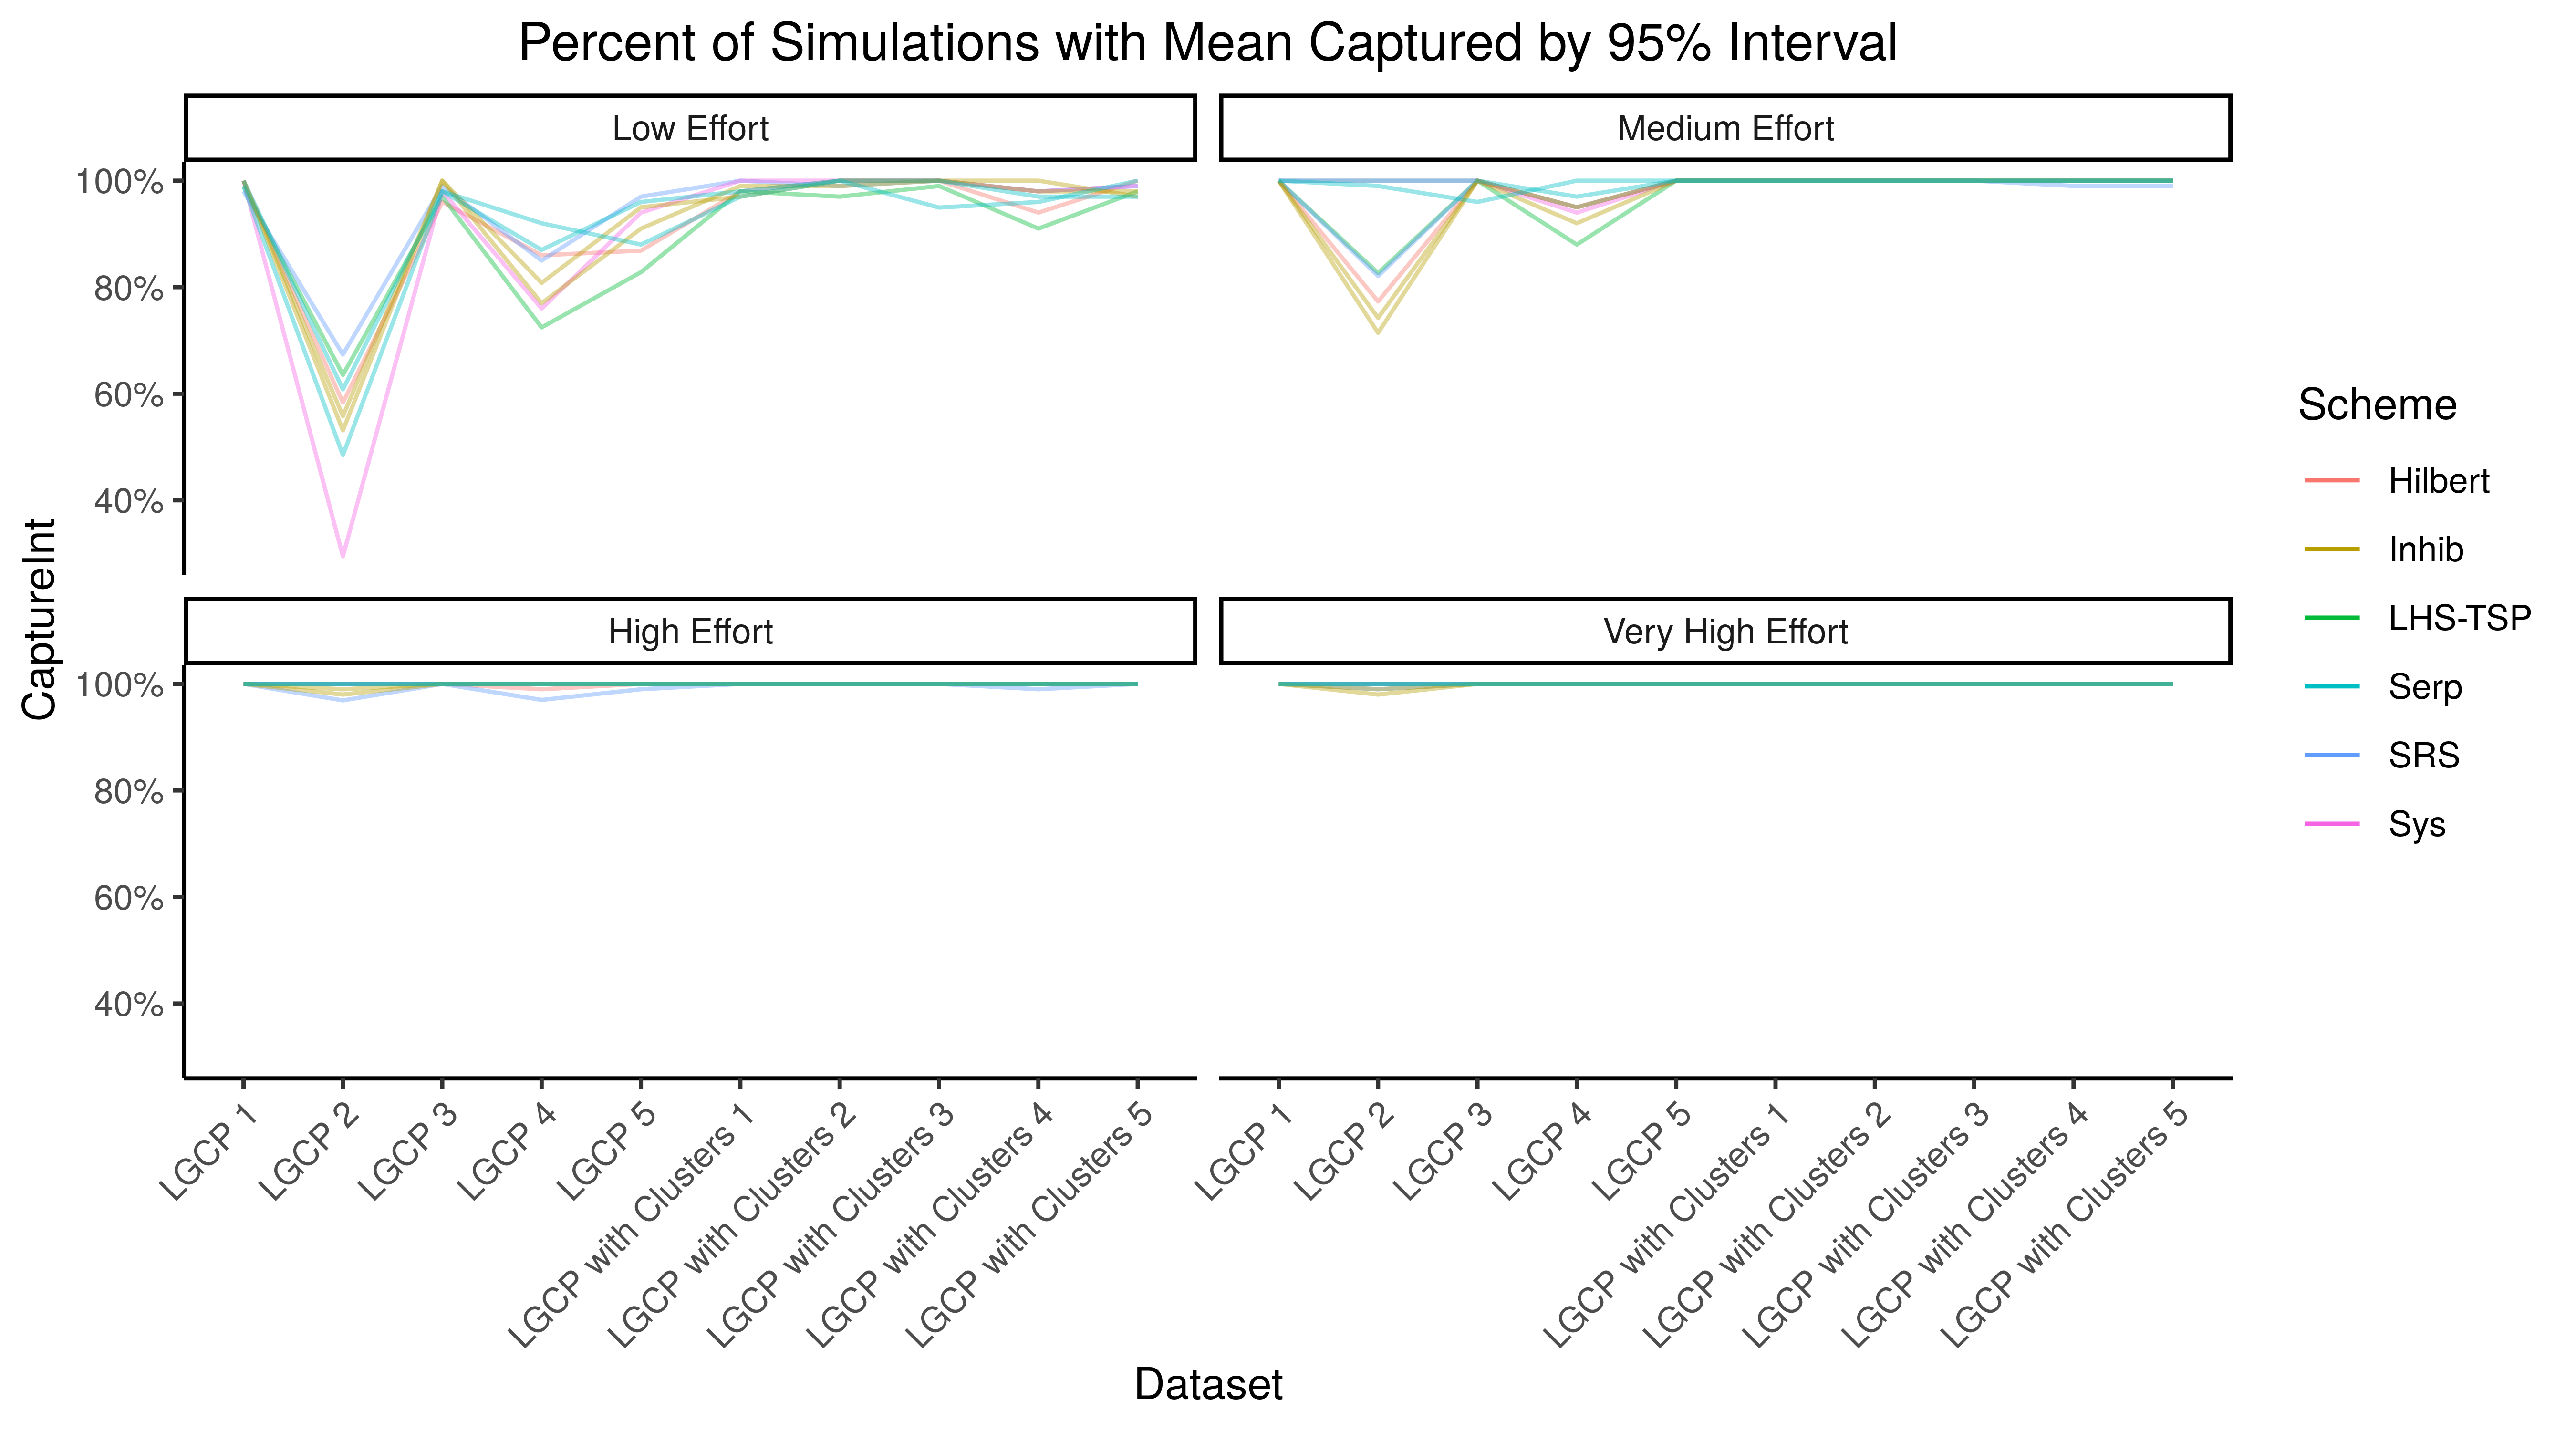
\includegraphics[width=4.5in]{../graphics/IntCapture-profile.png}

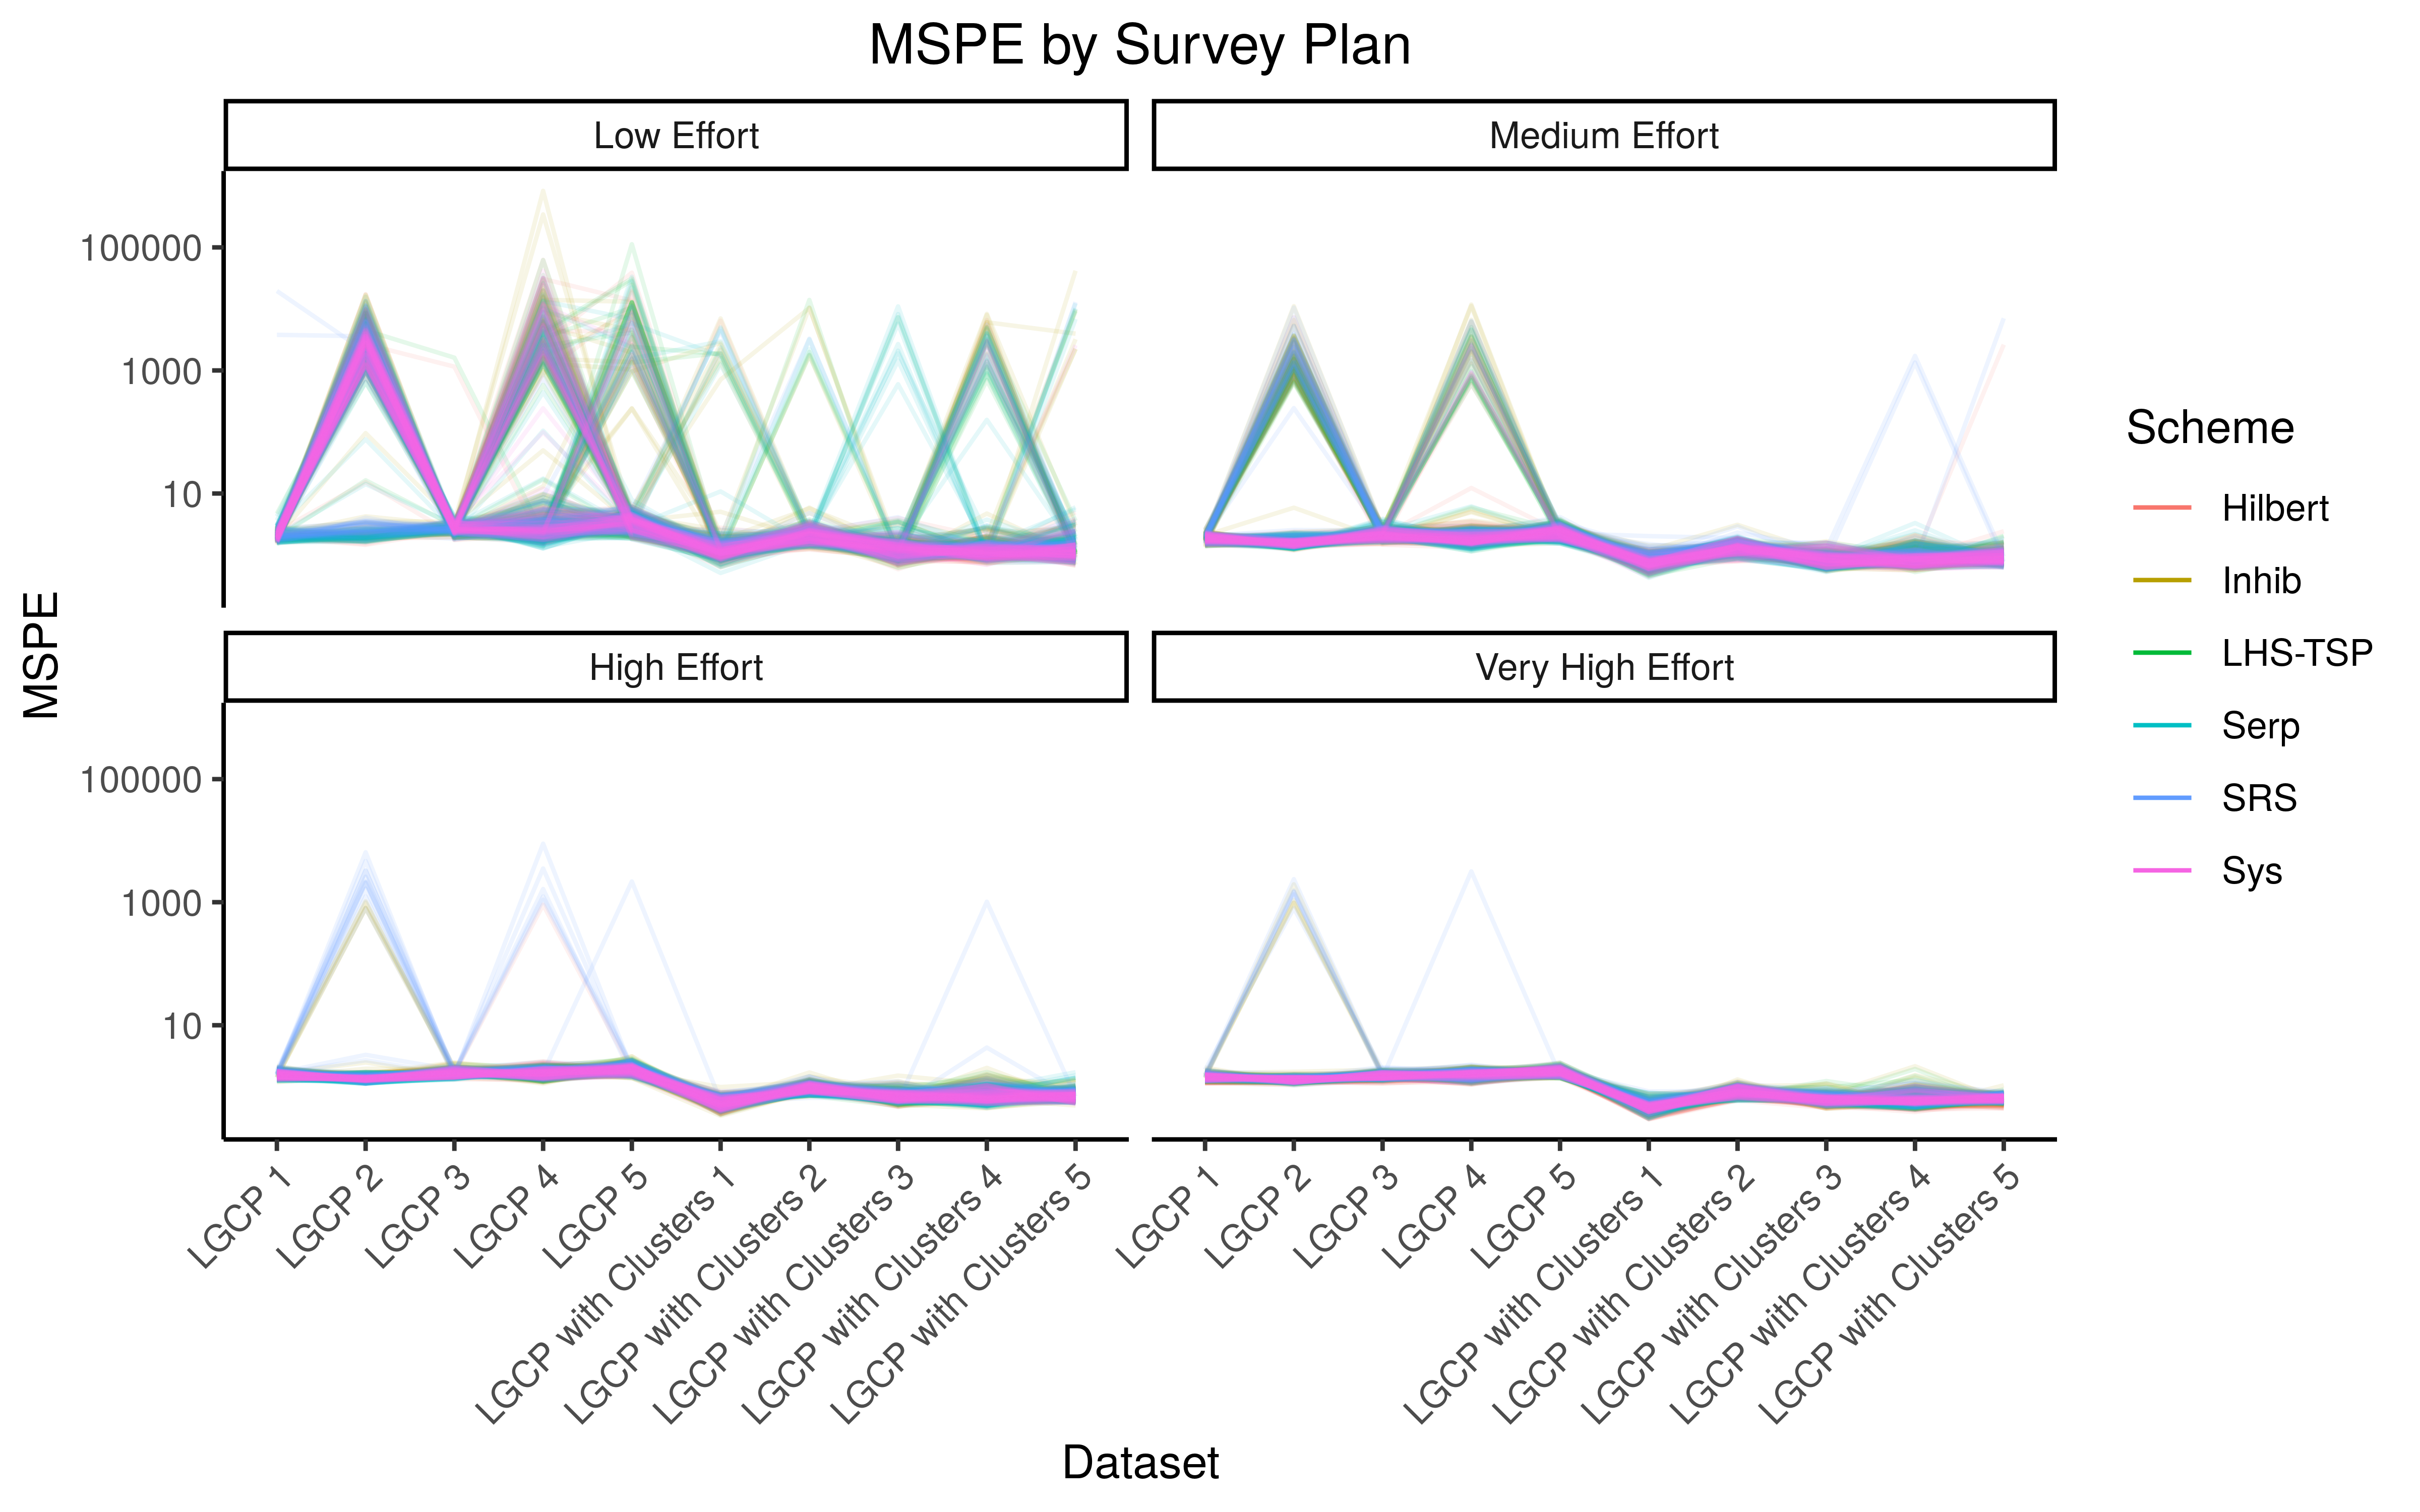
\includegraphics[width=4.5in]{../graphics/MSPE-profile.png}

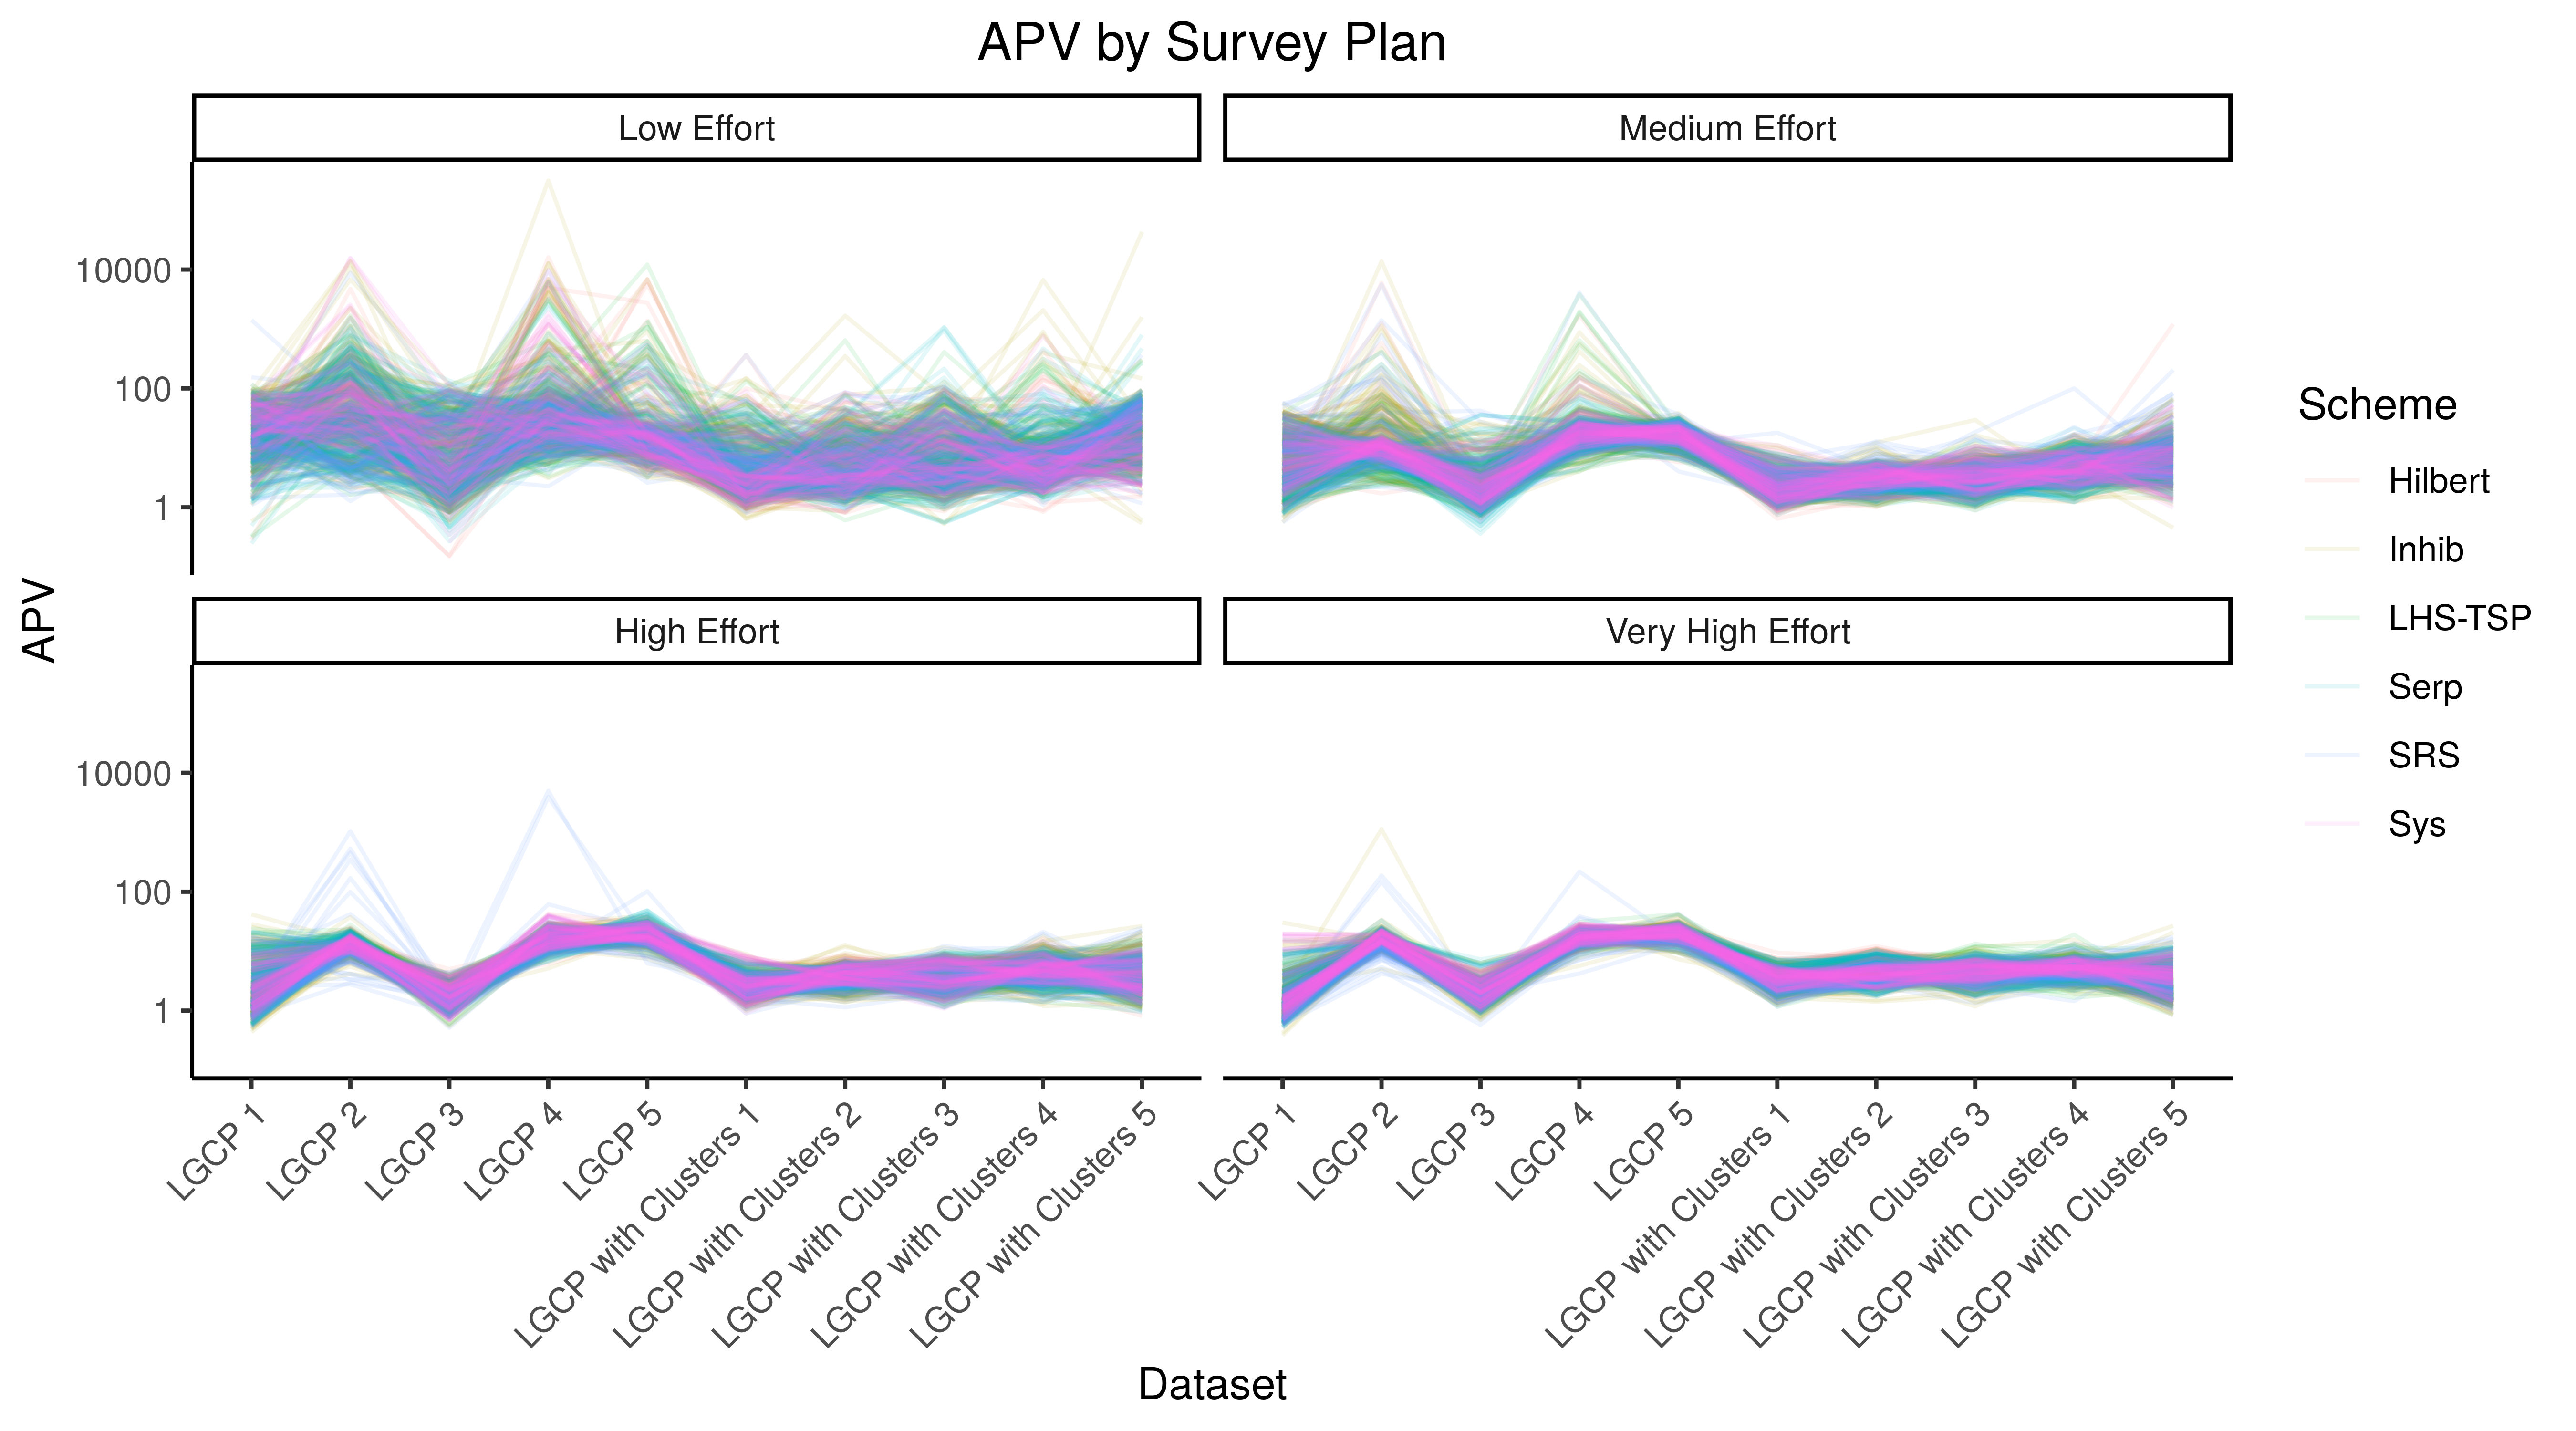
\includegraphics[width=4.5in]{../graphics/APV-profile.png}


\pagebreak
\section{Tables summarizing results}

%\subsection{LGCP dataset}

\begin{table}[h!]\tiny
\caption{Summary of model fitting and spatial prediction for each design
applied to a single LGCP dataset.}
\label{lgcptable}
\begin{tabular}{|l|c|c|c|c|cc|cc|}
\hline
& & Not & & Mean & \multicolumn{2}{|c|}{MSPE} & \multicolumn{2}{|c|}{APV} \\
Scheme & Effort & Converged & MSPE \(>\) 100 & Captured &
Median & IQR & Median & IQR \\
\hline
SRS &   Low & 0\% & 21\% &  85\% & 3.02 & 3.71  & 25.2 & 42.2  \\
&    Medium & 0\% &  7\% &  95\% & 1.90 & 0.593 & 16.2 & 10.6  \\
&      High & 0\% &  5\% &  97\% & 1.79 & 0.442 & 15.2 &  7.17 \\
& Very High & 0\% &  1\% & 100\% & 1.61 & 0.399 & 15.5 &  4.93 \\
\hline
Systematic & Low & 0\% & 34\% &  76\% & 3.29 & 2260  & 36.8 & 61.4 \\
&         Medium & 0\% &  6\% &  94\% & 1.75 & 0.370 & 18.4 & 10.2 \\
&           High & 0\% &  0\% & 100\% & 1.65 & 0.216 & 18.0 & 11.4 \\
&      Very High & 0\% &  0\% & 100\% & 1.62 & 0.158 & 17.3 &  5.27 \\
\hline
Inhibitory,      &    Low & 0\% & 32\% &  77\% & 3.02 & 2094  & 26.9 & 60.6  \\
10\% Close Pairs & Medium & 0\% &  5\% &  95\% & 1.96 & 0.570 & 16.7 & 10.7  \\
&                    High & 0\% &  0\% & 100\% & 1.73 & 0.367 & 16.7 &  5.70 \\
&               Very High & 0\% &  0\% & 100\% & 1.60 & 0.345 & 16.6 &  5.89 \\
\hline
Inhibitory,      &    Low & 1\% & 28\% &  80\% & 3.57 & 1290  & 32.2 & 46.5  \\
20\% Close Pairs & Medium & 0\% &  9\% &  92\% & 1.96 & 0.543 & 16.4 &  8.29 \\
&                    High & 0\% &  0\% & 100\% & 1.68 & 0.382 & 17.5 &  5.98 \\
&               Very High & 0\% &  0\% & 100\% & 1.59 & 0.289 & 17.2 &  5.07 \\
\hline
Serpentine, &  Low & 0\% & 11\% &  92\% & 2.37 & 1.33  & 27.9 & 35.6  \\
5 zigzags & Medium & 0\% &  3\% &  97\% & 1.88 & 0.350 & 13.9 &  9.26 \\
&             High & 0\% &  0\% & 100\% & 1.64 & 0.268 & 14.6 &  9.27 \\
&        Very High & 0\% &  0\% & 100\% & 1.55 & 0.123 & 16.9 &  2.87 \\
\hline
Serpentine &   Low & 0\% & 15\% &  87\% & 2.61 & 2.07  & 29.2 & 33.3  \\
8 zigzags & Medium & 0\% &  0\% & 100\% & 1.88 & 0.408 & 18.3 &  8.15 \\
&             High & 0\% &  0\% & 100\% & 1.64 & 0.245 & 17.6 &  6.25 \\
&        Very High & 0\% &  0\% & 100\% & 1.53 & 0.272 & 16.4 &  5.41 \\
\hline
LHS-TSP & Low & 2\% & 31\% &  71\% & 2.90 & 1777  & 22.9 & 57.5  \\
&      Medium & 0\% & 15\% &  88\% & 1.92 & 0.730 & 14.8 & 14.4  \\
&        High & 0\% &  0\% & 100\% & 1.64 & 0.335 & 15.8 &  6.80 \\
&   Very High & 0\% &  0\% & 100\% & 1.53 & 0.298 & 16.2 &  5.61 \\
\hline
Hilbert & Low & 0\% & 17\% &  86\% & 2.54 & 1.44  & 25.6 & 44.2  \\
&      Medium & 0\% &  7\% &  95\% & 2.10 & 0.748 & 16.7 &  7.96 \\
&        High & 0\% &  1\% &  99\% & 1.67 & 0.438 & 14.3 &  5.54 \\
&   Very High & 0\% &  0\% & 100\% & 1.46 & 0.388 & 15.6 &  4.57 \\
\hline
\end{tabular}
\end{table}

%\subsection{LGCP with Clusters dataset}

\begin{table}[h!]\tiny
\caption{Summary of model fitting and spatial prediction for each design
applied to a single LGCP with Clusters dataset.}
\label{clusttable}
\begin{tabular}{|l|c|c|c|c|cc|cc|}
\hline
& & Not & & Mean & \multicolumn{2}{|c|}{MSPE} & \multicolumn{2}{|c|}{APV} \\
Scheme & Effort & Converged & MSPE \(>\) 100 & Captured &
Median & IQR & Median & IQR \\
\hline
SRS &   Low & 0\% & 6\% &  98\% & 1.22  & 0.339 & 5.02 & 5.72 \\
&    Medium & 0\% & 2\% &  99\% & 0.902 & 0.219 & 4.32 & 3.89 \\
&      High & 0\% & 1\% &  99\% & 0.717 & 0.216 & 4.45 & 3.28 \\
& Very High & 0\% & 0\% & 100\% & 0.619 & 0.223 & 4.81 & 2.97 \\
\hline
Systematic &   Low & 0\% & 3\% &  98\% & 1.08  & 0.338  & 4.50 & 4.67 \\
&           Medium & 0\% & 0\% & 100\% & 0.812 & 0.199  & 4.27 & 2.85 \\
&             High & 0\% & 0\% & 100\% & 0.671 & 0.189  & 5.01 & 2.02 \\
&        Very High & 0\% & 0\% & 100\% & 0.596 & 0.0846 & 5.33 & 1.39 \\
\hline
Inhibitory, &         Low & 1\% & 6\% &  97\% & 1.20  & 0.326 & 6.93 & 6.78 \\
10\% Close Pairs & Medium & 0\% & 0\% & 100\% & 0.887 & 0.245 & 4.92 & 3.33 \\
&                    High & 0\% & 0\% & 100\% & 0.694 & 0.167 & 4.64 & 2.27 \\
&               Very High & 0\% & 0\% & 100\% & 0.599 & 0.144 & 4.47 & 2.21 \\
\hline
Inhibitory &          Low & 0\% & 2\% & 100\% & 1.23  & 0.287 & 6.42 & 3.59 \\
20\% Close Pairs & Medium & 0\% & 0\% & 100\% & 0.832 & 0.222 & 4.19 & 3.82 \\
&                    High & 0\% & 0\% & 100\% & 0.701 & 0.253 & 4.53 & 3.57 \\
&               Very High & 0\% & 0\% & 100\% & 0.630 & 0.204 & 5.08 & 2.91 \\
\hline
Serpentine, & Low  & 0\% & 5\% &  96\% & 1.22  & 0.364  & 6.35 & 8.95 \\
5 zigzags & Medium & 0\% & 0\% & 100\% & 0.808 & 0.259  & 4.32 & 4.28 \\
&             High & 0\% & 0\% & 100\% & 0.597 & 0.137  & 4.23 & 1.73 \\
&        Very High & 0\% & 0\% & 100\% & 0.530 & 0.0924 & 4.32 & 2.50 \\
\hline
Serpentine, &  Low & 0\% & 5\% &  97\% & 1.11  & 0.342  & 6.10 & 5.77 \\
8 zigzags & Medium & 0\% & 0\% & 100\% & 0.795 & 0.163  & 5.14 & 3.19 \\
&             High & 0\% & 0\% & 100\% & 0.643 & 0.235  & 4.61 & 2.75 \\
&        Very High & 0\% & 0\% & 100\% & 0.564 & 0.0621 & 5.48 & 1.65 \\
\hline
LHS-TSP & Low & 0\% & 14\% &  91\% & 1.21  & 0.374 & 5.73 & 8.92 \\
&      Medium & 0\% &  0\% & 100\% & 0.858 & 0.281 & 5.09 & 3.81 \\
&        High & 0\% &  0\% & 100\% & 0.658 & 0.160 & 4.75 & 3.12 \\
&   Very High & 0\% &  0\% & 100\% & 0.635 & 0.198 & 5.79 & 2.96 \\
\hline
Hilbert & Low & 0\% & 8\% &  94\% & 1.14  & 0.451 & 5.57 & 6.15 \\
&      Medium & 0\% & 0\% & 100\% & 0.871 & 0.358 & 5.02 & 5.03 \\
&        High & 0\% & 0\% & 100\% & 0.669 & 0.152 & 4.86 & 2.64 \\
&   Very High & 0\% & 0\% & 100\% & 0.542 & 0.138 & 5.95 & 2.82 \\
\hline
\end{tabular}
\end{table}


\clearpage
\section{Additional plots of posterior predictions}
\label{moreplots}

\subsection{Minimum-MSPE surfaces, LGCP dataset}

\includegraphics[width=2.5in]{../graphics/lambda-minMSPE-Hilbert000013-LGCP000004.pdf}
\includegraphics[width=2.5in]{../graphics/lambdaSD-minMSPE-Hilbert000013-LGCP000004.pdf}

\includegraphics[width=2.5in]{../graphics/lambda-minMSPE-Hilbert000105-LGCP000004.pdf}
\includegraphics[width=2.5in]{../graphics/lambdaSD-minMSPE-Hilbert000105-LGCP000004.pdf}

\includegraphics[width=2.5in]{../graphics/lambda-minMSPE-Hilbert000263-LGCP000004.pdf}
\includegraphics[width=2.5in]{../graphics/lambdaSD-minMSPE-Hilbert000263-LGCP000004.pdf}

\includegraphics[width=2.5in]{../graphics/lambda-minMSPE-Hilbert000307-LGCP000004.pdf}
\includegraphics[width=2.5in]{../graphics/lambdaSD-minMSPE-Hilbert000307-LGCP000004.pdf}

\includegraphics[width=2.5in]{../graphics/lambda-minMSPE-Inhib000040-LGCP000004.pdf}
\includegraphics[width=2.5in]{../graphics/lambdaSD-minMSPE-Inhib000040-LGCP000004.pdf}

\includegraphics[width=2.5in]{../graphics/lambda-minMSPE-Inhib000117-LGCP000004.pdf}
\includegraphics[width=2.5in]{../graphics/lambdaSD-minMSPE-Inhib000117-LGCP000004.pdf}

\includegraphics[width=2.5in]{../graphics/lambda-minMSPE-Inhib000222-LGCP000004.pdf}
\includegraphics[width=2.5in]{../graphics/lambdaSD-minMSPE-Inhib000222-LGCP000004.pdf}

\includegraphics[width=2.5in]{../graphics/lambda-minMSPE-Inhib000378-LGCP000004.pdf}
\includegraphics[width=2.5in]{../graphics/lambdaSD-minMSPE-Inhib000378-LGCP000004.pdf}

\includegraphics[width=2.5in]{../graphics/lambda-minMSPE-Inhib000423-LGCP000004.pdf}
\includegraphics[width=2.5in]{../graphics/lambdaSD-minMSPE-Inhib000423-LGCP000004.pdf}

\includegraphics[width=2.5in]{../graphics/lambda-minMSPE-Inhib000512-LGCP000004.pdf}
\includegraphics[width=2.5in]{../graphics/lambdaSD-minMSPE-Inhib000512-LGCP000004.pdf}

\includegraphics[width=2.5in]{../graphics/lambda-minMSPE-Inhib000679-LGCP000004.pdf}
\includegraphics[width=2.5in]{../graphics/lambdaSD-minMSPE-Inhib000679-LGCP000004.pdf}

\includegraphics[width=2.5in]{../graphics/lambda-minMSPE-Inhib000794-LGCP000004.pdf}
\includegraphics[width=2.5in]{../graphics/lambdaSD-minMSPE-Inhib000794-LGCP000004.pdf}

\includegraphics[width=2.5in]{../graphics/lambda-minMSPE-LHS-TSP000034-LGCP000004.pdf}
\includegraphics[width=2.5in]{../graphics/lambdaSD-minMSPE-LHS-TSP000034-LGCP000004.pdf}

\includegraphics[width=2.5in]{../graphics/lambda-minMSPE-LHS-TSP000103-LGCP000004.pdf}
\includegraphics[width=2.5in]{../graphics/lambdaSD-minMSPE-LHS-TSP000103-LGCP000004.pdf}

\includegraphics[width=2.5in]{../graphics/lambda-minMSPE-LHS-TSP000234-LGCP000004.pdf}
\includegraphics[width=2.5in]{../graphics/lambdaSD-minMSPE-LHS-TSP000234-LGCP000004.pdf}

\includegraphics[width=2.5in]{../graphics/lambda-minMSPE-LHS-TSP000382-LGCP000004.pdf}
\includegraphics[width=2.5in]{../graphics/lambdaSD-minMSPE-LHS-TSP000382-LGCP000004.pdf}

\includegraphics[width=2.5in]{../graphics/lambda-minMSPE-Serp000049-LGCP000004.pdf}
\includegraphics[width=2.5in]{../graphics/lambdaSD-minMSPE-Serp000049-LGCP000004.pdf}

\includegraphics[width=2.5in]{../graphics/lambda-minMSPE-Serp000176-LGCP000004.pdf}
\includegraphics[width=2.5in]{../graphics/lambdaSD-minMSPE-Serp000176-LGCP000004.pdf}

\includegraphics[width=2.5in]{../graphics/lambda-minMSPE-Serp000224-LGCP000004.pdf}
\includegraphics[width=2.5in]{../graphics/lambdaSD-minMSPE-Serp000224-LGCP000004.pdf}

\includegraphics[width=2.5in]{../graphics/lambda-minMSPE-Serp000325-LGCP000004.pdf}
\includegraphics[width=2.5in]{../graphics/lambdaSD-minMSPE-Serp000325-LGCP000004.pdf}

\includegraphics[width=2.5in]{../graphics/lambda-minMSPE-Serp000401-LGCP000004.pdf}
\includegraphics[width=2.5in]{../graphics/lambdaSD-minMSPE-Serp000401-LGCP000004.pdf}

\includegraphics[width=2.5in]{../graphics/lambda-minMSPE-Serp000536-LGCP000004.pdf}
\includegraphics[width=2.5in]{../graphics/lambdaSD-minMSPE-Serp000536-LGCP000004.pdf}

\includegraphics[width=2.5in]{../graphics/lambda-minMSPE-Serp000655-LGCP000004.pdf}
\includegraphics[width=2.5in]{../graphics/lambdaSD-minMSPE-Serp000655-LGCP000004.pdf}

\includegraphics[width=2.5in]{../graphics/lambda-minMSPE-Serp000742-LGCP000004.pdf}
\includegraphics[width=2.5in]{../graphics/lambdaSD-minMSPE-Serp000742-LGCP000004.pdf}

\includegraphics[width=2.5in]{../graphics/lambda-minMSPE-SRS000085-LGCP000004.pdf}
\includegraphics[width=2.5in]{../graphics/lambdaSD-minMSPE-SRS000085-LGCP000004.pdf}

\includegraphics[width=2.5in]{../graphics/lambda-minMSPE-SRS000166-LGCP000004.pdf}
\includegraphics[width=2.5in]{../graphics/lambdaSD-minMSPE-SRS000166-LGCP000004.pdf}

\includegraphics[width=2.5in]{../graphics/lambda-minMSPE-SRS000232-LGCP000004.pdf}
\includegraphics[width=2.5in]{../graphics/lambdaSD-minMSPE-SRS000232-LGCP000004.pdf}

\includegraphics[width=2.5in]{../graphics/lambda-minMSPE-SRS000387-LGCP000004.pdf}
\includegraphics[width=2.5in]{../graphics/lambdaSD-minMSPE-SRS000387-LGCP000004.pdf}

\includegraphics[width=2.5in]{../graphics/lambda-minMSPE-Sys000059-LGCP000004.pdf}
\includegraphics[width=2.5in]{../graphics/lambdaSD-minMSPE-Sys000059-LGCP000004.pdf}

\includegraphics[width=2.5in]{../graphics/lambda-minMSPE-Sys000179-LGCP000004.pdf}
\includegraphics[width=2.5in]{../graphics/lambdaSD-minMSPE-Sys000179-LGCP000004.pdf}

\includegraphics[width=2.5in]{../graphics/lambda-minMSPE-Sys000265-LGCP000004.pdf}
\includegraphics[width=2.5in]{../graphics/lambdaSD-minMSPE-Sys000265-LGCP000004.pdf}

\includegraphics[width=2.5in]{../graphics/lambda-minMSPE-Sys000309-LGCP000004.pdf}
\includegraphics[width=2.5in]{../graphics/lambdaSD-minMSPE-Sys000309-LGCP000004.pdf}

\subsection{Median-MSPE surfaces, LGCP dataset}

\includegraphics[width=2.5in]{../graphics/lambda-medMSPE-Hilbert000100-LGCP000004.pdf}
\includegraphics[width=2.5in]{../graphics/lambdaSD-medMSPE-Hilbert000100-LGCP000004.pdf}

\includegraphics[width=2.5in]{../graphics/lambda-medMSPE-Hilbert000197-LGCP000004.pdf}
\includegraphics[width=2.5in]{../graphics/lambdaSD-medMSPE-Hilbert000197-LGCP000004.pdf}

\includegraphics[width=2.5in]{../graphics/lambda-medMSPE-Hilbert000249-LGCP000004.pdf}
\includegraphics[width=2.5in]{../graphics/lambdaSD-medMSPE-Hilbert000249-LGCP000004.pdf}

\includegraphics[width=2.5in]{../graphics/lambda-medMSPE-Hilbert000336-LGCP000004.pdf}
\includegraphics[width=2.5in]{../graphics/lambdaSD-medMSPE-Hilbert000336-LGCP000004.pdf}

\includegraphics[width=2.5in]{../graphics/lambda-medMSPE-Inhib000083-LGCP000004.pdf}
\includegraphics[width=2.5in]{../graphics/lambdaSD-medMSPE-Inhib000083-LGCP000004.pdf}

\includegraphics[width=2.5in]{../graphics/lambda-medMSPE-Inhib000108-LGCP000004.pdf}
\includegraphics[width=2.5in]{../graphics/lambdaSD-medMSPE-Inhib000108-LGCP000004.pdf}

\includegraphics[width=2.5in]{../graphics/lambda-medMSPE-Inhib000246-LGCP000004.pdf}
\includegraphics[width=2.5in]{../graphics/lambdaSD-medMSPE-Inhib000246-LGCP000004.pdf}

\includegraphics[width=2.5in]{../graphics/lambda-medMSPE-Inhib000354-LGCP000004.pdf}
\includegraphics[width=2.5in]{../graphics/lambdaSD-medMSPE-Inhib000354-LGCP000004.pdf}

\includegraphics[width=2.5in]{../graphics/lambda-medMSPE-Inhib000402-LGCP000004.pdf}
\includegraphics[width=2.5in]{../graphics/lambdaSD-medMSPE-Inhib000402-LGCP000004.pdf}

\includegraphics[width=2.5in]{../graphics/lambda-medMSPE-Inhib000518-LGCP000004.pdf}
\includegraphics[width=2.5in]{../graphics/lambdaSD-medMSPE-Inhib000518-LGCP000004.pdf}

\includegraphics[width=2.5in]{../graphics/lambda-medMSPE-Inhib000650-LGCP000004.pdf}
\includegraphics[width=2.5in]{../graphics/lambdaSD-medMSPE-Inhib000650-LGCP000004.pdf}

\includegraphics[width=2.5in]{../graphics/lambda-medMSPE-Inhib000716-LGCP000004.pdf}
\includegraphics[width=2.5in]{../graphics/lambdaSD-medMSPE-Inhib000716-LGCP000004.pdf}

\includegraphics[width=2.5in]{../graphics/lambda-medMSPE-LHS-TSP000091-LGCP000004.pdf}
\includegraphics[width=2.5in]{../graphics/lambdaSD-medMSPE-LHS-TSP000091-LGCP000004.pdf}

\includegraphics[width=2.5in]{../graphics/lambda-medMSPE-LHS-TSP000132-LGCP000004.pdf}
\includegraphics[width=2.5in]{../graphics/lambdaSD-medMSPE-LHS-TSP000132-LGCP000004.pdf}

\includegraphics[width=2.5in]{../graphics/lambda-medMSPE-LHS-TSP000275-LGCP000004.pdf}
\includegraphics[width=2.5in]{../graphics/lambdaSD-medMSPE-LHS-TSP000275-LGCP000004.pdf}

\includegraphics[width=2.5in]{../graphics/lambda-medMSPE-LHS-TSP000341-LGCP000004.pdf}
\includegraphics[width=2.5in]{../graphics/lambdaSD-medMSPE-LHS-TSP000341-LGCP000004.pdf}

\includegraphics[width=2.5in]{../graphics/lambda-medMSPE-Serp000015-LGCP000004.pdf}
\includegraphics[width=2.5in]{../graphics/lambdaSD-medMSPE-Serp000015-LGCP000004.pdf}

\includegraphics[width=2.5in]{../graphics/lambda-medMSPE-Serp000161-LGCP000004.pdf}
\includegraphics[width=2.5in]{../graphics/lambdaSD-medMSPE-Serp000161-LGCP000004.pdf}

\includegraphics[width=2.5in]{../graphics/lambda-medMSPE-Serp000274-LGCP000004.pdf}
\includegraphics[width=2.5in]{../graphics/lambdaSD-medMSPE-Serp000274-LGCP000004.pdf}

\includegraphics[width=2.5in]{../graphics/lambda-medMSPE-Serp000336-LGCP000004.pdf}
\includegraphics[width=2.5in]{../graphics/lambdaSD-medMSPE-Serp000336-LGCP000004.pdf}

\includegraphics[width=2.5in]{../graphics/lambda-medMSPE-Serp000460-LGCP000004.pdf}
\includegraphics[width=2.5in]{../graphics/lambdaSD-medMSPE-Serp000460-LGCP000004.pdf}

\includegraphics[width=2.5in]{../graphics/lambda-medMSPE-Serp000523-LGCP000004.pdf}
\includegraphics[width=2.5in]{../graphics/lambdaSD-medMSPE-Serp000523-LGCP000004.pdf}

\includegraphics[width=2.5in]{../graphics/lambda-medMSPE-Serp000687-LGCP000004.pdf}
\includegraphics[width=2.5in]{../graphics/lambdaSD-medMSPE-Serp000687-LGCP000004.pdf}

\includegraphics[width=2.5in]{../graphics/lambda-medMSPE-Serp000728-LGCP000004.pdf}
\includegraphics[width=2.5in]{../graphics/lambdaSD-medMSPE-Serp000728-LGCP000004.pdf}

\includegraphics[width=2.5in]{../graphics/lambda-medMSPE-SRS000056-LGCP000004.pdf}
\includegraphics[width=2.5in]{../graphics/lambdaSD-medMSPE-SRS000056-LGCP000004.pdf}

\includegraphics[width=2.5in]{../graphics/lambda-medMSPE-SRS000185-LGCP000004.pdf}
\includegraphics[width=2.5in]{../graphics/lambdaSD-medMSPE-SRS000185-LGCP000004.pdf}

\includegraphics[width=2.5in]{../graphics/lambda-medMSPE-SRS000299-LGCP000004.pdf}
\includegraphics[width=2.5in]{../graphics/lambdaSD-medMSPE-SRS000299-LGCP000004.pdf}

\includegraphics[width=2.5in]{../graphics/lambda-medMSPE-SRS000375-LGCP000004.pdf}
\includegraphics[width=2.5in]{../graphics/lambdaSD-medMSPE-SRS000375-LGCP000004.pdf}

\includegraphics[width=2.5in]{../graphics/lambda-medMSPE-Sys000068-LGCP000004.pdf}
\includegraphics[width=2.5in]{../graphics/lambdaSD-medMSPE-Sys000068-LGCP000004.pdf}

\includegraphics[width=2.5in]{../graphics/lambda-medMSPE-Sys000159-LGCP000004.pdf}
\includegraphics[width=2.5in]{../graphics/lambdaSD-medMSPE-Sys000159-LGCP000004.pdf}

\includegraphics[width=2.5in]{../graphics/lambda-medMSPE-Sys000236-LGCP000004.pdf}
\includegraphics[width=2.5in]{../graphics/lambdaSD-medMSPE-Sys000236-LGCP000004.pdf}

\includegraphics[width=2.5in]{../graphics/lambda-medMSPE-Sys000302-LGCP000004.pdf}
\includegraphics[width=2.5in]{../graphics/lambdaSD-medMSPE-Sys000302-LGCP000004.pdf}

\subsection{Max-MSPE surfaces, LGCP dataset}

\includegraphics[width=2.5in]{../graphics/lambda-maxMSPE-Hilbert000053-LGCP000004.pdf}
\includegraphics[width=2.5in]{../graphics/lambdaSD-maxMSPE-Hilbert000053-LGCP000004.pdf}

\includegraphics[width=2.5in]{../graphics/lambda-maxMSPE-Hilbert000077-LGCP000004.pdf}
\includegraphics[width=2.5in]{../graphics/lambdaSD-maxMSPE-Hilbert000077-LGCP000004.pdf}

\includegraphics[width=2.5in]{../graphics/lambda-maxMSPE-Hilbert000112-LGCP000004.pdf}
\includegraphics[width=2.5in]{../graphics/lambdaSD-maxMSPE-Hilbert000112-LGCP000004.pdf}

\includegraphics[width=2.5in]{../graphics/lambda-maxMSPE-Hilbert000222-LGCP000004.pdf}
\includegraphics[width=2.5in]{../graphics/lambdaSD-maxMSPE-Hilbert000222-LGCP000004.pdf}

\includegraphics[width=2.5in]{../graphics/lambda-maxMSPE-Hilbert000285-LGCP000004.pdf}
\includegraphics[width=2.5in]{../graphics/lambdaSD-maxMSPE-Hilbert000285-LGCP000004.pdf}

\includegraphics[width=2.5in]{../graphics/lambda-maxMSPE-Hilbert000348-LGCP000004.pdf}
\includegraphics[width=2.5in]{../graphics/lambdaSD-maxMSPE-Hilbert000348-LGCP000004.pdf}

\includegraphics[width=2.5in]{../graphics/lambda-maxMSPE-Inhib000017-LGCP000004.pdf}
\includegraphics[width=2.5in]{../graphics/lambdaSD-maxMSPE-Inhib000017-LGCP000004.pdf}

\includegraphics[width=2.5in]{../graphics/lambda-maxMSPE-Inhib000039-LGCP000004.pdf}
\includegraphics[width=2.5in]{../graphics/lambdaSD-maxMSPE-Inhib000039-LGCP000004.pdf}

\includegraphics[width=2.5in]{../graphics/lambda-maxMSPE-Inhib000143-LGCP000004.pdf}
\includegraphics[width=2.5in]{../graphics/lambdaSD-maxMSPE-Inhib000143-LGCP000004.pdf}

\includegraphics[width=2.5in]{../graphics/lambda-maxMSPE-Inhib000179-LGCP000004.pdf}
\includegraphics[width=2.5in]{../graphics/lambdaSD-maxMSPE-Inhib000179-LGCP000004.pdf}

\includegraphics[width=2.5in]{../graphics/lambda-maxMSPE-Inhib000207-LGCP000004.pdf}
\includegraphics[width=2.5in]{../graphics/lambdaSD-maxMSPE-Inhib000207-LGCP000004.pdf}

\includegraphics[width=2.5in]{../graphics/lambda-maxMSPE-Inhib000324-LGCP000004.pdf}
\includegraphics[width=2.5in]{../graphics/lambdaSD-maxMSPE-Inhib000324-LGCP000004.pdf}

\includegraphics[width=2.5in]{../graphics/lambda-maxMSPE-Inhib000324-LGCP000004.pdf}
\includegraphics[width=2.5in]{../graphics/lambdaSD-maxMSPE-Inhib000324-LGCP000004.pdf}

\includegraphics[width=2.5in]{../graphics/lambda-maxMSPE-Inhib000454-LGCP000004.pdf}
\includegraphics[width=2.5in]{../graphics/lambdaSD-maxMSPE-Inhib000454-LGCP000004.pdf}

\includegraphics[width=2.5in]{../graphics/lambda-maxMSPE-Inhib000473-LGCP000004.pdf}
\includegraphics[width=2.5in]{../graphics/lambdaSD-maxMSPE-Inhib000473-LGCP000004.pdf}

\includegraphics[width=2.5in]{../graphics/lambda-maxMSPE-Inhib000559-LGCP000004.pdf}
\includegraphics[width=2.5in]{../graphics/lambdaSD-maxMSPE-Inhib000559-LGCP000004.pdf}

\includegraphics[width=2.5in]{../graphics/lambda-maxMSPE-Inhib000586-LGCP000004.pdf}
\includegraphics[width=2.5in]{../graphics/lambdaSD-maxMSPE-Inhib000586-LGCP000004.pdf}

\includegraphics[width=2.5in]{../graphics/lambda-maxMSPE-Inhib000675-LGCP000004.pdf}
\includegraphics[width=2.5in]{../graphics/lambdaSD-maxMSPE-Inhib000675-LGCP000004.pdf}

\includegraphics[width=2.5in]{../graphics/lambda-maxMSPE-Inhib000718-LGCP000004.pdf}
\includegraphics[width=2.5in]{../graphics/lambdaSD-maxMSPE-Inhib000718-LGCP000004.pdf}

\includegraphics[width=2.5in]{../graphics/lambda-maxMSPE-LHS-TSP000069-LGCP000004.pdf}
\includegraphics[width=2.5in]{../graphics/lambdaSD-maxMSPE-LHS-TSP000069-LGCP000004.pdf}

\includegraphics[width=2.5in]{../graphics/lambda-maxMSPE-LHS-TSP000087-LGCP000004.pdf}
\includegraphics[width=2.5in]{../graphics/lambdaSD-maxMSPE-LHS-TSP000087-LGCP000004.pdf}

\includegraphics[width=2.5in]{../graphics/lambda-maxMSPE-LHS-TSP000159-LGCP000004.pdf}
\includegraphics[width=2.5in]{../graphics/lambdaSD-maxMSPE-LHS-TSP000159-LGCP000004.pdf}

\includegraphics[width=2.5in]{../graphics/lambda-maxMSPE-LHS-TSP000197-LGCP000004.pdf}
\includegraphics[width=2.5in]{../graphics/lambdaSD-maxMSPE-LHS-TSP000197-LGCP000004.pdf}

\includegraphics[width=2.5in]{../graphics/lambda-maxMSPE-LHS-TSP000263-LGCP000004.pdf}
\includegraphics[width=2.5in]{../graphics/lambdaSD-maxMSPE-LHS-TSP000263-LGCP000004.pdf}

\includegraphics[width=2.5in]{../graphics/lambda-maxMSPE-LHS-TSP000351-LGCP000004.pdf}
\includegraphics[width=2.5in]{../graphics/lambdaSD-maxMSPE-LHS-TSP000351-LGCP000004.pdf}

\includegraphics[width=2.5in]{../graphics/lambda-maxMSPE-Serp000040-LGCP000004.pdf}
\includegraphics[width=2.5in]{../graphics/lambdaSD-maxMSPE-Serp000040-LGCP000004.pdf}

\includegraphics[width=2.5in]{../graphics/lambda-maxMSPE-Serp000069-LGCP000004.pdf}
\includegraphics[width=2.5in]{../graphics/lambdaSD-maxMSPE-Serp000069-LGCP000004.pdf}

\includegraphics[width=2.5in]{../graphics/lambda-maxMSPE-Serp000141-LGCP000004.pdf}
\includegraphics[width=2.5in]{../graphics/lambdaSD-maxMSPE-Serp000141-LGCP000004.pdf}

\includegraphics[width=2.5in]{../graphics/lambda-maxMSPE-Serp000148-LGCP000004.pdf}
\includegraphics[width=2.5in]{../graphics/lambdaSD-maxMSPE-Serp000148-LGCP000004.pdf}

\includegraphics[width=2.5in]{../graphics/lambda-maxMSPE-Serp000285-LGCP000004.pdf}
\includegraphics[width=2.5in]{../graphics/lambdaSD-maxMSPE-Serp000285-LGCP000004.pdf}

\includegraphics[width=2.5in]{../graphics/lambda-maxMSPE-Serp000332-LGCP000004.pdf}
\includegraphics[width=2.5in]{../graphics/lambdaSD-maxMSPE-Serp000332-LGCP000004.pdf}

\includegraphics[width=2.5in]{../graphics/lambda-maxMSPE-Serp000485-LGCP000004.pdf}
\includegraphics[width=2.5in]{../graphics/lambdaSD-maxMSPE-Serp000485-LGCP000004.pdf}

\includegraphics[width=2.5in]{../graphics/lambda-maxMSPE-Serp000508-LGCP000004.pdf}
\includegraphics[width=2.5in]{../graphics/lambdaSD-maxMSPE-Serp000508-LGCP000004.pdf}

\includegraphics[width=2.5in]{../graphics/lambda-maxMSPE-Serp000692-LGCP000004.pdf}
\includegraphics[width=2.5in]{../graphics/lambdaSD-maxMSPE-Serp000692-LGCP000004.pdf}

\includegraphics[width=2.5in]{../graphics/lambda-maxMSPE-Serp000712-LGCP000004.pdf}
\includegraphics[width=2.5in]{../graphics/lambdaSD-maxMSPE-Serp000712-LGCP000004.pdf}

\includegraphics[width=2.5in]{../graphics/lambda-maxMSPE-SRS000035-LGCP000004.pdf}
\includegraphics[width=2.5in]{../graphics/lambdaSD-maxMSPE-SRS000035-LGCP000004.pdf}

\includegraphics[width=2.5in]{../graphics/lambda-maxMSPE-SRS000050-LGCP000004.pdf}
\includegraphics[width=2.5in]{../graphics/lambdaSD-maxMSPE-SRS000050-LGCP000004.pdf}

\includegraphics[width=2.5in]{../graphics/lambda-maxMSPE-SRS000132-LGCP000004.pdf}
\includegraphics[width=2.5in]{../graphics/lambdaSD-maxMSPE-SRS000132-LGCP000004.pdf}

\includegraphics[width=2.5in]{../graphics/lambda-maxMSPE-SRS000212-LGCP000004.pdf}
\includegraphics[width=2.5in]{../graphics/lambdaSD-maxMSPE-SRS000212-LGCP000004.pdf}

\includegraphics[width=2.5in]{../graphics/lambda-maxMSPE-SRS000219-LGCP000004.pdf}
\includegraphics[width=2.5in]{../graphics/lambdaSD-maxMSPE-SRS000219-LGCP000004.pdf}

\includegraphics[width=2.5in]{../graphics/lambda-maxMSPE-SRS000339-LGCP000004.pdf}
\includegraphics[width=2.5in]{../graphics/lambdaSD-maxMSPE-SRS000339-LGCP000004.pdf}

\includegraphics[width=2.5in]{../graphics/lambda-maxMSPE-SRS000396-LGCP000004.pdf}
\includegraphics[width=2.5in]{../graphics/lambdaSD-maxMSPE-SRS000396-LGCP000004.pdf}

\includegraphics[width=2.5in]{../graphics/lambda-maxMSPE-Sys000034-LGCP000004.pdf}
\includegraphics[width=2.5in]{../graphics/lambdaSD-maxMSPE-Sys000034-LGCP000004.pdf}

\includegraphics[width=2.5in]{../graphics/lambda-maxMSPE-Sys000054-LGCP000004.pdf}
\includegraphics[width=2.5in]{../graphics/lambdaSD-maxMSPE-Sys000054-LGCP000004.pdf}

\includegraphics[width=2.5in]{../graphics/lambda-maxMSPE-Sys000170-LGCP000004.pdf}
\includegraphics[width=2.5in]{../graphics/lambdaSD-maxMSPE-Sys000170-LGCP000004.pdf}

\includegraphics[width=2.5in]{../graphics/lambda-maxMSPE-Sys000197-LGCP000004.pdf}
\includegraphics[width=2.5in]{../graphics/lambdaSD-maxMSPE-Sys000197-LGCP000004.pdf}

\includegraphics[width=2.5in]{../graphics/lambda-maxMSPE-Sys000253-LGCP000004.pdf}
\includegraphics[width=2.5in]{../graphics/lambdaSD-maxMSPE-Sys000253-LGCP000004.pdf}

\includegraphics[width=2.5in]{../graphics/lambda-maxMSPE-Sys000332-LGCP000004.pdf}
\includegraphics[width=2.5in]{../graphics/lambdaSD-maxMSPE-Sys000332-LGCP000004.pdf}


%\section{Notation and terminology}

%\begin{itemize}

%\item process defined on \(\mathcal{D} \subset \mathbb{R}^{d}\), domain of the
%intensity function, in this manuscript \(d = 2\)

%\item observation window \(\mathcal{S} \subset \mathcal{D}\)

%\item define three regions:
%\begin{itemize}
%\item the domain \(\mathcal{D}\) over which the process mathematically operates
%\item the study region \(\mathcal{R}\) over which inferences are desired
%\item the observed/sampled observation window \(\mathcal{S}\)
%\end{itemize}

%\item general relationship is \(\mathcal{S} \subset \mathcal{R}
%\subset \mathcal{D} \subset \mathbb{R}^{d}\) where all of the subset symbols
%taken to mean ``subset or equal''

%\item \(\mathcal{D}\) can be bounded or unbounded (often equal to
%\(\mathbb{R}^{d}\)), $\mathcal{S}$ practically always bounded, \(\mathcal{R}\)
%bounded or unbounded depending on application and inferential goals

%\item the ``fully surveyed'' (censused) situation is
%\(\mathcal{S} = \mathcal{R}\)

%\item survey path \(\mathcal{P}\) is a one-dimensional subset of
%\(\mathcal{R}\)
%\begin{itemize}
%\item set of one or more sequences of waypoints connected by line segments
%\item \(\mathcal{S}\) is the set of all points within a fixed (and assumed
%known) radius of \(\mathcal{P}\)
%\end{itemize}

%\item \(\mathbf{X}\) point process on \(\mathcal{R}\), \(\mathbf{x} = \{x_{1},
%\dots, x_{n}\}\) realized point pattern
%\begin{itemize}
%\item \(\mathbf{X}_{\mathcal{S}} = \mathbf{X} \cap \mathcal{S}\) the
% restriction of \(\mathbf{X}\) to \(\mathcal{S}\), \(\mathbf{x} = \mathbf{X}
%\cap \mathcal{S}\) the realized observeable point pattern
%\end{itemize}

%\item point \(x \in \mathbf{x}\) called an event

%\item intensity function \(\lambda(u)\)

%\item types of ``points'' in space:
%\begin{itemize}
%\item \(x\) event in the point pattern
%\item \(s\) numerical integration node
%\item \(u\) arbitrary location in \(\mathcal{D}\) used to index intensity
%function and predictors
%\end{itemize}

%\item \(z(u)\) a column vector of covariates/predictors at \(u\) (not used in
%this manuscript)

%\item ``point'' refers to a \(u\) unless clearly stated otherwise

%\item bold for sets and spatial processes, normal italics for spatial vectors

%\item \(y\) and variations will be used for objects derived from the point
%pattern, e.g. marks, pseudodata

%\item distance sampling fits into the framework with expansion of notation
%to include a (nontrivial) detection function and differentiate between the
%observed and observable point patterns

%\end{itemize}


%\section{Extension of Nearest Neighbor Distance to Paths}


\pagebreak
\section*{References}

\bibliography{lgcp_sampling.bib}

\end{document}
